\documentclass[12pt]{CSUNthesis}
\usepackage{graphicx}
\usepackage{placeins}
\usepackage{setspace}
\usepackage{amssymb}
\usepackage{amsfonts}
\usepackage{amsmath}
\usepackage{amsthm}
\usepackage{natbib}
\usepackage{soul}

% boundary conditions section for heat and shock wave
% get pictures of kinetic energy and momentum to show conservation
% do the i;j thingy for the system of equations. the comprehension of this is way better
% left off at Reduction of the BGK Model
% reference Bird and the text on dimensionality reduction
% image and table of 1st/2nd order convergence of the whole solution
% table showing mass conservation heat problem
\submitted{May}{2013}
\author{Craig Euler}
\title{The Development of Efficient Techniques for Simulating Non-Continuum Gas Flows}
\committee
{Alexander Alekseenko, Ph.D.}
{Vladislav Panferov, Ph.D.}
{Gholam-Ali Zakeri, Ph.D.}
%
\abstract {Numerical simulations of non-continuum gas flows are expected to alleviate many difficulties associated with engineering research. For this reason, there is a growing interest in developing high fidelity numerical simulations of non-continuum flows. It is believed that such simulations can eventually replace physical experiments. At the same time the simulation of non-continuum flows is very challenging due to the multidimensionality of the governing equations and the equations' stiffness. This thesis is concerned with the development of efficient techniques for simulating non-continuum flows using model kinetic equations. High order nodal discontinuous Galerkin (DG) discretization in velocity space of the Bhatnagar-Gross-Krook (BGK) and Ellipsoidal-Statistical Bhatnagar-Gross-Krook (ES-BGK) model kinetic equations are developed and implemented. The spatial and temporal discretization are implemented on the basis of the CLAWPACK software which is extended to solve the kinetic model equations. We perform numerical simulations of the heat transfer and the normal shock wave problems. Accuracy of the numerical solutions in satisfying the conservation laws is assessed. We confirm that the solutions exhibit the expected order of convergence. In the problem of the normal shock wave the obtained numerical solutions are compared to experimental data. In the second part of the thesis, the problem of spatially homogeneous relaxation is considered. For this problem, a new conservative BGK model with velocity dependent collision frequency is designed. With the new model, one achieves the correct relaxation rates for a selected group of moments. The correct rates are obtained by solving the Boltzmann equation deterministically at the initial time step.}

%\dedication{This template is dedicated to the brave, pioneering students who choose to produce their thesis using \ LaTeX .}

\acknowledgement{I would like to thank, especially, my advisor and mentor Dr.\!~Alekseenko for his endless abundance of patience and his help in my understanding of the material put into this thesis. Many days and weekends he has made himself available. I would like to thank Dr.\!~Zakeri who has taught me many courses in Applied Mathematics. His cheerful attitude has always brightened the day and he has always worked hard to put the students first, both in the classroom and out. I would like to thank Dr.\!~Panferov for access to the powerful work station that he has supervised. This access was essential for improving numerical results. I would like to thank my loving wife Josefina who has been a major encouragement and has been by my side throughout the program since day one.}

%{Special thanks to Joohwan Lee, Amy Snetzler and Joel Iniguez for pointing out all the mistakes present in the \textsf{CSUNthesis} class file and for their continued pressure to make the class file perfekt and well documented.}

%\preface{Authors may want to describe, or inform the reader of something special prior to presenting the thesis material.}
%%%%%%%%%%%%%%%%%%%%%%%%%%%%%%%%%%%%%%%%%%%%%%%%%%%%%%%%%%%%%%%%%%%%%%%%%%%%%%%%%%%%%%%%%%%%%%%%%
\begin{document}
\doublespacing

\def\R{\mathbb{R}}
\def\T{\mathbb{T}}

\newenvironment{myequation}
{\setcounter{equation}{\value{subsection}}\begin{equation}}
{\stepcounter{subsection}\end{equation}}
\renewcommand{\theequation}{\mbox{\arabic{section}.\arabic{equation}}}

\newcommand{\tab}{\hspace*{2em}}
%\cite{ahu61}
%\cite{ab94}
%\cite{m85}

%%%%%%%%%%%%%%%%%%%%%%%%%%%%%%%%%%%%%%%%%%%%%%%%%%%%%%%%%%%%%%%%%%%%%%%%%%%%
\numberwithin{equation}{subsection}
\chapter{Introduction}

Object re-entry into the atmosphere is a concern with the engineering community. For instance, when a space shuttle enters the atmosphere, its surface begins to interact with the gas particles in the atmosphere. Since the shuttle enters the atmosphere at extremely high speeds, the particles transfer a copious amount of kinetic energy into heating of the shuttle's surface. This results in an extreme heating that puts the aircraft at risk of structural damage. Because it is not feasible to reproduce the re-entry conditions in a laboratory setting, the process of surface heating is difficult to analyze. Therefore a large hope is being put onto the development of high fidelity solvers that can simulate the high speed gas flows and help predict the correct heating patterns. 

%In recent years, computational power and parallel processing capabilities increased dramatically suggesting that numerical methods might provide an alternative to experimentation. This thesis is dedicated to the development of efficient methods for simulations of non-continuum flows.

The Boltzmann equation describes the gas at the molecular level. Its numerical solution is extremely challenging because it requires evaluations of the multidimensional collision integral resulting in the overall complexity of $O(n^{11})$ calculations. Here, $n$ is the number of velocity nodes in one dimension of velocity space. To overcome this difficulty, model equations which are approximations to the Boltzmann equation, have been proposed. In the model equations, the multidimensional collision integral is replaced by a simpler relaxation term. In this thesis we consider the Bhatnagar-Gross-Krook (BGK) \cite{bgk} and Ellipsoidal-Statistical Bhatnagar-Gross-Krook (ES-BGK) \cite{esbgk} models. Although model equations are only approximations to the Boltzmann equation, they are known to possess several physical properties of the true solution. In particular, they conserve mass, momentum and energy. Because the enforcement of the conservation laws is important in gas dynamics, we chose to develop our numerical schemes based on the software package known as CLAWPACK which stands for “Conservative Laws Package“. CLAWPACK is developed by Prof. R. LeVeque \cite{clawly} for linear and non-linear hyperbolic systems with conservative high resolution Godunov methods in mind. In this thesis, we extend CLAWPACK by adding capabilities to resolve the BGK and ES-BGK kinetic models. Specifically, we discretized the model equations through velocity space using the high order nodal discontinuous Galerkin (DG) methods. Our DG discretization yield first order symmetric hyperbolic systems of equations that are coupled together through the integral nonlinear right hand side. We use the splitting technique which allows us to separate the two sides of the system and evolve each side independently through time in alternating fashion. The main benefit of the splitting is the freedom for choosing different sizes of the time step for the left, the transport part, and the right, the collision part, sides of the system. The freedom of choosing different step size becomes important in near-continuum regime when the collision part of the kinetic equations is known to become stiff

Although the kinetic models conserve the mass, momentum and energy, which are obtained as the first three moments of the distribution function in the velocity variable, they do not guarantee the correct relaxation rates of higher moments as the numerical solution reaches thermodynamic equilibrium. In Chapter~5 of the thesis we design and implement a hybrid approach where the Boltzmann equation is evaluated initially to determine the correct relaxation rates of the specified higher moments. After that, the solution is advanced through time using a modified BGK model. The modified BGK model has a velocity dependent collision frequency that is updated on each time step to enforce the correct relaxation rates. In this thesis, the specified moments are taken to be the directional temperatures.

\section{The Boltzmann Equation}
At high altitudes or in high speed flows the gas is best described at microscopic level using the velocity distribution function $f(\vec{x},\vec{u},t)$. The distribution function is defined by the property that $f(\vec{x},\vec{u},t)d\vec{x} d\vec{u}$ gives the number of molecules in a volume of size $d\vec{x}$ near point $\vec{x}$ whose velocities are contained in the volume of size $d\vec{u}$ near point $\vec{u}$. In 1872 Boltzmann \cite{boltzmann} introduced an equation which describes the evolution of the velocity distribution function. If there are no external forces such as gravity and if particle density is low enough that one can neglect the effect of particle collisions, then the time evolution of the velocity distribution function is governed by the following transport equation
%
\begin{equation}
\label{no_collision}
\partial_t f(\vec{x},\vec{u},t) + \vec{u} \cdot \nabla_x f(\vec{x},\vec{u},t) = 0.
\end{equation}
%
Note that (\ref{no_collision}) describes a rarefied state of particles where collisions are rare. This can be observed at high altitudes of the atmosphere where the density is very low. However, at lower altitudes the density of the atmosphere is higher and we cannot neglect the effects of the collision of particles. Therefore (\ref{no_collision}) needs to be replaced by (\ref{with_collision}) below where the source term $\Psi$ is the term responsible for the collisions.
%
\begin{equation}
\label{with_collision}
\partial_t f(\vec{x},\vec{u},t) + \vec{u} \cdot \nabla_x f(\vec{x},\vec{u},t) = \Psi(f(\vec{x},\vec{u},t)).
\end{equation}
%
Let us briefly describe the derivation of the Boltzmann collision operator $\Psi$. We will need a few assumptions about the gas. First, we assume that the gas consists of molecules of the same kind. Second, we perform our derivation in a particular case when particles are assumed to be hard spheres that collide with perfect elasticity. Consequently, the molecules transfer only kinetic energy during collisions. Such scenarios are observed in inert gases such as Neon and Argon where there is no interaction potential between gas particles.

We begin by observing the collision of two particles. Let $\vec{c}_1$ and $\vec{c}_2$ be the pre-collision velocities of particles $p_1$ and $p_2$ and let $\vec{c}_1'$ and $\vec{c}_2'$ be the post collision velocities of the same two particles. Because the particles' momentum is conserved during the collision process, the pre- and post-collision particle velocities obey the following relation:
%
\begin{equation}
m_1 \vec{c}_1 + m_2 \vec{c}_2 = m_1 \vec{c}_1' + m_2 \vec{c}_2'.
\end{equation}
%
Furthermore, according to our assumption the interaction of our two particles are perfectly elastic. Therefore the kinetic energy of the system of two particles is preserved
%
\begin{equation}
\frac{1}{2} m_1 ||\vec{c}_1||^2 + \frac{1}{2} m_2 ||\vec{c}_2||^2 = \frac{1}{2} m_1 ||\vec{c}_1'||^2 + \frac{1}{2} m_2 ||\vec{c}_2'||^2.
\end{equation}
%
Due to our first assumption, we can drop $m_1$ and $m_2$ from both equations. Let's define the vectors of pre-collision relative velocity $\vec{g} = \vec{c}_1 - \vec{c}_2$ and post-collision relative velocity $\vec{g}' = \vec{c}_1' - \vec{c}_2'$ of particle $p_1$ with respect to particle $p_2$. Let $\hat{n}$ be the unit vector in the direction of the segment connecting the centers of the colliding spheres. It can be easily verified that in the case of an elastic collision, $\hat{n}$ can be expressed using the vectors of relative velocities as follows.
%
\begin{equation}
\hat{n} = \frac{\vec{g} - \vec{g}'}{||\vec{g} - \vec{g}'||}.
\end{equation}
%
\begin{figure}[h!]
\label{colliding_spheres}
\centering
  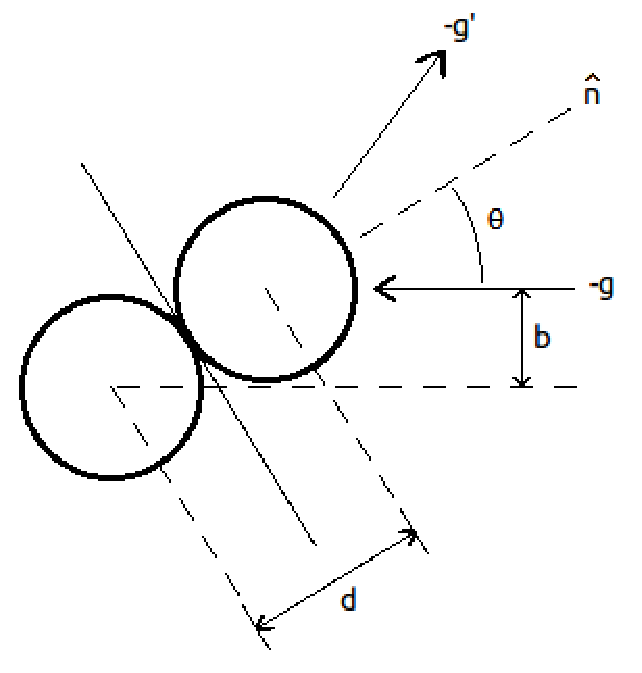
\includegraphics[angle=0,width=80mm]{Boltzmann/colliding_spheres.pdf}
\caption{Collision of two spheres}
\end{figure}
\FloatBarrier
% within the volume $g \, f \, dt \, dc_2 \, db \, d\epsilon$.
An illustration of the collision process can be seen in Figure~(\ref{colliding_spheres}). Consider the coordinate frame with the origin at the center of particle $p_2$ and the x-axis directed parallel to the vector of relative velocity $\vec{g}$. Let particle $p_1$ approach particle $p_2$ in this frame of reference with some offset $b$ at some azimuth angle $\epsilon$. During the time segment $dt$, particle $p_1$ will experience $f_2 g b \, dt \, d\vec{c}_2 \, db \, d\epsilon$ total collisions. We wish to sum over all possible values of the variables $b$, $\epsilon$ and $c$. These variables have constraints that must be determined for collision to happen. The offset $b$ must be between $0$ and the length of the particle diameter $b_*$ and $\epsilon$ can range from $0$ to $2 \pi$. Therefore, the total number of collisions per unit of time over some differential velocity segment $d\vec{c}$ is
%
\begin{equation}
\label{Collide}
\int_{\mathbb{R}^3} \int_0^{2 \pi} \int_0^{b_*} f f_1 g b \, db \, d\epsilon d\vec{c}_2 \, d\vec{c}.
\end{equation}
%
The term (\ref{Collide}) is known as the loss term and it accounts for particles with velocity $\vec{c}$ that will be lost in the result of colliding with other particles. At the same time, new particles with velocity $\vec{c}$ will be created as particles with velocities $\vec{c}'$ and $\vec{c}_1'$ collide at the offset $b$ and azimuth $\epsilon$. Let $f'=f(\vec{x},\vec{c}',t)$ and $f'_1=f(\vec{x},\vec{u}_1',t)$. The total number of particles with velocity $\vec{c}$ that are created during the collision process is given by the following integral known as the gain term
%
\begin{equation}
\label{invCollide}
\int_{\mathbb{R}^3} \int_0^{2 \pi} \int_0^{b_*} f' f_1' g b \, db \, d\epsilon d\vec{c}_1 \, d\vec{c}.
\end{equation}
%
Combining (\ref{Collide}) with (\ref{invCollide}) we arrive at the expression for the Boltzmann integral
%
\begin{equation*}
\label{BoltzmannRHS}
\Psi(f) = \int_{\mathbb{R}^3} \int_0^{2 \pi} \int_0^{b_*} \left( f' f_1' - f f_1 \right) g b \, db \, d\epsilon \, d\vec{c}_1.
\end{equation*}
%
Substituting this into (\ref{with_collision}) we obtain the Boltzmann equation
%
\begin{equation*}
\partial_t f + \vec{u} \cdot \nabla_x f = \int_{\mathbb{R}^3} \int_0^{2 \pi} \int_0^{b_*} \left( f' f_1' - f f_1 \right) \vec{g} b \, db \, d\epsilon \, d\vec{c}_1.
\end{equation*}
%
This is a non-linear integro-differential equation describing the evolution of $f(\vec{x},\vec{u},t)$.
%%%%%%%%%%%%%%%%%%%%%%%%%%%%%%%%%%%%%%%%%%%%%%%%%%%%%%%%%%%%%%%%%%%%%%%%%%%%
%%%%%%%%%%%%%%%%%%%%%%%%%%%%%%%%%%%%%%%%%%%%%%%%%%%%%%%%%%%%%%%%%%%%%%%%%%%%
%%%%%%%%%%%%%%%%%%%%%%%%%%%%%%%%%%%%%%%%%%%%%%%%%%%%%%%%%%%%%%%%%%%%%%%%%%%%
\subsection{The Maxwellian Distribution}
If the system of gas particles are not influenced by any outside intervention, then the distribution of gas particles will approach a state of equilibrium. The equilibrium distribution has the following form
%
\begin{equation}
\label{theDist}
f_0(\vec{u}; a,b,c) = a  \exp{\left(-\frac{||\vec{u} - \vec{c}||^2}{b^2}\right)}
\end{equation}
%
where constants $a$, $b$, and $\vec{c}$ depend on the state of gas and will be defined later. Traditionally, gas at the state of equilibrium is described using five parameters: gas density, temperature and the three components of the gas stream velocity. These parameters can be determined from the velocity distribution function by integration. Specifically, we have 
%
\begin{align*}
%\label{density}
n &= \int_{\mathbb{R}^3} f d\vec{u} \quad &\text{(Number Density)}\\
%\label{momentum}
\bar{u}_i &= \frac{1}{n} \int_{\mathbb{R}^3} u_i f d\vec{u} \quad &\text{(Average Velocity)}\\
&\text{and}\\
%\label{temperature}
T &= \frac{1}{3 n R} \int_{\mathbb{R}^3} ||u - \bar{u}||^2 f d\vec{u} \quad &\text{(Temperature)}.
\end{align*}
%
Where $R$ is the specific gas constant. As a consequence the Maxwellian equilibrium distribution takes the form
%
\begin{equation*}
%\label{Maxwellian}
f_M(\vec{u};n,\vec{\bar{u}},T,R) = \frac{n}{\sqrt{(2 \pi R T)^3}}  \exp{\left(-\frac{||\vec{u} - \vec{\bar{u}}||^2}{2 R T}\right)}
\end{equation*}
%
\begin{figure}[h!]
  \centering
      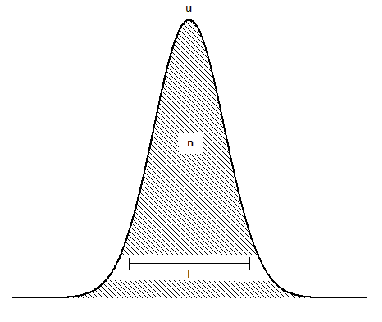
\includegraphics[angle=0,width=70mm]{Boltzmann/Maxwellian.pdf}
  \caption{\label{Max_fig}A Maxwellian distribution defined by the number density, bulk velocity and temperature.}
\end{figure}
\FloatBarrier
%
Figure~(\ref{Max_fig}) illustrates Maxwellian equilibrium distribution. The temperature is a quantity that describes how quickly the gas molecules are moving with respect to each other. The faster the molecules move, the higher the temperature and so the deviation from the mean velocity will be higher. The mean velocity we obtain from the average of the distribution function. The number density is the molecular count of the number of molecules in the gas and this is the area under the curve of the Maxwellian. When the gas has the distribution of the Maxwellian, we say the gas has reached a state of continuum.
%%%%%%%%%%%%%%%%%%%%%%%%%%%%%%%%%%%%%%%%%%%%%%%%%%%%%%%%%%%%%%%%%%%%%%%%%%%%
%%%%%%%%%%%%%%%%%%%%%%%%%%%%%%%%%%%%%%%%%%%%%%%%%%%%%%%%%%%%%%%%%%%%%%%%%%%%
%%%%%%%%%%%%%%%%%%%%%%%%%%%%%%%%%%%%%%%%%%%%%%%%%%%%%%%%%%%%%%%%%%%%%%%%%%%%
%%%%%%%%%%%%%%%%%%%%%%%%%%%%%%%%%%%%%%%%%%%%%%%%%%%%%%%%%%%%%%%%%%%%%%%%%%%%
%%%%%%%%%%%%%%%%%%%%%%%%%%%%%%%%%%%%%%%%%%%%%%%%%%%%%%%%%%%%%%%%%%%%%%%%%%%%
%%%%%%%%%%%%%%%%%%%%%%%%%%%%%%%%%%%%%%%%%%%%%%%%%%%%%%%%%%%%%%%%%%%%%%%%%%%%
%%%%%%%%%%%%%%%%%%%%%%%%%%%%%%%%%%%%%%%%%%%%%%%%%%%%%%%%%%%%%%%%%%%%%%%%%%%%
\section{Model Kinetic Equations}
To evaluate the Boltzmann collision operator we need to calculate a five fold integral. Integral in three dimensions in velocity space and in two dimensions in the collision impact parameter space. Because of the complexity of the collision integral closed form solutions to the Boltzmann equation are extremely difficult to obtain. Such solutions are only known in a few special cases. In general, one can only hope to compute approximate solutions numerically. However, even a numerical solution of the Boltzmann equation is extremely challenging because its straightforward discretization requires $O(n^{11})$ operations. We will look into the deterministic numerical solution of the Boltzmann equation in a later chapter. In this chapter, we are interested in the solutions to simpler approximate models of the Boltzmann equation. These models are the model kinetic equations. In 1954 Bhatnagar, Gross and Krook have proposed the BGK method in their paper \cite{bgk} to approximate the Boltzmann equation by replacing the collision integral with a term that relaxes the solution to the local Maxwellian. The BGK model supports the right hydrodynamic limit but its solution does not does not satisfy the Navier-Stokes equations. The problem is that the BGK model incorrectly predicts the Prandtl number. In particular, the number is always $1$ in the BGK solutions while for monotonic gases like Argon is expected to be about $2/3$. Later Holway \cite{esbgk} has proposed the Ellipsoidal-Statistical BGK or ES-BGK method which, similar to the BGK method, replaces the Boltzmann collision operator with a relaxation equation. The difference is that the target equilibrium distribution function in the ES-BGK model is a Gaussian distribution. The ES-BGK model achieves the correct Prandtl number. Also, it gives closer approximations to the Boltzmann equation at higher densities.
%%%%%%%%%%%%%%%%%%%%%%%%%%%%%%%%%%%%%%%%%%%%%%%%%%%%%%%%%%%%%%%%%%%%%%%%%%%%
%%%%%%%%%%%%%%%%%%%%%%%%%%%%%%%%%%%%%%%%%%%%%%%%%%%%%%%%%%%%%%%%%%%%%%%%%%%%
%%%%%%%%%%%%%%%%%%%%%%%%%%%%%%%%%%%%%%%%%%%%%%%%%%%%%%%%%%%%%%%%%%%%%%%%%%%%
%%%%%%%%%%%%%%%%%%%%%%%%%%%%%%%%%%%%%%%%%%%%%%%%%%%%%%%%%%%%%%%%%%%%%%%%%%%%
\subsection{The BGK Model}
In this section we will derive the kinetic BGK model and show that it conserves mass, momentum and energy which are the first three moments of the distribution function through velocity. This property of the BGK system is due to the fact that it relaxes the solution to the local Maxwellian. From Strutchtrup \cite{struchtrup}, we begin by taking the post collision terms and assuming they are near the Maxwellian $f_1' \approx f_{M 1}'$ and $f' \approx f_M'$. As a result, $f_M' f_{M1}' = f_M f_{M1}$ so then the collision integral term of the Boltzmann equation simplifies into
\begin{equation*}
f_m \int_{\mathbb{R}^3} \int_0^{2 \pi} \int_0^{b_*} f_{M1} g b db \, d\epsilon \, du' - f \int_{\mathbb{R}^3} \int_0^{2 \pi} \int_0^{b_*} f_1 g b db \, d\epsilon \, du'
\end{equation*}
%
We can assume that
\begin{equation*}
\label{difficultnu}
\nu = \int_{\mathbb{R}^3} \int_0^{2 \pi} \int_0^{b_*} f_{M1} g b db \, d\epsilon \, du' \approx \int_{\mathbb{R}^3} \int_0^{2 \pi} \int_0^{b_*} f_1 g b db \, d\epsilon \, du'
\end{equation*}
%
Where we arrive at the BGK collision operator
\begin{equation}
\label{BGK}
\Psi_{BGK}(f) = \nu_{BGK} \left(f_M - f \right).
\end{equation}
%
The BGK equation takes the form
%
\begin{equation}
\label{BGKeq}
\partial_t f + \vec{u} \cdot \nabla_x f = \nu_{BGK} \left(f_M - f \right).
\end{equation}
%
Because it is impractical to compute the collision frequency using formula (\ref{difficultnu}), it usually replaced by the mean the mean collision frequency as a ratio of the pressure and the dynamic viscosity
\begin{equation}
\label{collision}
\nu_{BGK} = \frac{P}{\mu}.
\end{equation}
%
Where the dynamic viscosity is computed from
\begin{equation}
\mu = \mu_0 (T/T_{ref})^{\alpha_{gas}}
\end{equation}
%
and the pressure is obtained from $P = n k T$ where $n$ is the number density and $k$ is the Boltzmann constant. Let us compute the first three moments of ($\ref{BGK}$), obtained by a multiplication of the BGK operator $\Psi$ by the functions $\{ 1, u_i, ||\vec{u} - \vec{\bar{u}}||^2 \}$:
%
\begin{itemize}
%%%%%%%%%%%%%%%%%%%%%%%%%%%%%%%%%%%%%%%%%%%%%%%%%%%%%%%%%%%%%%%%%%%%%%%%%%%%%%%%%%%%
\item Case \{ $1$ \}
%
\begin{align*}
\int_{\mathbb{R}^3} \Psi_{BGK} (f) d\vec{u} &= \int_{\mathbb{R}^3} \nu (f_M - f) d\vec{u}\\
&= \nu \left(\int_{\mathbb{R}^3} \frac{n}{\sqrt{(2 \pi R T)^3}} e^{-\frac{||\vec{u} - \vec{\bar{u}}||^2}{2 R T}} d\vec{u} - \int_{\mathbb{R}^3} f d\vec{u} \right)\nonumber \\
&= \nu \left( \frac{n}{\sqrt{(2 \pi R T)^3}} \int_{\mathbb{R}^3} e^{-\frac{||\vec{u} - \vec{\bar{u}}||^2}{2 R T}} d\vec{u} - n \right)\nonumber \\
&= \nu (n - n) = 0.
\end{align*}
%%%%%%%%%%%%%%%%%%%%%%%%%%%%%%%%%%%%%%%%%%%%%%%%%%%%%%%%%%%%%%%%%%%%%%%%%%%%%%%%%%%%
\item Case \{ $u_i$ \}
%
\begin{align*}
\int_{\mathbb{R}^3} &u_i \Psi_{BGK} (f) d\vec{u} = \nu \int_{\mathbb{R}^3} u_i (f_M - f) d\vec{u} \nonumber \\
&= \nu \left( \frac{n}{\sqrt{(2 \pi R T)^3}} \int_{\mathbb{R}^3} u_i e^{-\frac{||\vec{u} - \vec{\bar{u}}||^2}{2 R T}} d\vec{u} - \int_{\mathbb{R}} u_i f d\vec{u} \right)\nonumber \\
&= \nu \left( \frac{n}{\sqrt{(2 \pi R T)^3}} \int_{\mathbb{R}^3} u_i e^{-\frac{(u_i - \bar{u}_i)^2}{2 R T}} du_i \prod_{j=1,3 \atop j \ne i} \int_{\mathbb{R}^3} e^{-\frac{(u_j - \bar{u}_j)^2}{2 R T}} du_j - n \bar{u}_j \right) \nonumber
\end{align*}
%
we can shift the domain by $(\bar{u}_1,\bar{u}_2,\bar{u}_3)$ so that the exponential is centered at zero and set $v_k = u_k/(2 R T)$ for $k=1,2,3$ to get
%
\begin{align*}
= \nu \left( \frac{n \sqrt{(2 R T)^3}}{\sqrt{(2 \pi R T)^3}} \int_{\mathbb{R}^3} (\sqrt{2 R T} v_i + \bar{u}_i) e^{-v_i^2} dv_i \prod_{j=1,3 \atop j \ne i} \int_{\mathbb{R}^3} e^{-v_j^2} dv_j - n \bar{u}_j \right).
\end{align*}
%
Notice that $\int v_i  \exp{\left(-v_i^2\right)} d v_i$ is finite over any domain and odd about zero and so its evaluation over $\mathbb{R}$ is zero. Recalling that $\int_{\mathbb{R}}  \exp{\left(-v_j^2\right)} dv_j = \sqrt{\pi}$ we obtain
%
\begin{equation*}
= \nu (n u_i - n u_i) = 0.
\end{equation*}
%%%%%%%%%%%%%%%%%%%%%%%%%%%%%%%%%%%%%%%%%%%%%%%%%%%%%%%%%%%%%%%%%%%%%%%%%%%%%%%%%%%%
\item Case \{ $||\vec{u} - \vec{\bar{u}}||^2$ \}
%
\begin{align*}
&\int_{\mathbb{R}^3} ||\vec{u} - \vec{\bar{u}}||^2 \Psi_{BGK} (f) d\vec{u} = \nu \int_{\mathbb{R}^3} ||\vec{u} - \vec{\bar{u}}||^2 (f_M - f) d\vec{u}\\
&= \nu \left( \frac{n}{\sqrt{(2 \pi R T)^3}} \int_{\mathbb{R}^3} ||\vec{u} - \vec{\bar{u}}||^2 e^{-\frac{||\vec{u} - \vec{\bar{u}}||^2}{2 R T}} d\vec{u} - \int_{\mathbb{R}} ||\vec{u} - \vec{\bar{u}}||^2 f d\vec{u} \right)\nonumber \\
&= \nu \left( \frac{n}{\sqrt{(2 \pi R T)^3}} \sum_{i=1,2,3} \int_{\mathbb{R}^3} (u_i - \bar{u}_i)^2 e^{-\frac{||u_i - \bar{u}_i||^2}{2 R T}} du_i - 3 n R T \right)\nonumber \\
&= \nu \frac{n}{\sqrt{(2 \pi R T)^3}} \sum_{i=1,2,3} \int_{\mathbb{R}} (u_i - \bar{u}_i)^2 e^{-\frac{(u_i - \bar{u}_i)^2}{2 R T}} du_i \prod_{j=1,2,3 \atop j \ne i} \int_{\mathbb{R}} e^{-\frac{(u_j - \bar{u}_j)^2}{2 R T}} du_j\\
& \, - \nu 3 n R T
\end{align*}
%
We shift by $(u_1,u_2,u_3)$ to get
%
\begin{align*}
= \nu \left( \frac{n}{\sqrt{(2 \pi R T)^3}} \sum_{i=1,2,3} \int_{\mathbb{R}} u_i^2 e^{-\frac{u_i^2}{2 R T}} du_i \prod_{j=1,2,3 \atop j \ne i} \int_{\mathbb{R}} e^{-\frac{u_i^2}{2 R T}} du_j  - 3 n R T \right)
\end{align*}
%
By a change of variables by letting $\sqrt{2 R T} v_i = u_i$, we have
%
\begin{align*}
&= \nu \frac{n}{\sqrt{(2 \pi R T)^3}} \sum_{i=1,2,3} 2 R T \sqrt{(2 R T)^3} \int_{\mathbb{R}^3} v_i^2 e^{-v_i^2} dv_i \prod_{j=1,2,3 \atop j \ne i} \int_{\mathbb{R}} e^{-v_i^2} dv_j\\
& \, - \nu 3 n R T\\
&= \nu \left( \frac{2 n R T \pi}{\sqrt{\pi^3}} \sum_{i=1,2,3} \int_{\mathbb{R}^3} v_i^2 e^{-v_i^2} dv_i - 3 n R T \right)\\
\end{align*}
%
We then proceed to integrate by parts by separating the integral components into $v_i$ and $v_i e^{-v_i^2} dv_i$ which yields
%
\begin{align}
&= \nu \left( \frac{2 n R T \pi}{\sqrt{\pi^3}} \sum_{i=1,2,3} \left(-\frac{1}{2} v_i e^{-v_i^2}|_{-\infty}^\infty + \frac{1}{2} \int_{\mathbb{R}} e^{-v_i^2} dv_i \right) - 3 n R T \right)\nonumber \\
&= \nu \left(3 n R T - 3 n R T \right) = 0.
\end{align}
\end{itemize}
%
And so we conclude the first five moments of the BGK equation are conserved:
%
\begin{align*}
\int_{\mathbb{R}^3} \Psi_{BGK} (f) d\vec{u} &= 0 \quad & (\text{Mass})\\
\int_{\mathbb{R}^3} \left( \begin{array}{c} u_1 \\ u_2 \\ u_3 \end{array} \right) \Psi_{BGK} (f) d\vec{u} &= \left( \begin{array}{c} 0 \\ 0 \\ 0 \end{array} \right) \quad & (\text{Momentum}) \\
\text{and}\\
\int_{\mathbb{R}^3} ||\vec{u} - \vec{\bar{u}}||^2 \Psi_{BGK} (f) d\vec{u} &= 0 \quad & (\text{Temperature})\\
\end{align*}
%
%%%%%%%%%%%%%%%%%%%%%%%%%%%%%%%%%%%%%%%%%%%%%%%%%%%%%%%%%%%%%%%%%%%%%%%%%%%%
%%%%%%%%%%%%%%%%%%%%%%%%%%%%%%%%%%%%%%%%%%%%%%%%%%%%%%%%%%%%%%%%%%%%%%%%%%%%
%%%%%%%%%%%%%%%%%%%%%%%%%%%%%%%%%%%%%%%%%%%%%%%%%%%%%%%%%%%%%%%%%%%%%%%%%%%%
%%%%%%%%%%%%%%%%%%%%%%%%%%%%%%%%%%%%%%%%%%%%%%%%%%%%%%%%%%%%%%%%%%%%%%%%%%%%
%%%%%%%%%%%%%%%%%%%%%%%%%%%%%%%%%%%%%%%%%%%%%%%%%%%%%%%%%%%%%%%%%%%%%%%%%%%%
%%%%%%%%%%%%%%%%%%%%%%%%%%%%%%%%%%%%%%%%%%%%%%%%%%%%%%%%%%%%%%%%%%%%%%%%%%%%
%%%%%%%%%%%%%%%%%%%%%%%%%%%%%%%%%%%%%%%%%%%%%%%%%%%%%%%%%%%%%%%%%%%%%%%%%%%%
\subsection{The ES-BGK Model}
Holway [10] proposed a modification to the BGK model, known as the ellipsoidal-statistical BGK model that achieves the correct Prandtl number. According to Andries \cite{andries} the BGK model has been shown to produce satisfactory results and, a first order Chapman-Enskog expansion applied to ($\ref{BGK}$) gives the correct Navier-Stokes viscosity $\mu$ but gives a heat conduction of $\kappa = (5/2)R \mu$ which results in a Prandtl number of
\begin{equation}
\label{Prandtl}
Pr = \frac{5 R \mu }{2 \kappa} = 1.
\end{equation}
%
For monotonic gases like Argon, the desired Prandtl number is near $Pr = 2/3$ and so the BGK approximation will fail to give the correct Navier-Stokes heat conduction. The ES-BGK model corrects the Prandtl number by the use of an adjustment factor $\alpha$:
%
\begin{equation}
Pr = \frac{1}{1 - \alpha}
\end{equation}
%
where $\alpha$ is a parameter in the tensor 
%
\begin{equation}
\mathbb{T} = (1-\alpha)RT I + \alpha \Theta
\end{equation}
%
and
%
\begin{equation}
\label{Theta}
\Theta_{ij} := \frac{1}{n} \int_{\mathbb{R}^{3}} c_i c_j f \, d\vec{u}.
\end{equation}
%
The ES-BGK relaxation term is
%L.H. Holway. Kinetic theory of shock structure using an ellipsoidal distribution function, in: Rarefied Gas Dynamics, vol. I (Proceedings of the Fourth International Symposium, University of Toronto, 1964), Academic Press, New York, 1966, pp. 193–215.%
%
\begin{equation}
\label{Gaussian}
f_{ES} = \frac{n}{\sqrt{\det(2 \pi \bar{\bar{\mathbb{T}}})}}  \exp{\left(-\frac{\vec{c}' \bar{\bar{\mathbb{T}}}^{-1} \vec{c}}{2}\right)}
\end{equation}
%
where $\vec{c} = \vec{u} - \bar{\vec{u}}$ is the pecular velocity. $f_{ES}$ replaces the Maxwellian in (\ref{BGK}). We expect (\ref{Gaussian}) to approach zero for large values of $\vec{u}$. Also form physical considerations we need $\alpha$ to be chosen so that $\mathbb{T}^{-1}$ or $\mathbb{T}$ is positive definite. Zheng \cite{zheng} has shown that if we restrict $\alpha \in [-\frac{1}{2},1)$, then we preserve the positive definite behavior of $\mathbb{T}$.

The collision frequency for the ES-BGK model is
%
\begin{equation}
\nu_{ES} = \frac{P}{(1 - \alpha) \mu}
\end{equation}
%
and the ES-BGK collision operator takes the form of
%
\begin{equation}
\label{ESBGK}
\Psi_{ES}(f) = \nu_{ES} \left(f_{ES} - f \right)
\end{equation}
%
giving us the ES-BGK equation
%
\begin{equation}
\label{ESBGKeq}
\partial_t f + \vec{u} \cdot \nabla_x f = \nu_{ES} \left(f_{ES} - f \right).
\end{equation}
%
Notice that when $\alpha = 0$ we obtain the original BGK model back suggesting that the ES-BGK model generalizes the BGK model.
%Maximum entropy derivation Junk, M.: Maximum entropy for reduced moment problems. M3AS 10, 1121–1149 (2000)
%%%%%%%%%%%%%%%%%%%%%%%%%%%%%%%%%%%%%%%%%%%%%%%%%%%%%%%%%%%%%%%%%%%%%%%%%%%%%%%%%%%%%%%%%%%
%%%%%%%%%%%%%%%%%%%%%%%%%%%%%%%%%%%%%%%%%%%%%%%%%%%%%%%%%%%%%%%%%%%%%%%%%%%%%%%%%%%%%%%%%%%
%%%%%%%%%%%%%%%%%%%%%%%%%%%%%%%%%%%%%%%%%%%%%%%%%%%%%%%%%%%%%%%%%%%%%%%%%%%%%%%%%%%%%%%%%%%
%%%%%%%%%%%%%%%%%%%%%%%%%%%%%%%%%%%%%%%%%%%%%%%%%%%%%%%%%%%%%%%%%%%%%%%%%%%%%%%%%%%%%%%%%%%
\section{One Dimensional Reduction}
It is in our interest in the rest of this chapter to compute the solution to the model equations constrained to one dimension. We can assume that the solution is not changing in two of the three spatial dimensions that we will denoted as $y$ and $z$. In a physical sense, the gas is held between two infinitely long parallel plates where the mass flux along the planar directions is zero. Reducing our problem to one dimension and using the approximate kinetic models will reduce the computational effort because the integration is done in only one dimension. With this assumption, our objective here is to reduce the three dimensional kinetic model to two separate hyperbolic PDEs of similar form that will be tied together by the calculation of the macro parameters. To accomplish this, we start with introducing the reduced distribution functions $h(x,u_1,t)$ and $g(x,u_1,t)$ by integrating the distribution function $f(\vec{x},\vec{u},t)$ through velocity in the $u_2$ and $u_3$ directions and integrating the product of $f$ and the velocity $u_2$ (in $y$ direction) through $u_2$ and $u_3$ directions of velocity
%
\begin{equation}
\label{f1}
h(x,u_1,t) = \int_{\mathbb{R}^2} f du_2 du_3
\end{equation}
%
and
%
\begin{equation}
\label{f2}
g(x,u_1,t) = \int_{\mathbb{R}^2} u_2^2 f du_2 du_3
\end{equation}
%
which, as we will soon see, will be the catalyst in the reduction process.
%%%%%%%%%%%%%%%%%%%%%%%%%%%%%%%%%%%%%%%%%%%%%%%%%%%%%%%%%%%%%%%%%%%%%%%%%%%%%%%%%%%%%%%%%%%%%%%%%%%%%%%%%%%%%%%%%%%%%%%%%
\subsection{Reduction of the Macro Parameters}
In this section, we will reduce the macro parameters to one dimension. The density can be written as
%
\begin{align*}
n &= \int_{\mathbb{R}^3} f d\vec{u}\\
&= \int_{\mathbb{R}} \left( \int_{\mathbb{R}^2} f du_2 du_3 \right) du_1\\
&= \int_{\mathbb{R}} h du_1.
\end{align*}
%
Next we will reduce the bulk velocity. For the $i^{th}$ component of the bulk velocity we obtain
%
\begin{align*}
\bar{u}_i &= \frac{1}{n} \int_{\mathbb{R}^3} u_i f d\vec{u}\\
&= \frac{1}{n} \int_{\mathbb{R}} \left( \int_{\mathbb{R}^2} u_i f du_2 du_3 \right) du_1
\end{align*}
%
but because there is no mass exchange expected in the $y$ and $z$ directions we obtain
%
\begin{equation*}
\bar{u}_i = \frac{1}{n} \left \{ \begin{array}{cc} \int_{\mathbb{R}} u_1 h du_1 & i=1\\ 0 & i = 2,3 \end{array} \right. .
\end{equation*}
%
The temperature
%
\begin{align*}
T &= \frac{1}{3 n R} \int_{\mathbb{R}^3} ||u - \bar{u}||^2 f d\vec{u}\\
&= \frac{1}{3 n R} \int_{\mathbb{R}^3} \left( ||\vec{u}||^2 - 2 \vec{u} \cdot \vec{\bar{u}} + ||\vec{\bar{u}}||^2 \right) f d\vec{u}\\
\end{align*}
%
because the bulk velocity is only in the $x$ direction, we have that $\bar{u}_2 = 0 = \bar{u}_3$ and so
%
\begin{align*}
&= \frac{1}{3 n R} \int_{\mathbb{R}^3} \left( (u_1^2 + u_2^2 + u_3^2) - 2 u_1 \bar{u}_1 + \bar{u}_1^2 \right) f d\vec{u}\\
&= \frac{1}{3 n R} \int_{\mathbb{R}^3} \left( (u_1 - \bar{u_1})^2 + (u_2^2 + u_3^2)\right) f d\vec{u}\\
&= \frac{1}{3 n R} \int_{\mathbb{R}} \left( (u_1 - \bar{u_1})^2 \right) f du_1\\
& \, + \frac{1}{3 n R} \int_{\mathbb{R}^2} \left( (u_2^2 + u_3^2)\right) f du_2 du_3
\end{align*}
%
based on our symmetry assumption that nothing changes in the $y$ and $z$ directions
%
\begin{equation*}
\int_{\mathbb{R}^3} u_2^2 f du_2 du_3 = \int_{\mathbb{R}^3} u_3^2 f du_2 du_3
\end{equation*}
%
we obtain
%
\begin{equation*}
T = \frac{1}{3 n R} \int_{\mathbb{R}} \left( (u - \bar{u})^2 h + 2 g \right) du_1.
\end{equation*}
%%%%%%%%%%%%%%%%%%%%%%%%%%%%%%%%%%%%%%%%%%%%%%%%%%%%%%%%%%%%%%%%%%%%%%%%%%%%%%%%%%%%%%%%%%%%%%%
%%%%%%%%%%%%%%%%%%%%%%%%%%%%%%%%%%%%%%%%%%%%%%%%%%%%%%%%%%%%%%%%%%%%%%%%%%%%%%%%%%%%%%%%%%%%%%%
%%%%%%%%%%%%%%%%%%%%%%%%%%%%%%%%%%%%%%%%%%%%%%%%%%%%%%%%%%%%%%%%%%%%%%%%%%%%%%%%%%%%%%%%%%%%%%%
%%%%%%%%%%%%%%%%%%%%%%%%%%%%%%%%%%%%%%%%%%%%%%%%%%%%%%%%%%%%%%%%%%%%%%%%%%%%%%%%%%%%%%%%%%%%%%%
\subsection{Reduction of the Kinetic Model}
We begin now to reduce the equation
%
\begin{equation}
\label{kineticModel}
\partial_t f + \vec{u} \cdot \nabla_x f = \nu \left( f_0 - f \right).
\end{equation}
%
to one dimension. Since it is our assumption that the gas is homogeneous in the $y$ and $z$ directions, there is no change and so we expect $\vec{u} \cdot \nabla_x = u \partial_x$. As a result (\ref{kineticModel}) reduces to
%
\begin{equation}
\label{reduction1}
\partial_t f + u \partial_x f = \nu \left( f_0 - f \right).
\end{equation}
%
Now $f$ is still a function of $\vec{x}$ and $\vec{u}$. To reduce the equation to one dimension. The first step is to integrate (\ref{reduction1}) in the $u_2$ and $u_3$ directions and to obtain an equation with $h$. In the second step we multiply (\ref{reduction1}) by $u_2^2$ then integrate in the $u_2$ and $u_3$ directions to get an evolution equation with $g$.
%
\begin{equation}
\label{eq659}
\int_{\mathbb{R}^2} \partial_t f du_2 du_3 + \int_{\mathbb{R}^2} u_1 \partial_x f du_2 du_3 = \int_{\mathbb{R}^2} \nu \left( f_0 - f \right) du_2 du_3
\end{equation}
%
We can immediately see that by substituting (\ref{f1}) into (\ref{eq659}) the equation reduces to
%
\begin{equation*}
\partial_t h + u_1 \, \partial_x h = \int_{\mathbb{R}^2} \nu \left( f_0 - f \right) du_2 du_3.
\end{equation*}
%
Moreover, because of the linearity of the integral we obtain the following form for the right hand side of the equation
%
\begin{equation}
\label{f1Part}
\int_{\mathbb{R}^2} \nu \left( f_0 - f \right) \, du_2 \, du_3 = \nu \left( \int_{\mathbb{R}^2} f_0 \, du_2 \, du_3 - h \right).
\end{equation}
%
To complete the second step we multiply (\ref{reduction1}) by $u_2^2$
%
\begin{equation*}
u_2^2 \, \partial_t f + u_2^2 \, u_1 \, \partial_x f = u_2^2 \, \nu \, \left( f_0 - f \right).
\end{equation*}
%
and integrate through $u_2$ and $u_3$.
%
\begin{equation*}
\int_{\mathbb{R}^2} u_2^2 \partial_t f du_2 du_3 + \int_{\mathbb{R}^2} u_2^2 u_1 \partial_x f du_2 du_3 = \int_{\mathbb{R}^2} u_2^2 \nu \left( f_0 - f \right) du_2 du_3
\end{equation*}
%
\begin{equation*}
\partial_t \int_{\mathbb{R}^2} u_2^2 f du_2 du_3 + u_1 \partial_x \int_{\mathbb{R}^2} u_2^2 f du_2 du_3 = \nu \left( \int_{\mathbb{R}^2} u_2^2 f_0 du_2 du_3 - \int_{\mathbb{R}^2} u_2^2 f du_2 du_3 \right)
\end{equation*}
%
\begin{equation}
\label{f2Party}
\partial_t g + u_1 \partial_x g = \nu \left( \int_{\mathbb{R}^2} u_2^2 f_0 du_2 du_3 - g \right)
\end{equation}
%
which is our second equation. From here, all that is left is to state the formulas for evaluating the equilibrium distributions in BGK and ES-BGK models in terms of $h$ and $g$. Since $f_0$ is a function of $\vec{u}$, careful consideration is required. This step will depend on the kinetic model we are using therefore we consider the integrals for the BGK and ESBGK models separately below.
%%%%%%%%%%%%%%%%%%%%%%%%%%%%%%%%%%%%%%%%%%%%%%%%%%%%%%%%%%%%%%%%%%%%%%%%%%%%%%%%%%%%%%%%%%%%
%%%%%%%%%%%%%%%%%%%%%%%%%%%%%%%%%%%%%%%%%%%%%%%%%%%%%%%%%%%%%%%%%%%%%%%%%%%%%%%%%%%%%%%%%%%%
%%%%%%%%%%%%%%%%%%%%%%%%%%%%%%%%%%%%%%%%%%%%%%%%%%%%%%%%%%%%%%%%%%%%%%%%%%%%%%%%%%%%%%%%%%%%
%%%%%%%%%%%%%%%%%%%%%%%%%%%%%%%%%%%%%%%%%%%%%%%%%%%%%%%%%%%%%%%%%%%%%%%%%%%%%%%%%%%%%%%%%%%%
%%%%%%%%%%%%%%%%%%%%%%%%%%%%%%%%%%%%%%%%%%%%%%%%%%%%%%%%%%%%%%%%%%%%%%%%%%%%%%%%%%%%%%%%%%%%
\subsection{Reduction of the Maxwellian Distribution}
In the BGK model, we have a Maxwellian distribution $f_0 = f_{BGK} = f_M$ and so we can explicitly evaluate the integral of the Maxwellian through $u_2$ and $u_3$
%
\begin{align}
\label{480}
\int_{\mathbb{R}^2} f_0 du_2 du_3 &= \int_{\mathbb{R}^2} \frac{n}{\sqrt{(2 \pi RT)^3}}  \exp{\left(-\frac{||\vec{u} - \vec{\bar{u}}||^2}{2 RT}\right)} du_2 du_3\\
\end{align}
%
and $\vec{\bar{u}} = (\bar{u}_1,0,0)$ then
%
\begin{align*}
&= \frac{n}{\sqrt{(2 \pi RT)^3}} \int_{\mathbb{R}^2}  \exp{\left(-\frac{||u_1 - \bar{u}_1||^2 + u_2^2 + u_3^2}{2 RT}\right)} du_2 du_3\\
&= \frac{n}{\sqrt{(2 \pi RT)^3}}  \exp{\left(-\frac{(u - \bar{u})^2}{2 RT}\right)} \int_{\mathbb{R}^2}  \exp{\left(-\frac{(u_2^2 + u_3^2)}{2 RT}\right)} du_2 du_3.\\
\end{align*}
%
Let $r^2 = u_2^2 + u_3^2$, $r \cos(\theta) = u_2$ and $r \sin(\theta) = u_3$ then
%
\begin{align*}
\int_{\mathbb{R}^2}  \exp{\left(-\frac{(u_2^2 + u_3^2)}{2 RT}\right)} du_2 du_3 &= \int_0^\infty \int_0^{2 \pi}  \exp{\left(-\frac{(r^2)}{2 RT}\right)} r d\theta dr\\
&= 2 \pi RT.
\end{align*}
%
then (\ref{480}) becomes
%
\begin{equation*}
\int_{\mathbb{R}^2} f_0 du_2 du_3 = \frac{n}{\sqrt{2 \pi RT}}  \exp{\left(-\frac{(u - \bar{u})^2}{2 RT}\right)}.
\end{equation*}
%
Now through a similar process, we will evaluate the product of the distribution function with $u_2^2$.
%
\begin{align*}
\int_{\mathbb{R}^2}& u_2^2 f_0 du_2 du_3 = \int_{\mathbb{R}^2} u_2^2 \frac{n}{\sqrt{(2 \pi RT)^3}}  \exp{\left(-\frac{(u - \bar{u})^2}{2 RT}\right)} du_2 du_3\\
&= \frac{n}{\sqrt{(2 \pi RT)^3}} \int_{\mathbb{R}^2} u_2^2  \exp{\left(-\frac{(u - \bar{u})^2}{2 RT} \right)} du_2 du_3\\
&= \frac{n}{\sqrt{(2 \pi RT)^3}}  \exp{\left(-\frac{(u - \bar{u})^2}{2 RT}\right)} \int_{\mathbb{R}^2} u_2^2  \exp{\left(-\frac{(v^2 + w^2)}{2 RT}\right)} du_2 du_3\\
&= \frac{n}{\sqrt{(2 \pi RT)^3}}  \exp{\left(-\frac{(u - \bar{u})^2}{2 RT}\right)} \int_{\mathbb{R}} u_2^2  \exp{\left(-\frac{u_2^2}{2 RT}\right)} du_2 \int_{\mathbb{R}}  \exp{\left(-\frac{u_3^2}{2 RT}\right)} du_3\\
\end{align*}
%
By adjusting the integral
%
\begin{equation}
\int_{\mathbb{R}} u_2^2  \exp{\left(-\frac{u_2^2}{2 RT}\right)} du_2 = (2 R T)^{3/2} \int_{\mathbb{R}} u_2^2  \exp{\left(-u_2^2\right)} du_2
\end{equation}
%
and evaluating by parts by letting $v = u_2$ and $d w = u_2  \exp{\left(-u_2^2\right)} \, du_2$ we obtain
%
\begin{equation}
= 2 (2 R T)^{3/2} \left(-\frac{1}{2} u_2  \exp{\left(-u_2^2\right)}|_{-\infty}^\infty + \frac{1}{2} \int_{\mathbb{R}}  \exp{\left(-u_2^2\right)} \, du_2 \right) = (R T)^{3/2} \sqrt{2 \pi}.
\end{equation}
%
Then we obtain
%
\begin{align*}
\int_{\mathbb{R}^2} u_2^2 f_0 du_2 du_3 &= \frac{n}{\sqrt{(2 \pi RT)^3}}  \exp{\left(-\frac{(u - \bar{u})^2}{2 RT}\right)} \left((R T)^{3/2} \sqrt{2 \pi} \right) \left( \sqrt{2 \pi R T} \right) \\
&= n \sqrt{\frac{R T}{2 \pi}}  \exp{\left(-\frac{(u - \bar{u})^2}{2 RT}\right)}
\end{align*}
%
which is the reduced Maxwellian distribution function in one dimension. The BGK equations in one dimension take the form:
%
\begin{equation*}
\partial_t h + u_1 \partial_x h = \nu_{BGK} \left(\frac{n}{\sqrt{2 \pi RT}}  \exp{\left(-\frac{(u_1 - \bar{u}_1)^2}{2 RT}\right)} - h \right)
\end{equation*}
%
\begin{equation*}
\partial_t g + u_1 \partial_x g = \nu_{BGK} \left( n \sqrt{\frac{R T}{2 \pi}}  \exp{\left(-\frac{(u - \bar{u})^2}{2 RT}\right)} - g \right)
\end{equation*}
%%%%%%%%%%%%%%%%%%%%%%%%%%%%%%%%%%%%%%%%%%%%%%%%%%%%%%%%%%%%%%%%%%%%%%%%%%%%%%%%%%%%%%%%%%%%
%%%%%%%%%%%%%%%%%%%%%%%%%%%%%%%%%%%%%%%%%%%%%%%%%%%%%%%%%%%%%%%%%%%%%%%%%%%%%%%%%%%%%%%%%%%%
%%%%%%%%%%%%%%%%%%%%%%%%%%%%%%%%%%%%%%%%%%%%%%%%%%%%%%%%%%%%%%%%%%%%%%%%%%%%%%%%%%%%%%%%%%%%
%%%%%%%%%%%%%%%%%%%%%%%%%%%%%%%%%%%%%%%%%%%%%%%%%%%%%%%%%%%%%%%%%%%%%%%%%%%%%%%%%%%%%%%%%%%%
%%%%%%%%%%%%%%%%%%%%%%%%%%%%%%%%%%%%%%%%%%%%%%%%%%%%%%%%%%%%%%%%%%%%%%%%%%%%%%%%%%%%%%%%%%%%
\subsection{Reduction of the Gaussian Distribution Function for ES-BGK}
For the ES-BGK model, recall that the Maxwellian distribution is replaced with a general Gaussian distribution:
%
\begin{equation}
\label{fES}
f_0 = f_{ES} = \frac{n}{\sqrt{\det{\left(2 \pi \mathbb{T}\right)}}} \ \exp{\left(-\frac{c' \mathbb{T}^{-1} c}{2} \right)}
\end{equation}
%
as defined by (\ref{Gaussian}) where $\mathbb{T} = (1 - \alpha) RT \mathbb{I} + \alpha \Theta$ and
%
\begin{equation}
\label{Theta_component}
\Theta_{ij} := \frac{1}{n} \int_{\mathbb{R}^{3}} c_i c_j f du
\end{equation}
%
is from (\ref{Theta}). Expanding $\Theta_{i,j}$:
%
\begin{align*}
\Theta_{i,j} &= \frac{1}{n} \int_{\mathbb{R}} c_i c_j f d\vec{u} = \frac{1}{n} \int_{\mathbb{R}} (u_i - \bar{u}_i)(u_j - \bar{u}_j) f d\vec{u}\\
&= \frac{1}{n} \int_{\mathbb{R}} \left( u_i u_j f - u_i \bar{u}_j f - \bar{u}_i u_j f + \bar{u}_i \bar{u}_j f \right) d\vec{u}.
\end{align*}
%
From our assumption that the bulk of the velocity only changes in the $x$ direction we obtain
%
\begin{equation*}
\int_{\mathbb{R}} u_i f d\vec{u} = \bar{u}_i = \left \{ \begin{array}{cc} 0, & i \neq 1\\ \bar{u}_1, & i = 1 \end{array} \right.
\end{equation*}
%
so then the off diagonal components of (\ref{Theta_component}) are zero and for the diagonal components we obtain
%
\begin{equation*}
\Theta_{i,i} = \left \{ \begin{array}{cc} \int_{\mathbb{R}} (u_1 - \bar{u}_1)^2 f_1 du_1, & i = 1\\ \int_{\mathbb{R}} f_2 du_1, & i = 2,3 \end{array} \right..
\end{equation*}
%
One can see that we have $tr(\Theta) = 3 n R T$. Because the off diagonals are zero, $\det(2 \pi \mathbb{T}) = (2 \pi)^3 \prod_{i=1}^3 
\mathbb{T}_{i,i}$ and 
%
\begin{equation*}
\mathbb{T}_{i,j}^{-1} = \left \{ \begin{array}{cc} \frac{1}{\mathbb{T}_{i,i}}, & i=j\\ 0, & i \neq j \end{array} \right. .
\end{equation*}
%
In the numerator of the exponent of (\ref{fES}) we obtain
%
\begin{equation*}
c' \mathbb{T}^{-1} c = (u_1 - \bar{u}_1)^2 \mathbb{T}_1^{-1} + (u_2^2 + u_3^2) \mathbb{T}_2^{-1}.
\end{equation*}
%
Finally (\ref{fES}) becomes
%
\begin{equation}
\label{1D_ES}
f_{ES} = \frac{n}{\sqrt{(2 \pi)^3 \mathbb{T}_1 \mathbb{T}_2^2}} \ \exp{\left(-\frac{1}{2} \left( (u_1 - \bar{u}_1)^2 \mathbb{T}_1^{-1} + (u_2^2 + u_3^2) \mathbb{T}_2^{-1} \right) \right)}.
\end{equation}
%
Evaluating the integral of (\ref{1D_ES}) through $u_2$ and $u_3$
%
\begin{align*}
&\int_{\mathbb{R}^2} f_{ES} d u_2 d u_3 =\\
&= \int_{\mathbb{R}^2} \frac{n}{\sqrt{(2 \pi)^3 \mathbb{T}_1 \mathbb{T}_2^2}} \ \exp{\left(-\frac{1}{2} \left( (u_1 - \bar{u}_1)^2 \mathbb{T}_1^{-1} + (u_2^2 + u_3^2) \mathbb{T}_2^{-1} \right) \right)} du_2 du_3\\
&= \frac{n}{\sqrt{(2 \pi)^3 \mathbb{T}_1 \mathbb{T}_2^2}} \ \exp{\left(-\frac{1}{2} \left( (u_1 - \bar{u}_1)^2 \mathbb{T}_1^{-1} \right) \right)} \int_{\mathbb{R}^2} \ \exp{\left(-\frac{1}{2} \left( (u_2^2 + u_3^2) \mathbb{T}_2^{-1} \right) \right)} du_2 du_3\\
&= \frac{n}{\sqrt{2 \pi \mathbb{T}_1}} \ \exp{\left(-\frac{1}{2} \left( (u_1 - \bar{u}_1)^2 \mathbb{T}_1^{-1} \right) \right)}.
\end{align*}
%
To obtain the second evolution equation, we will need to also consider the integral of the product of $u_2^2$ and (\ref{1D_ES}) through all of $u_2$ and $u_3$
%
\begin{align*}
&\int_{\mathbb{R}^2} u_2^2 f_{ES} d u_2 d u_3 =\\
&= \frac{n}{\sqrt{(2 \pi)^3 \mathbb{T}_1 \mathbb{T}_2^2}} \ \exp{\left(-\frac{1}{2} \left( (u_1 - \bar{u}_1)^2 \mathbb{T}_1^{-1} \right) \right)} \int_{\mathbb{R}^2} u_2^2 \ \exp{\left(-\frac{1}{2} \left( (u_2^2 + u_3^2) \mathbb{T}_2^{-1} \right) \right)} du_2 du_3\\
&= \frac{n \mathbb{T}_2}{\sqrt{(2 \pi)^3 \mathbb{T}_1}} \ \exp{\left(-\frac{1}{2} \left( (u_1 - \bar{u}_1)^2 \mathbb{T}_1^{-1} \right) \right)}
\end{align*}
%
and so we arrive at the two one dimensional equations of the ES-BGK model:
%
\begin{equation*}
\partial_t h + u_1 \partial_x h = \nu_{ES} \left(\frac{n}{\sqrt{2 \pi \mathbb{T}_1}} \ \exp{\left(-\frac{1}{2} \left( (u_1 - \bar{u}_1)^2 \mathbb{T}_1^{-1} \right) \right)} - h\right)
\end{equation*}
%
\begin{equation*}
\partial_t g + u_1 \partial_x g = \nu_{ES} \left( \frac{n \mathbb{T}_2}{\sqrt{(2 \pi)^3 \mathbb{T}_1}} \ \exp{\left(-\frac{1}{2} \left( (u_1 - \bar{u}_1)^2 \mathbb{T}_1^{-1} \right) \right)} - g \right)
\end{equation*}

\chapter{Discretization In Velocity and Space}
In this chapter, we discuss the discontinuous Galerkin (DG) discretization in the velocity variable. Our DG discretization uses Lagrange polynomial bases on Gauss nodes in each velocity cell. This DG discretization is applied to the reduced model kinetic equations in one velocity dimension and to the full Boltzmann equation in three velocity dimensions.
%In both cases, this discretization results in the integral of the Boltzmann collision operator is performed in the three velocity dimensions. In a system of hyperbolic non-homogeneous non-linear equations.

The spatial derivatives are discretized using the finite volume (FV) methods and first and second order temporal splittings are used to advance the reduced model equations in time. In our approach, the spatial and temporal steps are chosen to be uniform, $\Delta x$ and $\Delta t$, respectively. In addition, we develop finite difference (FD) methods for the discretization of the model equations. It will be seen that the first order FD methods and FV methods are identical but we get a difference between the second order FD method and the second order FV method. Splitting techniques will be used to separate the system into the homogeneous transport part and an ODE for the collision part. The CLAWPACK software respects this splitting and will be used to advance the solution of the one dimensional model equations. We use CLAWPACK to solve for the heat transfer problem and the normal shock wave problem. Second order accuracy of the FV method will be verified by solving the homogeneous transport equation and by the shock wave experiment.
%%%%%%%%%%%%%%%%%%%%%%%%%%%%%%%%%%%%%%%%%%%%%%%%%%%%%%%%%%%%%%%%%%%%%%%%%%%%%
%%%%%%%%%%%%%%%%%%%%%%%%%%%%%%%%%%%%%%%%%%%%%%%%%%%%%%%%%%%%%%%%%%%%%%%%%%%%%
\section{Discontinuous Galerkin Discretization in Velocity}
Let us consider the most general form of the gas kinetic equations. This form will include the full Boltzmann equation as well as the BGK and ES-BGK models.
%
\begin{equation}
\label{Boltz}
\frac{\partial}{\partial t} f(\vec{x},\vec{u},t) + \vec{u} \cdot \nabla_{\vec{x}} f(\vec{x},\vec{u},t) = \Psi (f(\vec{x},\vec{u},t))
\end{equation}
%
Where $\Psi (f)$ is the source term describing the collision of molecules. Our motivation is to discretize (\ref{Boltz}) in spatial, temporal and velocity directions. Let us describe the DG discretization that we will be using. Although, strictly speaking, the velocity domain is infinite, we can select some finite interval in the $u_1, u_2, u_3$ directions in velocity space sufficiently large enough so that the total amount of gas particles outside of the interval is negligible. Let us define $U := [u_L,u_R] \times [v_L,v_R] \times [w_L,w_R]$ to be such a rectangle. We start by partitioning $U$ into sub rectangles $K_{i,i',i^*} = [u_1^{i-1/2},u_1^{i+1/2}] \times [u_2^{i'-1/2},u_2^{i'+1/2}] \times [u_3^{i^*-1/2},u_3^{i^*+1/2}]$ where $(i,i',i^*) = (1,1,1) \ldots (M,M',M^*)$. Let $\chi_j$ and $\omega_j$ be the nodes and weights of Gaussian quadrature respectively, and define
%
\begin{align*}
%\label{Gausses}
\chi_{i,j}^u &:= \frac{u_1^{i+1/2} + u_1^{i-1/2}}{2} + \chi_j \frac{u_1^{i+1/2} - u_1^{i-1/2}}{2}\\
\chi_{i',j}^v &:= \frac{u_2^{i'+1/2} + u_2^{i'-1/2}}{2} + \chi_j \frac{u_2^{i'+1/2} - u_2^{i'-1/2}}{2}\\
\chi_{i^*,j}^w &:= \frac{u_3^{i^*+1/2} + u_3^{i^*-1/2}}{2} + \chi_j \frac{u_3^{i^*+1/2} - u_3^{i^*-1/2}}{2}.
\end{align*}
%
For the one dimensional derivations, we simply define $K_i = [u_1^{i-1/2}, u_1^{i+1/2}]$ intervals over $U = [u_L, u_R]$ and use the Gaussian nodes defined in the $u_1$ direction.
%%%%%%%%%%%%%%%%%%%%%%%%%%%%%%%%%%%%%%%%%%%%%%%%%%%%%%%%%%%%%%%%%%%%%%%%%%%%%%%
%%%%%%%%%%%%%%%%%%%%%%%%%%%%%%%%%%%%%%%%%%%%%%%%%%%%%%%%%%%%%%%%%%%%%%%%%%%%%%%
\subsection{The Basis Functions and Their Properties}
On each interval $[u_1^{i-1/2},u_1^{i+1/2}]$ we define our basis functions in one dimension in velocity to be
%
\begin{equation}
\label{basis}
\phi_{i,j}(u_1) := \prod_{k=1 \atop k \neq j}^P \frac{u_1-\chi_{i,k}^{u_1}}{\chi_{i,j}^{u_1} - \chi_{i,k}^{u_1}}.
\end{equation}
%
Three dimensional basis is formed by taking a product of one dimensional basis functions, i.e., 
%
\begin{equation}
\Phi^{i,i',i^*}_{j,j',j^*}(\vec{u}) = \phi_{i,j}(u_1) \phi_{i',j'}(u_2) \phi_{i^*,j^*}(u_3).
\end{equation}
%
Notice that with this choice of the basis our DG approximations coincide with the approximations by the Lagrange interpolating polynomial on each velocity cell.  As we will show next this basis is very convenient for the discretization of the kinetic equations. First of all, let us show that the basis functions are orthogonal. Let's begin with an observation that whenever the basis functions are evaluated on any of the nodes $\chi_{i,k}^u$ we have $\phi_{i,j}(\chi_{i,k}^u) = \delta_{j,k}$ where
%
\begin{equation}
\delta_{j,k} = \left\{
\begin{array}{ll}
1, & j=k \\
0, & j \ne k \\
\end{array} \right.
\end{equation}
%
is the Kronecker delta function. Consequently, we can redefine $\phi_{j,k}^i := \phi_{i,j}(\chi_{i,k}^u)$ and the orthogonality properties follow by applying Gaussian quadrature to the following integrals
%
\begin{align*}
\int_{K_{i,i',i^*}} &\Phi^{i,i',i^*}_{a,b,c}(\vec{u}) \Phi^{i,i',i^*}_{a',b',c'}(\vec{u}) d\vec{u}\\
&= \frac{\Delta u_1^i \Delta u_3^{i'} \Delta u_3^{i^*}}{8} \sum_{p,q,r=1}^{P,Q,R} \omega_p^u \omega_q^v \omega_r^w \Phi^{i,i',i^*}_{a,b,c}(\chi_{i,p}^u,\chi_{i',q}^v,\chi_{i^*,r}^w) \Phi^{i,i',i^*}_{a',b',c'}(\chi_{i,p}^{u_1},\chi_{i',q}^{u_2},\chi_{i^*,r}^{u_3})\\
&= \frac{\Delta u_1^i \Delta u_3^{i'} \Delta u_3^{i^*}}{8} \omega_a^u \omega_b^v \omega_c^w \delta_{a,a'} \delta_{b,b'}
\end{align*}
%
and
%
\begin{align*}
&\int_{K_{i,i',i^*}}
\left(
\begin{array}{c}
u \\
v \\
w \\
\end{array} \right)
\Phi^{i,i',i^*}_{a,b,c}(\vec{u}) \Phi^{i,i',i^*}_{a',b',c'}(\vec{u}) d\vec{u}\\
&= \frac{\Delta u_1^i \Delta u_3^{i'} \Delta u_3^{i^*}}{8} \sum_{p,q,r=1}^{P,Q,R} \left(
\begin{array}{c}
\chi_{i,p} \\
\chi_{i',q} \\
\chi_{i^*,r} \\
\end{array}
\right) \omega_p^u \omega_q^v \omega_r^w \Phi^{i,i',i^*}_{a,b,c}(\chi_{i,p}^u,\chi_{i',q}^v,\chi_{i^*,r}^w) \Phi^{i,i',i^*}_{a',b',c'}(\chi_{i,p}^u,\chi_{i',q}^v,\chi_{i^*,r}^w)\\
&= \frac{\Delta u_1^i \Delta u_3^{i'} \Delta u_3^{i^*}}{8} \omega_a^u \omega_b^v \omega_c^w \left(
\begin{array}{c}
\chi_{i,a} \\
\chi_{i',b} \\
\chi_{i^*,c} \\
\end{array}
\right)
\delta_{a,a'} \delta_{b,b'} \delta_{c,c'}.
\end{align*}
%
Because we used Gaussian quadrature on $P$, $Q$ and $R$ nodes, these quadratures are precise on polynomials of degree $2P-1$, $2Q-1$ and $2R-1$. As you can see the quadrature sums collapsed to just nodal values. This is an important advantages of using the Lagrange polynomial basis.
%%%%%%%%%%%%%%%%%%%%%%%%%%%%%%%%%%%%%%%%%%%%%%%%%%%%%%%%%%%%%%%%%%%%%%%%%%%%%%%%%%%%%%%%%%%%%%%%%%%%%
%%%%%%%%%%%%%%%%%%%%%%%%%%%%%%%%%%%%%%%%%%%%%%%%%%%%%%%%%%%%%%%%%%%%%%%%%%%%%%%%%%%%%%%%%%%%%%%%%%%%%
%%%%%%%%%%%%%%%%%%%%%%%%%%%%%%%%%%%%%%%%%%%%%%%%%%%%%%%%%%%%%%%%%%%%%%%%%%%%%%%%%%%%%%%%%%%%%%%%%%%%%
\subsection{Velocity Discretization}
Now that we have introduced the DG basis functions, we will derive the discretization of the distribution function and the kinetic equations. Let $f^{i,i',i^*}_{p,q,r}(\vec{x},t) = f(\vec{x},\chi_{i,p},\chi_{i',q},\chi_{i^*,r},t)$ and on each $K_{i,i^*,i'}$ we seek the solution in the form:
%
\begin{equation}
\label{fapprox}
f(\vec{x},\vec{u},t) \approx \sum_{p,q,r = 1}^{P,Q,R} f^{i,i',i^*}_{p,q,r}(\vec{x},t) \Phi^{i,i',i^*}_{p,q,r} (\vec{u}).
\end{equation}
%
We then proceed to substitute (\ref{fapprox}) into (\ref{Boltz}) to get
%
\begin{align*}
\frac{\partial}{\partial t} \sum_{p,q,r = 1}^{P,Q,R}& f^{i,i',i^*}_{p,q,r}(\vec{x},t) \Phi^{i,i',i^*}_{p,q,r}(\vec{u}) + \vec{u} \cdot \nabla_{\vec{x}} \sum_{p,q,r = 1}^{P,Q,R} f^{i,i',i^*}_{p,q,r}(\vec{x},t) \Phi^{i,i',i^*}_{p,q,r}(\vec{u})\\
&= \Psi \left(\sum_{p,q,r = 1}^{P,Q,R} f^{i,i',i^*}_{p,q,r}(\vec{x},t) \Phi^{i,i',i^*}_{p,q,r}(\vec{u})\right).
\end{align*}
%
We then multiply both sides by our basis function (\ref{basis}) and integrate over $K_{i,i',i^*}$
%
\begin{align*}
&\int_{K_{i,i',i^*}} \frac{\partial}{\partial t} \sum_{p,q,r = 1}^{P,Q,R} f^{i,i',i^*}_{p,q,r}(\vec{x},t) \Phi^{i,i',i^*}_{p,q,r}(\vec{u}) \Phi^{i,i',i^*}_{p',q',r'}(\vec{u}) d\vec{u}\\
&+ \int_{K_{i,i',i^*}} \vec{u} \cdot \nabla_{\vec{x}} \sum_{p,q,r = 1}^{P,Q,R} f^{i,i',i^*}_{p,q,r}(\vec{x},t) \Phi^{i,i',i^*}_{p,q,r}(\vec{u}) \Phi^{i,i',i^*}_{p',q',r'}(\vec{u}) d\vec{u}\\
&= \int_{K_{i,i',i^*}} \Psi \left(\sum_{p,q,r = 1}^{P,Q,R} f^{i,i',i^*}_{p,q,r}(\vec{x},t) \Phi^{i,i',i^*}_{p,q,r}\vec{u})\right) \Phi^{i,i',i^*}_{p',q',r'}(\vec{u}) d\vec{u}.
\end{align*}
%
We can utilize the orthogonality properties of our basis functions we derived earlier. The transport part of the equation above decouples and the summation terms from the integration collapse to the following form:
%
\begin{gather}
\begin{aligned}
\label{discreting}
\frac{\Delta u_1^i \Delta u_3^{i'} \Delta u_3^{i^*}}{8} &\left( \partial t f^{i,i',i^*}_{p,q,r}(\vec{x},t) + (\chi_{i,p}^u,\chi_{i',q}^v,\chi_{i^*,r}^w) \cdot \nabla_{\vec{x}} f^{i,i',i^*}_{p,q,r}(\vec{x},t) \right) \\
&\approx \int_{K_{i,i',i^*}} \Psi \left(\sum_{p,q,r = 1}^{P,Q,R} f^{i,i',i^*}_{p,q,r}(\vec{x},t) \Phi^{i,i',i^*}_{p,q,r}(\vec{u})\right) \Phi^{i,i',i^*}_{p',q',r'}(\vec{u}) d\vec{u}.
\end{aligned}
\end{gather}
%%%%%%%%%%%%%%%%%%%%%%%%%%%%%%%%%%%%%%%%%%%%%%%%%%%%%%%%%%%%%%%%%%%%%%%%%%%%%%%%%%%%%%%%%%%%%%%%%%%%%%%%%%
\subsection{Discretization of the Macro Parameters}
Recall that the Maxwellian distribution is defined by the first three moments of the velocity distribution function. Particularly, the density, average velocity and temperature are quantities that must be computed. Because these parameters are derived from the distribution function, we need to establish the quadrature formulas for the evaluation of macro parameters from the discrete-velocity solution. Let us observe the number density defined by
%
\begin{equation*}
n = \int_{\mathbb{R}^3} f d\vec{u}.
\end{equation*}
%
Applying the quadrature rule to the integral we obtain
%
\begin{align*}
n &\approx \sum_{i,i',i^*=1}^{M,M',M^*} \int_{K_{i,i',i^*}} f d\vec{u}\\
&= \sum_{i,i',i^*=1}^{M,M',M^*} \int_{K_{i,i',i^*}} \sum_{p,q,r=1}^{P,Q,R} f_{p,q,r}^{i,i',i^*} \Phi_{p,q,r}^{i,i',i^*} d\vec{u}\\
&\approx \sum_{i,i',i^*=1}^{M,M',M^*} \frac{\Delta u_1^{i} \Delta u_3^{i'} \Delta u_3^{i^*}}{8} \sum_{p,q,r=1}^{P,Q,R} f_{p,q,r}^{i,i',i^*} \Phi_{p,q,r}^{i,i',i^*} \omega_p \omega_q \omega_r.
\end{align*}
%
In the case of the one dimensional reduction
%
\begin{equation*}
n \approx \sum_{i=1}^M \frac{\Delta u_1^i}{2} \sum_{p=1}^P h_p^i \phi_p^i \omega_p.
\end{equation*}
%
Similarly, by replacing the integral in the expression for the bulk velocity with numerical quadratures, one arrives at
%
\begin{align*}
\bar{u}_j &= \frac{1}{n} \int_{\mathbb{R}^3} u_i f d\vec{u}\\
&\approx \frac{1}{n} \sum_{i,i',i^*=1}^{M,M',M^*} \frac{\Delta u_1^{i} \Delta u_2^{i'} \Delta u_3^{i^*}}{8} \sum_{p,q,r=1}^{P,Q,R} \chi_{p,q,r}^{u_j} f_{p,q,r}^{i,i',i^*} \Phi_{p,q,r}^{i,i',i^*} \omega_p \omega_q \omega_r.
\end{align*}
%
We notice that in the case of one dimensional problems, the components $u_2$ and $u_3$ of the bulk velocity are zero. Therefore, the one dimensional velocity discretized form of the average velocity takes the form
%
\begin{equation*}
\bar{u}_1 \approx \frac{1}{n} \sum_{i=1}^{M} \frac{\Delta u_1^{i}}{2} \sum_{p=1}^{P} \chi_p^{u_1} h_{p}^{i} \phi_{p}^{i} \omega_p.
\end{equation*}
%
Finally, the discrete velocity equation for the temperature takes the form
%
\begin{align*}
T &= \frac{1}{3 n R} \int_{\mathbb{R}^3} ||\vec{u} - \vec{\bar{u}}||^2 f d \vec{u}\\
&\approx \frac{1}{3 n R} \sum_{i,i',i^*=1}^{M,M',M^*} \frac{\Delta u_1^{i,i',i^*} \Delta u_3^{i,i',i^*} \Delta u_3^{i,i',i^*}}{8} \sum_{p,q,r=1}^{P,Q,R} ||\vec{\chi}_{p,q,r}^{\vec{u}} - \vec{\bar{u}}||^2 f_{p,q,r}^{i,i',i^*} \Phi_{p,q,r}^{i,i',i^*} \omega_p \omega_q \omega_r.
\end{align*}
%
and its one dimensional form is
%
\begin{align*}
T &= \frac{1}{3 n R} \int_{\mathbb{R}} ((u_1 - \bar{u}_1)^2 h + 2g) du_1\\
&\approx \frac{1}{3 n R} \sum_{i=1}^M \frac{\Delta u_1^i}{2} \sum_{p=1}^P ((\chi_p^{u_1} - \bar{u}_1)^2 h_{p}^{i} + 2 g_{p}^{i}) \phi_{p}^{i} \omega_p.
\end{align*}
%\text{and}\\
%\label{temperature}
%T &= \frac{1}{3 n R} \int_{\mathbb{R}^3} ||u - \bar{u}||^2 f d\vec{u} \quad &\text{(Temperature)}.
%\end{align}
%%%%%%%%%%%%%%%%%%%%%%%%%%%%%%%%%%%%%%%%%%%%%%%%%%%%%%%%%%%%%%%%%%%%%%%%%%%%%%%%%%%%%%%%%%%%%%%%%%%%%%%%%%
\subsection{Velocity Discretization of the Kinetic Models}
We now seek to evaluate the right hand side of (\ref{discreting}) for the BGK and ES-BGK models. Let $f_0$ represent the distribution of either the local Maxwellian or general Gaussian distribution wherever appropriate. The right hand side of (\ref{Boltz}) takes the form of
%
\begin{equation}
\label{eq662}
\Psi(f(\vec{x},\vec{u},t)) = \nu \left( f_0(\vec{u}) - f(\vec{x},\vec{u},t) \right)
\end{equation}
%
Applying Gaussian quadrature to the integral (\ref{eq662}) we have
%
\begin{align*}
\int_{K_{i,i',i^*}} &\nu \left( f_0(\vec{u}) - f^{i,i',i^*}_{p,q,r}(\vec{x},t)\Phi^{i,i',i^*}_{p,q,r}(\vec{u}) \right) \Phi^{i,i',i^*}_{p',q',r'}(\vec{u}) d\vec{u} \\
&\approx \nu \left( f_0(\chi_{i,p}^u,\chi_{i',q}^v,\chi_{i^*,r}^w) - f^{i,i',i^*}_{p,q,r}(\vec{x},t) \right) \frac{\Delta u_1^i \Delta u_3^{i'} \Delta u_3^{i^*}}{8}
\end{align*}
%
Then the DG discretized form of (\ref{discreting}) in the case of the BGK and ES-BGK, takes the form of
%
\begin{equation}
\label{DG_BGK_ES}
\partial t f^{i,i',i^*}_{p,q,r}(\vec{x},t) + (\chi_{i,p}^u,\chi_{i',q}^v,\chi_{i^*,r}^w) \cdot \nabla_{\vec{x}} f^{i,i',i^*}_{p,q,r}(\vec{x},t)
= \nu \left( f_0(\chi_{p}^{u_1},\chi_{q}^{u_2},\chi_{r}^{u_3}) - f^{i,i',i^*}_{p,q,r}(\vec{x},t) \right).
\end{equation}
%
In this thesis, we intend to implement the one-dimensional kinetic models. Therefore, this same procedure applied to the one dimensional BGK model gives:
%
\begin{align*}
\partial_t h_p^i + \chi_p^{u_1} \partial_x h_p^i &= \nu \left(\frac{n}{\sqrt{2 \pi RT}} \exp \left( - \frac{(\chi_p^{u_1} - \bar{u}_1)^2}{2 R T} \right) - h \right)\\
\partial_t g_p^i + \chi_p^{u_1} \partial_x g_p^i &= \nu \left( n \sqrt{\frac{RT}{2 \pi}} \exp \left( - \frac{(\chi_p^{u_1} - \bar{u}_1)^2}{2 R T} \right) - g \right)
\end{align*}
%
and applied to the ES-BGK model gives:
%
\begin{align*}
\partial_t h_p^i + \chi_p^{u_1} \partial_x h_p^i &= \nu \left(\frac{n}{\sqrt{2 \pi \mathbb{T}_1}} \exp \left( - \frac{(\chi_p^{u_1} - \bar{u}_1)^2}{2 \mathbb{T}_1} \right) - h \right)\\
\partial_t g_p^i + \chi_p^{u_1} \partial_x g_p^i &= \nu \left( \frac{n \mathbb{T}_2}{\sqrt{(2 \pi)^3 \mathbb{T}_1}} \exp \left( - \frac{(\chi_p^{u_1} - \bar{u}_1)^2}{2 \mathbb{T}_1} \right) - g \right).
\end{align*}
%%%%%%%%%%%%%%%%%%%%%%%%%%%%%%%%%%%%%%%%%%%%%%%%%%%%%%%%%%%%%%%%%%%%%%%%%%%%
%%%%%%%%%%%%%%%%%%%%%%%%%%%%%%%%%%%%%%%%%%%%%%%%%%%%%%%%%%%%%%%%%%%%%%%%%%%%
\subsection{DG Discretization of the Full Boltzmann Equation}
Here we follow the exposition of Alekseenko \cite{alex}. The Boltzmann equation for the spatially homogeneous case is
%
\begin{equation*}
%\label{spacialHomoDG}
\partial_t f = \int_{\mathbb{R}^3} \int_0^{2 \pi} \int_0^{b_*} \left( f' f_1' - f f_1 \right) |\vec{g}| b \, d b \, d \epsilon \, du^1.
\end{equation*}
%
We begin by substituting $\partial_t f = \partial_t \sum_{j,j',j^*=1}^{\vec{s}} f_{i,j}(t) \Phi_{j,j',j^*}^{i,i',i^*}(\vec{u})$ into this equation
%
\begin{equation}
\label{123}
\partial_t \sum_{p,q,r=1}^{P,Q,R} f_{p,q,r}^{i,i',i^*}(t) \Phi_{j,j',j^*}^{i,i',i^*}(\vec{u}) = \int_{\mathbb{R}^3} \int_0^{2 \pi} \int_0^{b_*} \left( f' f_1' - f f_1 \right) |\vec{g}|b \, db \, d\epsilon \, du^1.
\end{equation}
%
We then multiply the result by our basis function and integrate over $K_{i,i',i^*}$ to obtain
%
\begin{align*}
&\int_{K_{i,i',i^*}} \partial t \sum_{p,q,r = 1}^{P,Q,R} f^{i,i',i^*}_{p,q,r}(t) \Phi^{i,i',i^*}_{p,q,r}(\vec{u}) \Phi^{i,i',i^*}_{p',q',r'}(\vec{u}) d\vec{u}\\
&= \int_{K_{i,i',i^*}} \Phi^{i,i',i^*}_{p',q',r'}(\vec{u}) \left( \int_{\mathbb{R}^3} \int_0^{2 \pi} \int_0^{b_*} \left( f' f_1' - f f_1 \right) |\vec{g}| db \, d \epsilon du^1 \right) d\vec{u}.
\end{align*}
%
Using the orthogonality properties of the basis functions the left hand side simplifies resulting in 
%
\begin{align*}
%\label{27}
\partial_t & f_{p',q',r'}^{i,i',i^*}(t) = \nonumber \\
& \frac{8}{\prod_{i=1}^3 \omega_i \Delta u_i} \int_{K_{i,i',i^*}} \Phi^{i,i',i^*}_{p',q',r'}(\vec{u}) \int_{\mathbb{R}^3} \int_0^{2 \pi} \int_0^{b_*} \left( f' f_1' - f f_1 \right) |g| d b d \epsilon du^1 d\vec{u}.
\end{align*}
%
We notice that $\Phi^{i,i',i^*}_{p',q',r'}(\vec{u})$ can be extended by zero over $\mathbb{R}^3$. Then using symmetry properties of the collision operator \cite{kogan}, the last expression can be replaced by
%
\begin{equation}
\label{28}
\begin{aligned}
\partial_t & f_{p',q',r'}^{i,i',i^*}(t) = \\
& \frac{8}{\prod_{i=1}^3 \omega_i \Delta u_i}\int_{\mathbb{R}^3} \int_{\mathbb{R}^3} \frac{1}{2} \int_0^{2 \pi} \int_0^{b_*} (\Phi^{i,i',i^*}_{p',q',r'}(\vec{u'}) + \Phi^{i,i',i^*}_{p',q',r'}(\vec{u'}^1)\\
& - \Phi^{i,i',i^*}_{p',q',r'}(\vec{u}) - \Phi^{i,i',i^*}_{p',q',r'}(\vec{u})^1 f f_1 ) |g| d b d \epsilon du^1 d\vec{u}.
\end{aligned}
\end{equation}
%
If we define $A(\vec{u},\vec{u}^1;\Phi^{i,i',i^*}_{p',q',r'})$ to be
%
\begin{align*}
A(&\vec{u},\vec{u}^1;\Phi^{i,i',i^*}_{p',q',r'}) =\\
& \frac{|\vec{g}|}{2} \int_0^{2 \pi} \int_0^{b_*} \left( \Phi^{i,i',i^*}_{p',q',r'}(\vec{u}') + \Phi^{i,i',i^*}_{p',q',r'}(\vec{u'}^1) - \Phi^{i,i',i^*}_{p',q',r'}(\vec{u}) - \Phi^{i,i',i^*}_{p',q',r'}(\vec{u}^1) \right) b \, db \, d\epsilon
\end{align*}
%
then (\ref{28}) becomes
%
\begin{equation*}
\label{finalForm}
\partial_t f_{p',q',r'}^{i,i',i^*}(t) = \frac{8}{\prod_{i=1}^3 \omega_i \Delta u_i} \int_{\mathbb{R}^3} \int_{\mathbb{R}^3} f f_1 A(\vec{u},\vec{u}^1;\Phi^{i,i',i^*}_{p',q',r'}) d\vec{u}^1 d\vec{u}.
\end{equation*}
%
By replacing the velocity distribution function with the DG approximation, we arrive at the fully discrete form of the spatially homogeneous Boltzmann equation.
%
\begin{align*}
\partial_t f_{p,q,r}^{i,i',i^*}(t) &= \frac{8}{\prod_{i=1}^3 \omega_i \Delta u_i} \sum_{\mathring{i},\mathring{i}',\mathring{i}^*=1}^{M,M',M^*} \sum_{\tilde{i},\tilde{i}',\tilde{i}^*=1}^{M,M',M^*} \sum_{\mathring{p},\mathring{q},\mathring{r}=1}^{P,Q,R} \sum_{\tilde{p},\tilde{q},\tilde{r}=1}^{P,Q,R} f_{\mathring{p},\mathring{q},\mathring{r}}^{\mathring{i},\mathring{i}',\mathring{i}^*} f_{\tilde{p},\tilde{q},\tilde{r}}^{\tilde{i},\tilde{i}',\tilde{i}^*} \frac{\omega_{\mathring{p}}^i \omega_{\mathring{q}}^{i'} \omega_{\mathring{r}}^{i^*} \prod_{j=1}^3 \Delta u_{j}^{\mathring{i}}}{8}\\
&\frac{ \omega_{\tilde{p}}^{\tilde{i}} \omega_{\tilde{q}}^{\tilde{i}'} \omega_{\tilde{r}}^{\tilde{i}^*} \prod_{j=1}^3 \Delta u_{j}^{\tilde{i}}}{8} A(\vec{\chi}_{\mathring{p},\mathring{q},\mathring{r}},\vec{\chi}_{\tilde{p},\tilde{q},\tilde{r}};\Phi_{p,q,r}^{i,i',i^*}).
\end{align*}
%
%We will now discuss the properties of $A(\vec{u},\vec{u}_1;\Phi^{i,i',i^*}_{p',q',r'})$.
%%%%%%%%%%%%%%%%%%%%%%%%%%%%%%%%%%%%%%%%%%%%%%%%%%%%%%%%%%%%%%%%%%%%%%%%%%%%
%%%%%%%%%%%%%%%%%%%%%%%%%%%%%%%%%%%%%%%%%%%%%%%%%%%%%%%%%%%%%%%%%%%%%%%%%%%%
%%%%%%%%%%%%%%%%%%%%%%%%%%%%%%%%%%%%%%%%%%%%%%%%%%%%%%%%%%%%%%%%%%%%%%%%%%%%
%%%%%%%%%%%%%%%%%%%%%%%%%%%%%%%%%%%%%%%%%%%%%%%%%%%%%%%%%%%%%%%%%%%%%%%%%%%%
%\subsection{Properties of the Operator on the Basis}
%In this section, we will determine some properties of the $A$ operator. Since this operator is independent of time, we can pre-compute this operator once then use its results in the integration of (\ref{finalForm}).

%Since $\vec{g} = \vec{u} - \vec{u}_1$ represents the relative velocity between two particles, a constant absolute shift in their velocities with an offset of $\vec{v}$ will give us $\vec{g'} = (\vec{u} + \vec{v}) - (\vec{u}_1 + \vec{v}) = \vec{u} - \vec{v} = \vec{g}$. So $\vec{g}$ is invariant of the absolute velocity.
%
%\begin{align}
%\Phi^{i,i',i^*}_{p',q',r'}(x - \vec{v})|_{x = \vec{u} + \vec{v}} = \Phi^{i,i',i^*}_{p',q',r'}((\vec{u} + \vec{v}) - \vec{v}) = \Phi^{i,i',i^*}_{p',q',r'}(\vec{u}).
%\end{align}
%
%and so
%
%\begin{equation}
%A(\vec{u} + \vec{v},\vec{u}_1 + \vec{v};\Phi^{i,i',i^*}_{p',q',r'}(x - \vec{v})) = A(\vec{u},\vec{u}_1;\Phi^{i,i',i^*}_{p',q',r'}).
%\end{equation}
%
%Because $\vec{u}_1 = \vec{u}$ will give us a relative velocity $\vec{g} = 0$ we get $A(\vec{u},\vec{u};\Phi^{i,i',i^*}_{p',q',r'}) = 0$.

%We have symmetry:
%
%\begin{equation*}
%A(\vec{u},\vec{v};\Phi^{i,i',i^*}_{p',q',r'}) = A(\vec{v},\vec{u};\Phi^{i,i',i^*}_{p',q',r'}).
%\end{equation*}
%
%This can be seen by
%
%\begin{align*}
%A(&\vec{u},\vec{v};\Phi^{i,i',i^*}_{p',q',r'})\\
%=& \frac{|\vec{g}|}{2} \int_0^{2 \pi} \int_0^{b_*} \left( \Phi^{i,i',i^*}_{p',q',r'}(\vec{u}') + \Phi^{i,i',i^*}_{p',q',r'}(\vec{v}') - \Phi^{i,i',i^*}_{p',q',r'}(\vec{u}) - \Phi^{i,i',i^*}_{p',q',r'}(\vec{v}) \right) b \, db \, d\epsilon\\
%=& \frac{|-\vec{g}|}{2} \int_0^{2 \pi} \int_0^{b_*} \left( \Phi^{i,i',i^*}_{p',q',r'}(\vec{v}') + \Phi^{i,i',i^*}_{p',q',r'}(\vec{u}') - \Phi^{i,i',i^*}_{p',q',r'}(\vec{v}) - \Phi^{i,i',i^*}_{p',q',r'}(\vec{u}) \right) b \, db \, d\epsilon\\
%=& A(\vec{v},\vec{u};\Phi^{i,i',i^*}_{p',q',r'}).\\
%\end{align*}
%
%In addition,
%
%\begin{equation*}
%A(\vec{u},\vec{u};\Phi^{i,i',i^*}_{p',q',r'}) = 0.
%\end{equation*}
%%%%%%%%%%%%%%%%%%%%%%%%%%%%%%%%%%%%%%%%%%%%%%%%%%%%%%%%%%%%%%%%%%%%%%%%%%%%
%%%%%%%%%%%%%%%%%%%%%%%%%%%%%%%%%%%%%%%%%%%%%%%%%%%%%%%%%%%%%%%%%%%%%%%%%%%%
%%%%%%%%%%%%%%%%%%%%%%%%%%%%%%%%%%%%%%%%%%%%%%%%%%%%%%%%%%%%%%%%%%%%%%%%%%%%
%%%%%%%%%%%%%%%%%%%%%%%%%%%%%%%%%%%%%%%%%%%%%%%%%%%%%%%%%%%%%%%%%%%%%%%%%%%%
%%%%%%%%%%%%%%%%%%%%%%%%%%%%%%%%%%%%%%%%%%%%%%%%%%%%%%%%%%%%%%%%%%%%%%%%%%%%
%%%%%%%%%%%%%%%%%%%%%%%%%%%%%%%%%%%%%%%%%%%%%%%%%%%%%%%%%%%%%%%%%%%%%%%%%%%%
%%%%%%%%%%%%%%%%%%%%%%%%%%%%%%%%%%%%%%%%%%%%%%%%%%%%%%%%%%%%%%%%%%%%%%%%%%%%
\section{Finite Volume Methods}
In this section, we discuss the FV methods that are implemented in the CLAWPACK software. FV methods are methods for evaluating PDEs in the form of algebraic expressions. The values of the domain are calculated at discrete nodal points defined on a mesh. These nodes are the center points of cells that share boundaries with other cells in the domain. The FV methods get their name from the fact that each cell is represented as volume on the mesh.
%We will develop finite volume methods to solve the kinetic models of the Boltzmann equation to be implemented with CLAWPACK. Our methods will conserve mass, momentum and energy. According to Youhei Morinishi \cite{youhei} it is possible to develop high order schemes that violate the conservation of mass, momentum or energy. We will derive the finite volume and finite difference schemes for both first and second order accuracy and we will see that the first order methods are identical for both the FV and FD methods but we get a difference between the second order methods. In the case of the finite volume method, one can define their domain on a mesh of cell volumes and advance the solution through time by updating each cell from the flux from neighboring cells. Because the flux coming from a neighboring cell is considered in the process, no material is lost in the time update. The CLAWPACK software utilizes finite volume methods in its development. As time progresses, the flux across a cell boundary can be computed by the average amount over $\Delta t$ by

For a time update, each cell value is updated based on the flux of the unknown quantity between the cell and its neighboring cells. In the one dimensional case, the flux at the left boundary of a cell can be computed by
%
\begin{equation}
\label{flux}
F_{i-1/2}^n = \frac{1}{\Delta t} \int_{t_n}^{t_{n+1}} f(q(x_{i-1/2},t)) \, dt
\end{equation}
%
where $f$ is the rate at which the volume of $q(x,t)$ defined in the cell $C_{i}=[x_{i-1/2},x_{i+1/2}]$ is changing at the left cell boundary $x_{i-1/2}$. Combining the contributions from the left and right boundaries we obtain the total change in the volume of $q(x,t)$ in the cell $C_{i}$:
%
\begin{equation}
\label{f}
\frac{d}{dt} \int_{C_i} q(x,t) \, dx = f(q(x_{i-1/2},t)) - f(q(x_{i+1/2},t)).
\end{equation}
%
Integrating the above equation from $t_n$ to $t_{n+1}$ gives
%
\begin{equation*}
\int_{C_i} q(x,t_{n+1}) \, dx - \int_{C_i} q(x,t_n) \, dx = \int_{t_n}^{t_{n+1}} f(q(x_{i-1/2},t)) \, dt - \int_{t_n}^{t_{n+1}} f(q(x_{i-1/2},t)) \, dt.
\end{equation*}
%
The left hand side of the above equation is the difference of the volume of $q(x,t)$ in the cell from time $t_n$ to $t_{n+1}$. We let $Q_i^n$ be the cell average in cell $C_i$ at time $t_n$. The right hand side of the above equation can be replaced with (\ref{flux}). If we divide both sides of the above equation by $\Delta x$, in the left hand side of the equation will become the difference of the cell averages and will have
%
\begin{equation*}
Q_i^{n+1} - Q_i^n = \frac{\Delta t}{\Delta x} \left( F_{i-1/2}^n - F_{i+1/2}^n \right).
\end{equation*}
%
By rearranging the terms we can express the new updated solution of the general FV method in the form
%
\begin{equation}
\label{FVmethod}
Q_i^{n+1} = Q_i^n - \frac{\Delta t}{\Delta x} \left( F_{i+1/2}^n - F_{i-1/2}^n \right).
\end{equation}
%

Suppose $C_1$ and $C_2$ represent two cell volumes that are adjacent to each other. If the flux at the boundary of cell $C_1$ is leaving into cell $C_2$, this flux will equal the flux entering at the boundary of cell $C_2$ neighboring cell $C_1$. For this reason, the FV methods are conservative.
%%%%%%%%%%%%%%%%%%%%%%%%%%%%%%%%%%%%%%%%%%%%%%%%%%%%%%%%%%%%%%%%%%%%%%%%%%%%%%%
%%%%%%%%%%%%%%%%%%%%%%%%%%%%%%%%%%%%%%%%%%%%%%%%%%%%%%%%%%%%%%%%%%%%%%%%%%%%%%%
%%%%%%%%%%%%%%%%%%%%%%%%%%%%%%%%%%%%%%%%%%%%%%%%%%%%%%%%%%%%%%%%%%%%%%%%%%%%%%%
%%%%%%%%%%%%%%%%%%%%%%%%%%%%%%%%%%%%%%%%%%%%%%%%%%%%%%%%%%%%%%%%%%%%%%%%%%%%%%%
%%%%%%%%%%%%%%%%%%%%%%%%%%%%%%%%%%%%%%%%%%%%%%%%%%%%%%%%%%%%%%%%%%%%%%%%%%%%%%%
%%%%%%%%%%%%%%%%%%%%%%%%%%%%%%%%%%%%%%%%%%%%%%%%%%%%%%%%%%%%%%%%%%%%%%%%%%%%%%%
%%%%%%%%%%%%%%%%%%%%%%%%%%%%%%%%%%%%%%%%%%%%%%%%%%%%%%%%%%%%%%%%%%%%%%%%%%%%%%%
\subsection{Godunov's REA Algorithm}
%p 76-78 (98) in LeVeque.
The process in which the FV methods are updated through time is determined by a multi-step routine. This routine is Godunov's REA algorithm which stands for reconstruct, evolve, average. The idea is as follows:
%
\begin{enumerate}
\item \underline{Reconstruct} a piecewise polynomial function for each cell with the center of the cell defined at the cell average.
\item \underline{Evolve} the solution a time step $\Delta t$ later.
\item \underline{Average} the solution over each grid cell to obtain new averages.
\end{enumerate}
%
This process is then repeated for each time step. An illustration of the steps of this algorithm can be seen in figure (\ref{REA}) where $Q_i^n$ is the cell average at time step $n$ in cell $C_i$ and $q_i^n(x)$ is a polynomial defined such that $q_i^n(x_i) = Q_i^n$. After the third step, the cell averages are updated to $Q_i^{n+1}$.
%
\begin{figure}[ht!]
\label{REA}
\centering
\begin{tabular}{ccc}
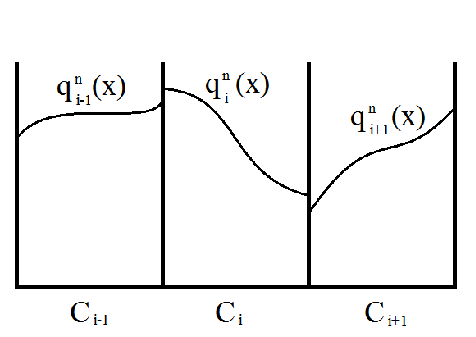
\includegraphics[angle=0,width=48mm]{FV/reconstruct.pdf} & 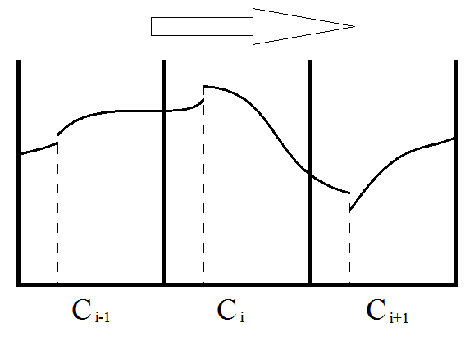
\includegraphics[angle=0,width=48mm]{FV/evolve.pdf} & 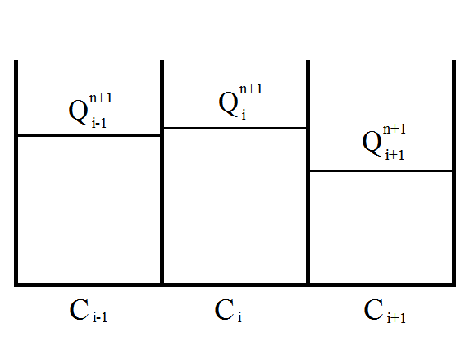
\includegraphics[angle=0,width=48mm]{FV/average.pdf}\\
{\small (1)} & {\small (2)} & {\small (3)}
\end{tabular}
\caption{REA algorithm with (1) Reconstruction phase, (2) evolution phase, and (3) cell averaging}
\end{figure}
\FloatBarrier
%%%%%%%%%%%%%%%%%%%%%%%%%%%%%%%%%%%%%%%%%%%%%%%%%%%%%%%%%%%%%%%%%%%%%%%%%%%%%%%
%%%%%%%%%%%%%%%%%%%%%%%%%%%%%%%%%%%%%%%%%%%%%%%%%%%%%%%%%%%%%%%%%%%%%%%%%%%%%%%
%%%%%%%%%%%%%%%%%%%%%%%%%%%%%%%%%%%%%%%%%%%%%%%%%%%%%%%%%%%%%%%%%%%%%%%%%%%%%%%
%%%%%%%%%%%%%%%%%%%%%%%%%%%%%%%%%%%%%%%%%%%%%%%%%%%%%%%%%%%%%%%%%%%%%%%%%%%%%%%
%%%%%%%%%%%%%%%%%%%%%%%%%%%%%%%%%%%%%%%%%%%%%%%%%%%%%%%%%%%%%%%%%%%%%%%%%%%%%%%
%%%%%%%%%%%%%%%%%%%%%%%%%%%%%%%%%%%%%%%%%%%%%%%%%%%%%%%%%%%%%%%%%%%%%%%%%%%%%%%
%%%%%%%%%%%%%%%%%%%%%%%%%%%%%%%%%%%%%%%%%%%%%%%%%%%%%%%%%%%%%%%%%%%%%%%%%%%%%%%
\subsection{CFL Condition For Stability}
A necessary condition for stability of FV methods, as well as FD methods, is the CFL condition. The CFL condition imposes a limit on the choice of the time step $\Delta t$ by the choice of the spatial step $\Delta x$. The CFL condition is defined by the relation
%
\begin{equation}
\label{CFLeq}
C = u \frac{\Delta t}{\Delta x}
\end{equation}
%
with some constraint on the constant $C$. This condition is attributed to Courant, Friedrich and Lewy \cite{cflCite}.

With the Godunov REA algorithm, the solutions in the cells will advect by some distance $u \Delta t$. See figure (\ref{CFLfig}). If this distance exceeds the cell length $\Delta x$, the cell values at the next time step will be influenced directly by cell values beyond the immediate neighboring cells. This effect is undesired because our methods depend on the flux from the neighboring cells. The resulting inequality is $u \Delta t \le \Delta x$. Rearranging terms and we obtain
%
\begin{equation*}
u \frac{\Delta t}{\Delta x} \le 1.
\end{equation*}
%
We find our constant to be $C = 1$ for the FV methods.
%Courant, Friedrich, and Lewy have shown that, by using finite difference methods they define a sequence of approximate solutions to certain PDE and shown that they converge and the limit must satisfy the PDE as the grid is refined. In LeVeque \cite{leveque} (pp. 69) The CFL condition is defined as: "A numerical method can be convergent only if its numerical domain of dependence contains the true domain of dependence of the PDE, at least in the limit as t and x go to zero." 
%
\begin{figure}[ht!]
  \centering
      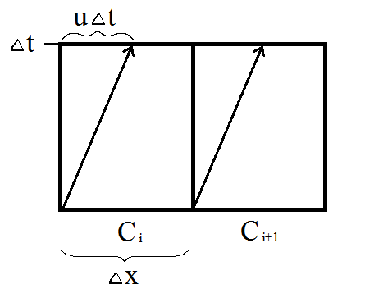
\includegraphics[angle=0,width=80mm]{CFL/cfl.pdf}
  \caption{after advection}
\label{CFLfig}
\end{figure}
\FloatBarrier
%
%The CFL condition is a necessary condition for both finite volume and finite difference methods for stability. For the transport equation, our gas advects from one cell to its neighbor after a time step of $\Delta t$ As can be seen in figure (\ref{CFLfig}). If the cell size $\Delta x$ is known, then the solution will advect a distance of $\Delta t u$. The finite volume methods we use will depend on neighboring cell values for the cell updates and so since $u$ is known the value of $\Delta t$ must be chosen such that $u \Delta t \le \Delta x$ or $u \Delta t = C \Delta x$ where $C <= 1$. Hence (\ref{CFLeq}).
%%%%%%%%%%%%%%%%%%%%%%%%%%%%%%%%%%%%%%%%%%%%%%%%%%%%%%%%%%%%%%%%%%%%%%%%%%%%%%%
%%%%%%%%%%%%%%%%%%%%%%%%%%%%%%%%%%%%%%%%%%%%%%%%%%%%%%%%%%%%%%%%%%%%%%%%%%%%%%%
%%%%%%%%%%%%%%%%%%%%%%%%%%%%%%%%%%%%%%%%%%%%%%%%%%%%%%%%%%%%%%%%%%%%%%%%%%%%%%%
%%%%%%%%%%%%%%%%%%%%%%%%%%%%%%%%%%%%%%%%%%%%%%%%%%%%%%%%%%%%%%%%%%%%%%%%%%%%%%%
%%%%%%%%%%%%%%%%%%%%%%%%%%%%%%%%%%%%%%%%%%%%%%%%%%%%%%%%%%%%%%%%%%%%%%%%%%%%%%%
%%%%%%%%%%%%%%%%%%%%%%%%%%%%%%%%%%%%%%%%%%%%%%%%%%%%%%%%%%%%%%%%%%%%%%%%%%%%%%%
%%%%%%%%%%%%%%%%%%%%%%%%%%%%%%%%%%%%%%%%%%%%%%%%%%%%%%%%%%%%%%%%%%%%%%%%%%%%%%%
%\section{First Order Approximation Method}
%In this section, we will derive the first order finite difference and finite volume methods and compare them. We will see that both methods are identical which will prove that the finite volume method we derive will be of first order accuracy.
%%%%%%%%%%%%%%%%%%%%%%%%%%%%%%%%%%%%%%%%%%%%%%%%%%%%%%%%%%%%%%%%%%%%%%%%%%%%%%%
%%%%%%%%%%%%%%%%%%%%%%%%%%%%%%%%%%%%%%%%%%%%%%%%%%%%%%%%%%%%%%%%%%%%%%%%%%%%%%%
%%%%%%%%%%%%%%%%%%%%%%%%%%%%%%%%%%%%%%%%%%%%%%%%%%%%%%%%%%%%%%%%%%%%%%%%%%%%%%%
%%%%%%%%%%%%%%%%%%%%%%%%%%%%%%%%%%%%%%%%%%%%%%%%%%%%%%%%%%%%%%%%%%%%%%%%%%%%%%%
\subsection{The First Order Finite Difference Method}
Let us derive the first order FD method for the transport equation. Recall the transport equation
%
\begin{equation}
\label{homoFirst}
\partial_t f(x,t) + u \partial_x f(x,t) = 0.
\end{equation}
%
A common practice for the derivation of FD methods stems from the Taylor series expansion. If $f$ is twice differentiable in time, then there exists $\xi_t \in [t,t+\Delta t]$ where
%
\begin{equation*}
f(x,t+\Delta t) = f(x,t) + \Delta t \partial_t f(x,t) + \frac{\Delta t^2}{2} \partial_t^2 f(x,\xi_t).
\end{equation*}
%
Writing the above equation in big O notation
%
\begin{equation*}
f(x,t+\Delta t) = f(x,t) + \Delta t \partial_t f(x,t) + O(\Delta t^2).
\end{equation*}
%
Similarly, if $f$ is twice differentiable in the $x$ variable, then we can approximate $f(x + \Delta x)$ by
%
\begin{equation*}
f(x + \Delta x,t) = f(x,t) + \Delta x \partial_x f(x,t) + O(\Delta x^2).
\end{equation*}
%
Notice that the dependence on the right nodal value ($x + \Delta x$) suggests we are solving for left moving waves $u<0$. Now from each of the expansions above, if we solve for $\partial_t f(x,t)$ and $\partial_x f(x,t)$ we obtain
%
\begin{align*}
&\partial_t f(x,t) = \frac{f(x,t+\Delta t) - f(x,t)}{\Delta t} + O(\Delta t)\\
&\partial_x f(x,t) = \frac{f(x+\Delta x,t) - f(x,t)}{\Delta x} + O(\Delta x)
\end{align*}
%
and substituting into (\ref{homoFirst}):
%
\begin{equation}
\label{dadada}
\left( \frac{f(x,t+\Delta t) - f(x,t)}{\Delta t} + O(\Delta t) \right) + u \left( \frac{f(x+\Delta x,t) - f(x,t)}{\Delta x} + O(\Delta x) \right) = 0.
\end{equation}
%
Solving for $f(x,t+\Delta t)$ from (\ref{dadada}):
%
\begin{equation*}
%\label{firstOrderHomo}
f(x,t+\Delta t) = f(x,t) - u \frac{\Delta t}{\Delta x} \left(f(x+\Delta x,t) - f(x,t)\right) + O(\Delta t^2) + O(\Delta x) \Delta t.
\end{equation*}
%
Recall from the CFL condition that $C \Delta x = u \Delta t$ and since $u$ is constant, $O(\Delta x) \Delta t = O(\Delta t^2)$ and so the above equation takes the form
%
\begin{equation}
\label{firstOrderHomoLeft}
f(x,t+\Delta t) = f(x,t) - u \frac{\Delta t}{\Delta x} \left(f(x+\Delta x,t) - f(x,t)\right) + O(\Delta t^2).
\end{equation}
%
The above equation is the first order FD method for solving (\ref{homoFirst}). Following the same process for right moving waves $u>0$, we obtain the equation using the left node ($x - \Delta x$)
%
\begin{equation}
\label{firstOrderHomoRight}
f(x,t+\Delta t) = f(x,t) - u \frac{\Delta t}{\Delta x} \left(f(x,t) - f(x - \Delta x,t)\right) + O(\Delta t^2).
\end{equation}
%%%%%%%%%%%%%%%%%%%%%%%%%%%%%%%%%%%%%%%%%%%%%%%%%%%%%%%%%%%%%%%%%%%%%%%%%%%%%%%
%%%%%%%%%%%%%%%%%%%%%%%%%%%%%%%%%%%%%%%%%%%%%%%%%%%%%%%%%%%%%%%%%%%%%%%%%%%%%%%
\subsection{The First Order Finite Volume Method}
We will now briefly derive the first order FV method. We start by employing Godunov's REA algorithm. Let $q_i^n(x) = Q_i^n$ be the constructed piecewise constant function approximating the solution at cell $C_i$ at time step $n$. During the time step the solutions are being transported to neighboring cells using the flux
%As we will see later, we can ignore the source term for now. We implement Godunov's method for linear systems by the reconstruct evolve average (REA) algorithm. This starts by reconstructing a polynomial approximation within a cell $C_i$ using the cell average, evolving the solution through time $\Delta t$, then developing the new cell average from which the process can be executed continuously over many time steps. For the first order approximation, Let's start with the assumption that our solution is piecewise constant in each cell. Given the velocity $u$ we can observe that the flux across the boundary through evolution will be given by
%
\begin{equation*}
\left\{
\begin{array}{cc}
F_{i-1/2}^n = u Q_{i-1}^n, & u>0\\
F_{i+1/2}^n = u Q_{i}^n, & u>0\\
F_{i-1/2}^n = u Q_{i}^n, & u<0\\
F_{i+1/2}^n = u Q_{i+1}^n, & u<0
\end{array}
\right.
\end{equation*}
%
where the direction of the flux depends on the sign of the velocity $u$. The new cell average is then determined as
%requires an addition from the incoming flux from the neighboring cell and subtracting off the flux lost to the other neighboring cell. So then evolving the solution at cell $C_i$ a time step $\Delta t$ later and averaging over the cell length $\Delta x$ our new cell averages become:
%
\begin{equation}
\label{first_order_FV_method}
\left\{
\begin{array}{cc}
Q_i^{n+1} = Q_i^n - u \frac{\Delta t}{\Delta x} (Q_{i}^n - Q_{i-1}^n), & u>0\\
Q_i^{n+1} = Q_i^n - u \frac{\Delta t}{\Delta x} (Q_{i+1}^n - Q_{i}^n), & u<0.
\end{array}
\right.
\end{equation}
%
Notice the above equations are the same as (\ref{firstOrderHomoLeft}) and (\ref{firstOrderHomoRight}) provided that the FD methods were derived using the function $f$ in the notation.
%Although the finite volume method is implemented for our use, we will observe that the first order finite difference approximation we obtain will yield the same result as the first order finite volume approach. This will also verify the first order accuracy of our FV method. This is not always the case as we will see later for a second order FV method.
%
%For the finite difference approximation consider the Taylor expansion of $f(x,t + \Delta t)$ through $t$ and $f(x + \Delta x,t)$ through $x$ for left moving waves:
%\begin{gather}
%\begin{aligned}
%\label{Taylor_expansion_1st_order}
%&f(x,t + \Delta t) = f(x,t) + \partial_t f(x,t) \Delta t + O(\Delta t^2)\\
%&f(x + \Delta x,t) = f(x,t) + \partial_x f(x,t) \Delta x + O(\Delta x^2)
%\end{aligned}
%\end{gather}
%
%Then the first derivative parts of each will be
%$$ \partial_x f(x,t) = \frac{f(x+\Delta x,t) - f(x,t)}{\Delta x} + O(\Delta x) $$
%$$ \partial_t f(x,t) = \frac{f(x,t+\Delta t) - f(x,t)}{\Delta t} + O(\Delta t) $$
%
%and by substituting this into (\ref{homoFirst}):
%$$ \left(\frac{f(x,t+\Delta t) - f(x,t)}{\Delta t} + O(\Delta t)\right) + \bar{u} \left(\frac{f(x+\Delta x,t) - f(x,t)}{\Delta x} + O(\Delta x)\right) = 0 $$ %\Psi (f(x,t))
%
%Then solving for $f(x,t+\Delta t)$:
%\begin{equation}
%f(x,t+\Delta t) = f(x,t) + \bar{u} \frac{\Delta t}{\Delta x} \left(f(x+\Delta x,t) - f(x,t)\right)% + \Delta t \Psi (f(x,t)) + O(\Delta t^2)
%\end{equation}
%
%Which is a first order accurate unsplit solution to $\ref{withSource}$. Note that by the CFL condition, a fixed $\Delta t$ is chosen so that $\Delta t = C \Delta x$ for some constant $C$ such that $0 < C \le \frac{1}{max(\bar{u_k}}$ then $O(\Delta x) = O(\Delta t)$. One can see the identical resemblance with \ref{first_order_FV_method}.
%%%%%%%%%%%%%%%%%%%%%%%%%%%%%%%%%%%%%%%%%%%%%%%%%%%%%%%%%%%%%%%%%%%%%%%%%%%%
%%%%%%%%%%%%%%%%%%%%%%%%%%%%%%%%%%%%%%%%%%%%%%%%%%%%%%%%%%%%%%%%%%%%%%%%%%%%
%%%%%%%%%%%%%%%%%%%%%%%%%%%%%%%%%%%%%%%%%%%%%%%%%%%%%%%%%%%%%%%%%%%%%%%%%%%%
%%%%%%%%%%%%%%%%%%%%%%%%%%%%%%%%%%%%%%%%%%%%%%%%%%%%%%%%%%%%%%%%%%%%%%%%%%%%
%%%%%%%%%%%%%%%%%%%%%%%%%%%%%%%%%%%%%%%%%%%%%%%%%%%%%%%%%%%%%%%%%%%%%%%%%%%%
%%%%%%%%%%%%%%%%%%%%%%%%%%%%%%%%%%%%%%%%%%%%%%%%%%%%%%%%%%%%%%%%%%%%%%%%%%%%
%%%%%%%%%%%%%%%%%%%%%%%%%%%%%%%%%%%%%%%%%%%%%%%%%%%%%%%%%%%%%%%%%%%%%%%%%%%%
%\section{Second Order Approximation Methods for the Advection Equation}
%In the first order advection method we assumed a piecewise constant solution for the advection problem and solved the source term using a first order forward Euler method. Similar to the first order method, our objective now is to develop a higher order method for the advection problem and for the source term. Because the fractional step method is only first order accurate, as shown before, our splitting method will employ Strang splitting. As long as the methods used for evolving the advection equation and the source term are both at least second order accurate then Strang splitting will guarantee that our combined solution will be at least second order accurate.
%%%%%%%%%%%%%%%%%%%%%%%%%%%%%%%%%%%%%%%%%%%%%%%%%%%%%%%%%%%%%%%%%%%%%%%%%%%%
%%%%%%%%%%%%%%%%%%%%%%%%%%%%%%%%%%%%%%%%%%%%%%%%%%%%%%%%%%%%%%%%%%%%%%%%%%%%
%%%%%%%%%%%%%%%%%%%%%%%%%%%%%%%%%%%%%%%%%%%%%%%%%%%%%%%%%%%%%%%%%%%%%%%%%%%%
%%%%%%%%%%%%%%%%%%%%%%%%%%%%%%%%%%%%%%%%%%%%%%%%%%%%%%%%%%%%%%%%%%%%%%%%%%%%
\subsection{The Second Order Finite Difference Method}
In this section, we will derive the second order FD method. The procedure is similar to the first order FD derivation except that second order terms are kept in the Taylor expansion. We start with the Taylor series expansion of $f(x,t+\Delta t)$ through time
%Since we observed that the first order FV method is identical to the first order FD method, it is only natural to question what makes the FV method different than the FD method. In this section we will derive the second order FD method and we will see that this is indeed a different result than the second order FV method. Then later we will show computed results showing that our FV method converges with second order accuracy.
%
\begin{equation*}
f(x,t+\Delta t) = f(x,t) + \Delta t \partial_t f(x,t) + \frac{\Delta t^2}{2} \partial_t^2 f(x,t) + O(\Delta t^3).
\end{equation*}
%
We want to derive a method to advance the solution a time step $\Delta t$. Because we don't have information about the solution through time but we do have information about the solution through $x$, we convert the time derivative terms in the above equation to the space derivative terms. By re-arranging (\ref{homoFirst}) in terms of $\partial_t f$
%
\begin{equation}
\label{firstPart}
\partial_t f = -u \partial_x f
\end{equation}
%
and also by the linearity of the differential operator
%
\begin{equation}
\label{secondPart}
\partial_t^2 f = \partial_t(\partial_t f) = \partial_t(-u \partial_x f) = -u \partial_x(\partial_t f) = -u \partial_x(-u \partial_x f) = u^2 \partial_x^2 f.
\end{equation}
%
%What we want to do here is since we are solving our system explicitly through time, we do not have information about the solution in the future time but we do have information about the solution through $x$ and so we can use (\ref{firstPart}) and (\ref{secondPart}) to replace the time derivatives of the Taylor expansion with the space derivative forms. This gives us
%
Using the above two relations, we replace the time derivative terms of the Taylor expansion by the spatial derivative terms
%
\begin{equation*}
f(x,t+\Delta t) = f(x,t) - u \Delta t \partial_x f(x,t) + u^2 \frac{\Delta t^2}{2} \partial_x^2 f(x,t) + O(\Delta t^3)
\end{equation*}
%
The central difference methods are then used to approximate the derivatives with second order accuracy:
%
\begin{align*}
f(x,t+\Delta t) =& f(x,t) - u \frac{\Delta t}{2 \Delta x} (f(x+\Delta x,t) - f(x-\Delta x,t))\\
&+ u^2 \frac{\Delta t^2}{2 \Delta x^2} (f(x-\Delta x,t) - 2 f(x,t) + f(x+\Delta x,t)) + O(\Delta t^3).
\end{align*}
%
The above is a second order accurate method to (\ref{homoFirst}). This is also known as the Lax–Wendroff method \cite{lax}.
%%%%%%%%%%%%%%%%%%%%%%%%%%%%%%%%%%%%%%%%%%%%%%%%%%%%%%%%%%%%%%%%%%%%%%%%%%%%
%%%%%%%%%%%%%%%%%%%%%%%%%%%%%%%%%%%%%%%%%%%%%%%%%%%%%%%%%%%%%%%%%%%%%%%%%%%%
%%%%%%%%%%%%%%%%%%%%%%%%%%%%%%%%%%%%%%%%%%%%%%%%%%%%%%%%%%%%%%%%%%%%%%%%%%%%
%%%%%%%%%%%%%%%%%%%%%%%%%%%%%%%%%%%%%%%%%%%%%%%%%%%%%%%%%%%%%%%%%%%%%%%%%%%%
\subsection{The Second Order Finite Volume Method}
We will derive the second order FV method for the transport equation using the same REA algorithm used for the first order FV method. The piecewise polynomial approximating the solution in cell $C_i$ at time $t_n$, in the first order FV method, used a constant polynomial equal to the cell average $Q_i$. In this section, we introduce a correction term to the piecewise polynomial by adding in a slope term $\sigma_i$. This slope is determined by an approximation to the derivative in $x$ by any conventional means. Let $q_i^n(x) = Q_i^n + \sigma_i (x - x_i)$ be the piecewise linear polynomial approximating the solution in cell $C_i$ at time $t_{n}$.
%Let us define $\mathring{q^n(x)}$ to be the exact solution at time step $n$ over the whole domain. We can better approximate the true solution everywhere in the domain if, in addition to the cell average at each cell, we approximate the slope of the solution. Let $Q_i$ refer to the cell average of at cell $C_i$ located at $x_i$. If we denote $\sigma_i$ to be the slope at cell $x_i$ then for all $x \in C_i$
%
%\begin{equation*}
%q_i^n(x) = Q_i^n + \sigma_i (x - x_i).
%\end{equation*}
%
%Notice that if our solution is smooth and if $q_i^n(x_i) = \mathring{q^n(x_i)}$ for each $i = 1,2,...,N$, then if our slope is approximated with at least second order accuracy then $q^n(x) - q_i^n(x) = O(\Delta x^2)$.
%
%There are two cases to look at. We can have advection to the right for positive moving waves $u>0$ or advection to the left for negative moving waves $u<0$. Since advection in one direction is the same process as in the other direction, we will observe positive velocities. referring to figure (), once we advect into cell $x_i$ the data is carried over by cell $Q_{i-1}$ ($Q_{i+1}$ if it's a left going wave). Note from figure (), if we advect to the right at some velocity $u$ then after some time $\Delta t$ the new cell average will be
%
%
%\begin{figure}[ht!]
%  \centering
%      \includegraphics[angle=0,width=140mm]{second_order/part1.jpg}
%  \caption{before advection}
%\label{before}
%\end{figure}
%%
%\begin{figure}[ht!]
%  \centering
%      \includegraphics[angle=0,width=140mm]{second_order/part2.jpg}
%  \caption{after advection}
%\label{after}
%\end{figure}
%\FloatBarrier
%
Let's derive the flux at the left boundary due to positive moving waves. Because we have a piecewise linear approximation at the left cell, the flux entering the cell from the left, $C_{i-1}$, is
%
\begin{align*}
%\label{FluxBoundaryLeft}
F_{i-1/2}^n &= \frac{1}{\Delta t} \int_{x_{i-1} + \frac{\Delta x}{2} - u \Delta t}^{x_{i-1} + \frac{\Delta x}{2}} q_{i-1}^n(x) dx \nonumber\\
&= \frac{1}{\Delta t} \int_{x_{i-1} + \frac{\Delta x}{2} - u \Delta t}^{x_{i-1} + \frac{\Delta x}{2}} Q_{i-1}^n + \sigma_{i-1}^n (x-x_{i-1}) dx \nonumber \\
&= \left( Q_{i-1}^n + \frac{\sigma_{i-1}^n}{2} (\Delta x - u \Delta t) \right) u
\end{align*}
%
and computing the flux leaving the cell $C_i$ at the right boundary is
%
\begin{align*}
%\label{FluxBoundaryRight}
F_{i+1/2}^n &= \frac{1}{\Delta t} \int_{x_i + \frac{\Delta x}{2} - u \Delta t}^{x_i + \frac{\Delta x}{2}} q_i^n(x) dx \nonumber\\
&= \frac{1}{\Delta t} \int_{x_i + \frac{\Delta x}{2} - u \Delta t}^{x_i + \frac{\Delta x}{2}} Q_i^n + \sigma_i^n (x-x_i) dx \nonumber\\
&= \left( Q_i^n + \frac{\sigma_{i}^n}{2} (\Delta x - u \Delta t) \right) u.
\end{align*}
%
Performing the same procedure to find the fluxes for left moving waves ($u<0$) and combining with the fluxes derived above provides the resulting fluxes
%
\begin{equation*}
\left\{
\begin{array}{cc}
F_{i-1/2}^n = \left( Q_{i-1}^n + \frac{\sigma_{i-1}^n}{2} (\Delta x - u \Delta t) \right) u, & u>0\\
F_{i+1/2}^n = \left( Q_i^n + \frac{\sigma_{i}^n}{2} (\Delta x - u \Delta t) \right) u, & u>0\\
F_{i-1/2}^n = \left( Q_{i}^n - \frac{\sigma_{i}^n}{2} (\Delta x + u \Delta t) \right) u, & u<0\\
F_{i+1/2}^n = \left( Q_{i+1}^n - \frac{\sigma_{i+1}^n}{2} (\Delta x + u \Delta t) \right) u, & u<0.
\end{array}
\right.
\end{equation*}
%
The new cell averages are obtained by implementing the above flux terms into (\ref{FVmethod})
%
\begin{equation}
\label{secondOrdFV}
\left\{
\begin{array}{cc}
Q_i^{n+1} = Q_i^n - \frac{u \Delta t}{\Delta x} (Q_i^n - Q_{i-1}^n) - \frac{1}{2} \frac{u \Delta t}{\Delta x} (\Delta x - u \Delta t) (\sigma_i^n - \sigma_{i-1}^n), \, & u > 0\\
Q_i^{n+1} = Q_i^n - \frac{u \Delta t}{\Delta x} (Q_{i+1}^n - Q_i^n) + \frac{1}{2} \frac{u \Delta t}{\Delta x} (\Delta x + u \Delta t) (\sigma_{i+1}^n - \sigma_i^n), \, & u < 0.
\end{array}
\right.
\end{equation}
%
%To find the solution at an arbitrary point $x \in X_i$ we make use of the slope $\sigma_i$ and the cell average which is also the center value $Q_i$ at time step $n$ we have:
%
%\begin{equation}
%\label{Qin}
%Q_i^n(x) = \sigma_i^n (x - x_{i-1})
%\end{equation}
%To get area 1 after advecting to the right, the right end point is $Q_{i-1}^n(x_{i-1}^n + \frac{\Delta x}{2})$ and the value at the left of area 1 is $Q_{i-1}^n(x_{i-1}+\frac{\Delta x}{2}-u \Delta t)$ and applying the same concept to get area 2 where we want to keep what is left of the cell and not has left. At the end, we arrive at the results of areas 1 and 2:
%\begin{equation}
%\label{Area1}
%A_1 = \frac{1}{2} (Q_{i-1}^n + \sigma_{i-1}^n (\frac{1}{2} \Delta x) + Q_{i-1}^n + \sigma_{i-1}^n (\frac{1}{2} \Delta %x - u \Delta t)) u \Delta t
%\end{equation}
%\begin{equation}
%\label{Area2}
%A_2 = \frac{1}{2} (Q_{i}^n + \sigma_i^n (-\frac{1}{2} \Delta x) + Q_{i-1}^n + \sigma_{i}^n (\frac{1}{2} \Delta x - u %\Delta t)) (\Delta x - u \Delta t)
%\end{equation}
%Then, the result final solution at cell $X_i$ at time step $n+1$ is
%$$ Q_i^{n+1} = (A_1 + A_2) \frac{1}{\Delta x} $$
%which comes out to be
%
%Then combining (\ref{FluxBoundaryLeft}) and (\ref{FluxBoundaryRight}) into (\ref{FVmethod}) we get
%\begin{equation}
%\label{Right}
%Q_i^{n+1} = Q_i^n - \frac{u \Delta t}{\Delta x} (Q_i^n - Q_{i-1}^n) - \frac{1}{2} \frac{u \Delta t}{\Delta x} (\Delta x - u \Delta t) (\sigma_i^n - \sigma_{i-1}^n), \, u > 0.
%\end{equation}
%
%Applying the same procedure for left moving waves we get
%
%\begin{equation}
%\label{Left}
%Q_i^{n+1} = Q_i^n - \frac{u \Delta t}{\Delta x} (Q_{i+1}^n - Q_i^n) + \frac{1}{2} \frac{u \Delta t}{\Delta x} (\Delta x + u \Delta t) (\sigma_{i+1}^n - \sigma_i^n), \, u < 0.
%\end{equation}
%
% R.LeVeques equation (6.13) on page 107
%Note that we have conserved the flux across the boundary yet we have introduced an additional correction term to our flux. Also,

The choice of the slope has no effect on the conservation of the method but if we let $\sigma = 0$ we will get the first order method back. The choice of the slope depends on the approximation of the derivative. For our case, we use the center difference slope which has an accuracy of $O(\Delta x^2)$
%
\begin{equation*}
%\label{CenterDiff}
\sigma_i^n = \frac{Q_{i+1}^n-Q_{i-1}^n}{2 \Delta x}.
\end{equation*}
%
Notice that the second order FV methods (\ref{secondOrdFV}) are not the same as the second order FD methods obtained earlier.
%%%%%%%%%%%%%%%%%%%%%%%%%%%%%%%%%%%%%%%%%%%%%%%%%%%%%%%%%%%%%%%%%%%%%%%%%
%To handle the right hand side, we split the problem into two parts. The first part is the homogeneous form of our PDE that we solve over one time step. Then the second part is of the form $q_t = B q$ which we solve for a half time step. The method we use starts by solving the B problem (as in R. LeVeques book) over a half time step then the A problem with a full time step then the B problem again with a half time step. (page 387 explains why this preserves higher order accuracy) which is known as Strang Splitting. Since we do not have information about the derivative, we can get second order accuracy with the second order Runge Kutta method for the B step.
%%%%%%%%%%%%%%%%%%%%%%%%%%%%%%%%%%%%%%%%%%%%%%%%%%%%%%%%%%%%%%%%%%%%%%%%%%%%%%%
%%%%%%%%%%%%%%%%%%%%%%%%%%%%%%%%%%%%%%%%%%%%%%%%%%%%%%%%%%%%%%%%%%%%%%%%%%%%%%%
\subsection{Two Step Runge Kutta for the Collision Operator of the Kinetic Models}
The use of a splitting method described in the next section, the solution to the model kinetic equation can be done by advancing the transport and the collision part of the equations in alternating fashion. Thus in the first step one solves the transport equation using either the first or second order techniques. In the second step, the collision part of the model equation if solved in one temporal interval.
%
\begin{equation}
\label{2271}
\partial_t f(x,t) = \Psi(f).
\end{equation}
%
In case when analytical solution is not available and the equation needs to be solved numerically, the order of accuracy for the time integration has to be consistent with the desired order of the splitting technique. In particular, if the first order splitting technique is sought, then the scheme advancing (\ref{2271}) in time should be first order and if second order splitting is desired, then second order time integration should be used to advance solution to (\ref{2271}) in time. In the case of the first order splitting, one can use Euler's method to discretize (\ref{2271}) in time. In the case of second order splitting, a second order time discretization scheme needs to be proposed. In this approach we do not have the convenience of trading derivatives used in the derivation of second order method (\ref{firstPart})-(\ref{secondPart}). Instead, to achieve second order accuracy we apply a two-stage Runge-Kutta method. Namely,
%
\begin{align*}
k_1 &= Q_i + \frac{\Delta t}{2} \Psi(f,t_n)\\
Q_i^{n+1} &= Q_i^n + \Delta t \Psi(k_1,t_n + \Delta t/2).
\end{align*}
%%%%%%%%%%%%%%%%%%%%%%%%%%%%%%%%%%%%%%%%%%%%%%%%%%%%%%%%%%%%%%%%%%%%%%%%%%%%
%%%%%%%%%%%%%%%%%%%%%%%%%%%%%%%%%%%%%%%%%%%%%%%%%%%%%%%%%%%%%%%%%%%%%%%%%%%%
%%%%%%%%%%%%%%%%%%%%%%%%%%%%%%%%%%%%%%%%%%%%%%%%%%%%%%%%%%%%%%%%%%%%%%%%%%%%
%%%%%%%%%%%%%%%%%%%%%%%%%%%%%%%%%%%%%%%%%%%%%%%%%%%%%%%%%%%%%%%%%%%%%%%%%%%%
%%%%%%%%%%%%%%%%%%%%%%%%%%%%%%%%%%%%%%%%%%%%%%%%%%%%%%%%%%%%%%%%%%%%%%%%%%%%
%%%%%%%%%%%%%%%%%%%%%%%%%%%%%%%%%%%%%%%%%%%%%%%%%%%%%%%%%%%%%%%%%%%%%%%%%%%%
%%%%%%%%%%%%%%%%%%%%%%%%%%%%%%%%%%%%%%%%%%%%%%%%%%%%%%%%%%%%%%%%%%%%%%%%%%%%
\section{Splitting Methods}
In this section we discuss the splitting methods for splitting the BGK and ES-BGK kinetic models of the form
%
\begin{equation}
\label{kineticModel}
\partial_t f + u \, \partial_x f = \Psi (f).
\end{equation}
%
Obviously, the FV methods discussed will not solve the above equation directly. Instead, the FV methods solve the homogeneous transport equation
%
\begin{equation}
\label{homo}
\partial_t f + u \partial_x f = 0.
\end{equation}
%
To include the source term, we make use of the solution to the ODE describing $f$ along the characteristic curve of (\ref{kineticModel}) namely
%
\begin{equation}
\label{char}
\frac{df}{dt} = \Psi (f).
\end{equation}
%
Along the characteristic ($dx/dt = u$), the homogeneous equation remains constant through time. For this reason, we advance the solution to (\ref{kineticModel}) through time by advancing the transport equation through time then update the solution by advancing (\ref{char}). This is the idea behind the splitting methods.
%In many cases, solving the kinetic equations directly may be more difficult than if we were to solve the homogeneous form first then solve along the characteristic which can be expressed as a simple ODE. Here we will derive splitting methods that will allow us to solve for $f$ with first order accuracy and for higher accuracy.
%%%%%%%%%%%%%%%%%%%%%%%%%%%%%%%%%%%%%%%%%%%%%%%%%%%%%%%%%%%%%%%%%%%%%%%%%%%%
%%%%%%%%%%%%%%%%%%%%%%%%%%%%%%%%%%%%%%%%%%%%%%%%%%%%%%%%%%%%%%%%%%%%%%%%%%%%
%%%%%%%%%%%%%%%%%%%%%%%%%%%%%%%%%%%%%%%%%%%%%%%%%%%%%%%%%%%%%%%%%%%%%%%%%%%%
\subsection{Fractional Step Method}
The fractional step method allows us to perform first order splitting of (\ref{kineticModel}).
%leveque - why this is only first order accurate
%R. LeVeque page 380
In R. LeVeque \cite{leveque}, it is claimed that if we solve for (\ref{homo}) with first order accuracy over a whole time step $\Delta t$ then use that intermediate value to advance (\ref{char}) over a whole time step with first order accuracy, then we will have solved (\ref{kineticModel}) over a whole time step with first order accuracy in both $x$ and $t$. We will briefly verify this claim. Consider the unsplit form (\ref{kineticModel}). Let us update our solution over a time step of $\Delta t$ for left going waves $u<0$ (right going waves follow the same procedure) by
%
\begin{equation}
\label{firstOrderUnsplit}
f(x,t+\Delta t) = f(x,t) + \bar{u} \frac{\Delta t}{\Delta x} \left(f(x+\Delta x,t) - f(x,t)\right) + \Delta t \Psi(f(x,t)) + O(\Delta t^2).
\end{equation}
%

Now, consider that we update our solution by first advancing (\ref{homo}) by a time step $\Delta t$ from the above equation and call it $f^*(x,t)$. Then use the forward Euler approximation of the time evolution of (\ref{char}). We would then have a two step form process of the numerical solution as follows
%
\begin{align*}
\text{step A}& \quad f^*(x,t) = \left\{ \begin{array}{cl} f(x,t) + u \frac{\Delta t}{\Delta x} \left(f(x+\Delta x,t) - f(x,t)\right) & u<0\\
f(x,t) + u \frac{\Delta t}{\Delta x} \left(f(x,t) - f(x - \Delta x,t)\right) & u>0 \end{array} \right.\\
\text{step B}& \quad f(x,t+\Delta t) = f^*(x,t) + \Delta t \Psi(f^*(x,t)).
\end{align*}
%
We can see that by substituting the result from Step A directly into step B we get something similar to the unsplit method with the only difference being that the $\Psi(f(x,t))$ term in the unsplit method is replaced by the $\Psi(f^*(x,t))$ term. We can see from (\ref{firstOrderUnsplit}) that $f^*(x,t) = f(x,t) + O(\Delta t)$ and so
%
\begin{align*}
\Psi(f^*(x,t)) &= \Psi \left(f(x,t) + O(\Delta t) \right)\\
&= \Psi \left(f(x,t) \right) + O(\Delta t)
\end{align*}
%
giving us the expanded form (for left moving waves $u<0$)
%
\begin{equation*}
f(x,t+\Delta t) = f(x,t) + \bar{u} \frac{\Delta t}{\Delta x} \left(f(x+\Delta x,t) - f(x,t)\right) + \Delta t \Psi(f(x,t)) + O(\Delta t^2)
\end{equation*}
%
We notice that the form of this expression agrees with the unsplit method at the same level of accuracy. It may appear as if we have advanced the solution by two time steps, but we have advected the solution then updated the solution from the source term. This splitting technique is limited to first order approximation and a different technique for higher order accuracy will be looked at next.
%%%%%%%%%%%%%%%%%%%%%%%%%%%%%%%%%%%%%%%%%%%%%%%%%%%%%%%%%%%%%%%%%%%%%%%%%%%%%%%
%%%%%%%%%%%%%%%%%%%%%%%%%%%%%%%%%%%%%%%%%%%%%%%%%%%%%%%%%%%%%%%%%%%%%%%%%%%%%%%
%%%%%%%%%%%%%%%%%%%%%%%%%%%%%%%%%%%%%%%%%%%%%%%%%%%%%%%%%%%%%%%%%%%%%%%%%%%%%%%
%%%%%%%%%%%%%%%%%%%%%%%%%%%%%%%%%%%%%%%%%%%%%%%%%%%%%%%%%%%%%%%%%%%%%%%%%%%%%%%
%%%%%%%%%%%%%%%%%%%%%%%%%%%%%%%%%%%%%%%%%%%%%%%%%%%%%%%%%%%%%%%%%%%%%%%%%%%%%%%
%%%%%%%%%%%%%%%%%%%%%%%%%%%%%%%%%%%%%%%%%%%%%%%%%%%%%%%%%%%%%%%%%%%%%%%%%%%%%%%
%%%%%%%%%%%%%%%%%%%%%%%%%%%%%%%%%%%%%%%%%%%%%%%%%%%%%%%%%%%%%%%%%%%%%%%%%%%%%%%
\subsection{Linear Strang Splitting}
The fractional step method will give first order accuracy as long as (\ref{homo}) and (\ref{char}) are first order accurate. Unfortunately, it will not provide second order or above accuracy no matter how accurate the methods used in the solution of Step A and Step B are. To compensate for this, Strang splitting is introduced where the solution can be computed over different sized time steps. In Strang \cite{strang} linear equations with operators $A$ and $B$ of the form
%
\begin{equation}
\label{linearEq}
\partial_t f = A f + B f
\end{equation}
%
have the exact solution of the form
%
\begin{equation}
f(x,t_0 + \Delta t) = e^{\Delta t (A + B)}f(x,t_0).
\end{equation}
%
Rather than solving (\ref{linearEq}) directly, one solves the equations
%
\begin{equation}
\label{partA}
\partial_t f = A f
\end{equation}
%
and
%
\begin{equation}
\label{partB}
\partial_t f = B f
\end{equation}
%
while keeping the solution $f$ updated in time in the order they are evaluated. In the case that the operators $A$ and $B$ are commutable, this is as simple as solving (\ref{partA}) with a whole time step. Indeed, in this case, $f(x,t_0 + \Delta t) = e^{\Delta t A}e^{\Delta t B} f(x,t_0) = e^{\Delta t (A + B)} f(x,t_0)$. However, in general, operators $A$ and $B$ do not commute. Strang (1968) \cite{strang} has proposed to solve (\ref{partA}) over a half time step. Use the result in (\ref{partB}) over a whole time step. Then use that result in (\ref{partA}) again over a half time step. The result will be second order accurate provided that each of the steps are at least second order accurate. The combined result of the three steps can be written as
%
\begin{equation}
\label{Strang2}
f(x,t_0+\Delta t) \approx e^{\frac{\Delta t}{2} A} e^{\Delta t B} e^{\frac{\Delta t}{2} A} f(x,t_0).
\end{equation}
%
\begin{figure}[h!]
  \centering
      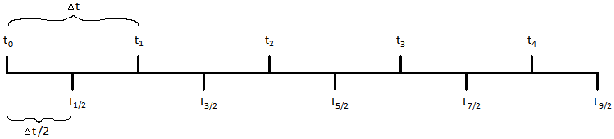
\includegraphics[angle=0,width=150mm]{strang/strang.pdf}
  \caption{\label{strang_interval} The top marks illustrate the time steps for the fractional step method. The bottom marks illustrate the time steps for the Strang splitting. The solution to the kinetic model equation is advanced a whole time step at every $t_{2n}$ for $n=1,2,3,...$.}
\end{figure}
\FloatBarrier
%
Expanding out each of the exponents of the RHS of (\ref{Strang2}) through Taylor series and multiplying together we get
%
\begin{align*}
e^{\frac{\Delta t}{2} A} e^{\Delta t B} e^{\frac{\Delta t}{2} A} &= 1 + \Delta t \left(\frac{1}{2} A + B + \frac{1}{2} A\right)\\
&+ \Delta t^2 \left(\frac{1}{8} A^2 + \frac{1}{2} A B + \frac{1}{2} B^2 + \frac{1}{4} A^2 + \frac{1}{2} B A + \frac{1}{8} B^2 \right) + O(\Delta t^3)\\
&= 1 + \Delta t (A + B) + \frac{\Delta t^2}{2}(A + B)^2 + O(\Delta t^3).
\end{align*}
%
Preserving the second order accuracy of the method.
%%%%%%%%%%%%%%%%%%%%%%%%%%%%%%%%%%%%%%%%%%%%%%%%%%%%%%%%%%%%%%%%%%%%%%%%%%%%%%%
%%%%%%%%%%%%%%%%%%%%%%%%%%%%%%%%%%%%%%%%%%%%%%%%%%%%%%%%%%%%%%%%%%%%%%%%%%%%%%%
%%%%%%%%%%%%%%%%%%%%%%%%%%%%%%%%%%%%%%%%%%%%%%%%%%%%%%%%%%%%%%%%%%%%%%%%%%%%%%%
%%%%%%%%%%%%%%%%%%%%%%%%%%%%%%%%%%%%%%%%%%%%%%%%%%%%%%%%%%%%%%%%%%%%%%%%%%%%%%%
%%%%%%%%%%%%%%%%%%%%%%%%%%%%%%%%%%%%%%%%%%%%%%%%%%%%%%%%%%%%%%%%%%%%%%%%%%%%%%%
%%%%%%%%%%%%%%%%%%%%%%%%%%%%%%%%%%%%%%%%%%%%%%%%%%%%%%%%%%%%%%%%%%%%%%%%%%%%%%%
\subsection{Non-Linear Strang Splitting}
In many applications where high resolution methods are desired for linear equations, Strang splitting is guaranteed to work. Here, we will show that Strang splitting will still give us second order accuracy for nonlinear systems of equations given that each step is at least second order accurate. Jianke Yang \cite{yang} (page 336-340) has shown that nonlinear Strang splitting methods will work up to fourth order accuracy. This is important to consider since in the case of the kinetic models used, the right hand side of the BGK and ES-BGK equations are a nonlinear operators. The set up for the nonlinear methods will be the same as with the linear methods. Consider ($\ref{linearEq}$) but now replace the linear operators $A$ and $B$ with the non-linear operators $M$ and $N$ so that the general equation is of the form of
\begin{equation}
\label{nonLinearEq}
\partial_t f = M(f) + N(f).
\end{equation}
%
We will split ($\ref{nonLinearEq}$) into two parts to be integrated separately, namely
\begin{equation}
\label{part1}
\partial_t f = M(f)
\end{equation}
%
and
\begin{equation}
\label{part2}
\partial_t f = N(f).
\end{equation}
%
The idea here is to evaluate the integral of the first equation (\ref{part1}) over a half time step. Use that result to then advance the solution in the second equation (\ref{part2}) over a whole time step. Then use this result again in a half time step evolution in the first equation. By repeating this process we can see that the last step is evaluated again over a half time step and so we can evaluate both components over a whole time step but offset by $\frac{\Delta t}{2}$ suggesting a similarity to the fractional step method. Because of the symmetric structure of (\ref{nonLinearEq}) we choose  to associate with the first step does not matter. However, to be specific, let us first start with (\ref{part1}). Just like with the linear Strang splitting, we will proceed to integrate ($\ref{part1}$) over a half time step $\frac{\Delta t}{2}$ from $t_0$ and designate this result with $f^*$
%
\begin{equation}
\label{v1}
f^* = f(x,t_0) + M(f(x,t_0)) \frac{\Delta t}{2} + \nabla M(M(f(x,t_0))) \frac{\Delta t^2}{8} + O(\Delta t^3).
\end{equation}
%
We then integrate ($\ref{part2}$) over a whole time step $\Delta t$ starting at $f^*$ and designate the next result with $f^{**}$.
%
\begin{equation}
\label{v2}
f^{**} = f^* + N(f^*) \Delta t + \frac{\Delta t^2}{2} \nabla N(N(f^*)) + O(\Delta t^3).
\end{equation}
%
Notice that
%
\begin{equation}
\label{Nv1}
N(f^*) = N \left(u_0 + \frac{1}{2} M \Delta t + O(\Delta t^2)\right) = N(f_0) + \frac{1}{2} \nabla N(M(f_0)) \Delta t + O(\Delta t^2)
\end{equation}
%
and
%
\begin{equation}
\label{NNv1}
\nabla N\left(N(f^*)\right) = \nabla N \left(N(f_0) + \frac{1}{2} \nabla N(M(f_0)) \Delta t + O(\Delta t^2) \right) = \nabla N\left(N(f_0)\right) + O(\Delta t)
\end{equation}
%
we substitute (\ref{v1}) into (\ref{v2}) and expand the result to the form
%
\begin{equation}
f^{**} = f_0 + \left(\frac{1}{2} M + N \right) \Delta t + \frac{1}{2} \left[ \frac{1}{4} \nabla M\left(M \right) + \nabla N\left(M+N \right)\right] \Delta t^2 + O(\Delta t^3).
\end{equation}
%
At the final step, we evaluate ($\ref{part1}$) over a half time step $\frac{\Delta t}{2}$ starting from our latest solution $f^{**}$ to get
%
\begin{equation}
\label{fss}
f(x,t_0+\Delta t) = f^{**} + \frac{1}{2} M(f^{**}) \Delta t + \frac{1}{8} \nabla M \left( M(f^{**}) \right) \Delta t^2 + O(\Delta t^3).
\end{equation}
%
If we expand the $M(f^{**})$ term we see that
%
\begin{equation}
\label{Mfss}
M(f^{**}) = M\left(f_0 + \left(\frac{1}{2}M + N \right) \Delta t + O(\Delta t^2)\right) = M + \nabla M(\frac{1}{2} M + N) \Delta t + O(\Delta t^2)
\end{equation}
%
and so
%
\begin{equation}
\label{MMfss}
\nabla M \left(M(f^{**})\right) = \nabla M\left(M + O(\Delta t)\right) = \nabla M\left(M \right) + O(\Delta t).
\end{equation}
%
Substituting (\ref{Mfss}) and (\ref{MMfss}) into (\ref{fss}) we get
%
\begin{equation*}
f(x,t+\Delta t) = f_0 + \left(\frac{1}{2} M + N \right) \Delta t + \frac{1}{2} \left[ \frac{1}{4} \nabla M \left(M \right) + \nabla N\left (M + N \right) \right] \Delta t^2
\end{equation*}
\begin{equation*}
 + \frac{1}{2} \left[M + \nabla M(\frac{1}{2} M + N) \Delta t \right] \Delta t + \frac{1}{8} \nabla M(M) \Delta t^2 + O(\Delta t^3).
\end{equation*}
%
After simplification,
%
\begin{equation}
f(x,t+\Delta t) = f_0 + \left(M + N\right) \Delta t + \frac{1}{2} \left[ \nabla (M + N)(M + N) \right] \Delta t^2 + O(\Delta t^3).
\end{equation}
%
%Now, $N(v_1) = N(u_0 + \zeta) = N(u_0) + N_t (u_0) \zeta + O(\zeta^2)$ where $\zeta = M(u_0) \frac{h}{2} + M_t(u_0) \frac{h^2}{8} + O(h^3)$ and consequently $O(\zeta) = O(h)$ So then
%
%$$ N(v_1) = N(u_0) + N_t(u_0) \left(M(u_0) \frac{h}{2} + M_t(u_0) \frac{h^2}{8}\right) + O(h^3) $$
%
%$$ N(v_1) = N(u_0) + N_t(u_0) M(u_0) \frac{h}{2} + N_t(u_0) M_t(u_0) \frac{h^2}{8} + O(h^3) $$
%
%$$ N_t (v_1) = N(u_0) + O(h) $$
%then substituting into the $v_2$ equation
%
%$$
%v_2 = v_1 + N(u_0) h + N_t(u_0) M(u_0) \frac{h^2}{2} + N_t(u_0) M_t(u_0) \frac{h^3}{8} + \frac{h^2}{2} N_t (v_1) + O(h^3)
%$$
%%%%%%%%%%%%%%%%%%%%%%%%%%%%%%%%%%%%%%%%%%%%%%%%%%%%%%%%%%%%%%%%%%%%%%%%%%%%%%%
This is a general formulation for nonlinear equations. For our implementation, we will have $M(f) = \nu (f_0 - f)$, the relaxation term, and $N(f) = -\partial_x f$, the differential operator through $x$ operated on f. For our system the $N(f)$ term is linear but the $M(f)$ term is nonlinear. We implement Strang splitting for the second order solver in the CLAWPACK software package.

\chapter{CLAWPACK}
CLAWPACK is a software package developed in Fortran by LeVeque et al \cite{clawly} for the solution of hyperbolic PDEs in one and two spatial dimensions. It is explicit in time and supports first and second order accurate schemes. Flux limiters are also supported for solving problems with discontinuities but because we do not deal with discontinuities, we do not use limiters in our implementation. Implementations of CLAWPACK include Geo-claw for Tsunami modeling and other geophysical flows. In this thesis we extend CLAWPACK to the solution of the model kinetic equations of the Boltzmann equation.

We notice that CLAWPACK is capable of handling multicomponent systems of hyperbolic equations including the BGK and ES-BGK kinetic models. Therefore its extension to the kinetic solutions only requires adding components that perform discretization in the velocity space and adding components for evaluation of the discrete collision operator. Also, CLAWPACK requires that a Riemann solver for the hyperbolic systems be provided.

Time integration in CLAWPACK utilizes the splitting technique. As discussed earlier, we solve the homogeneous transport equation and its collision operator separately.

Both first order and second order Riemann solvers are implemented. The fractional step method is used for the first order method and Strang splitting is used for the second order method.

\chapter{Experimental Results}
The CLAWPACK software was used to carry out simulations of the one-dimensional heat transfer problem and the normal shock wave problem with the BGK and ES-BGK models.

In the first section, we solve the homogeneous transport equation. This simulation was used to verify the first and second order accuracy of the first and second order FV methods respectively. We start with a Gaussian profile and allow the profile to move with time. The $L_1$ error is computed against the exact solution. Computation time for the first and second order methods were compared.

In the heat transfer problem, we simulate process of exchange of energy in Nitrogen gas enclosed between two infinitely long parallel plates. Each of the plates are uniformly heated at constant temperatures. The initial state of the gas is uniform everywhere between the plates. Therefore, there are no changes in the state of the gas in the directions parallel to the plates. We show that our numerical method conserves mass velocity discretizations. Momentum of the solution was shown to be near zero when the solution approaches steady state.

In the shock wave problem, we simulate motion of Argon gas in an open system. The gas is allowed to flow into the system at a constant rate upstream of the gas. The gas is then allowed to leave the system downstream at a constant rate determined by the Rankine-Hugoniot relations \cite{roshko} and the upstream conditions. Somewhere between the upstream and downstream boundaries, a shock wave is formed. We compute numerical solutions to the shock wave problem computed using the BGK and the ES-BGk models and and compare the numerical results to the experimental results of Alsmeyer's \cite{alsmeyer} Specifically, we compare the density and temperature profiles and the reciprocal shock thickness which we will later. Mass flow rate, momentum and energy results are shown to be conserved. Order of convergence was obtained for both the first order and second order simulations.

%and the shock-wave with a constant steady upstream and downstream flow. In our first observation we will look at the steady state results of the heat transfer between two infinitely long parallel plates. Then we will observe the results of the simulated shock-wave simulation with Mach numbers ranging from $1.20$ to $9.00$ where the reciprocal shock thickness are compared to Alsmeyer's \cite{alsmeyer} results. In addition, mass, momentum and energy results are shown to be conserved. First and second order FV methods are shown to converge with their respective orders of convergence. An absolute convergence to a known quantity is observed for the homogeneous case and the relative convergence is analyzed for the whole solution.
%
%\begin{equation}
%\label{f2Part}
%\partial_t f_2 + u_1 \partial_x f_2 = \nu \left( \int_{\mathbb{R}^2} u_2^2 f_0 du_2 du_3 - f_2 \right)
%\end{equation}
%
%%%%%%%%%%%%%%%%%%%%%%%%%%%%%%%%%%%%%%%%%%%%%%%%%%%%%%%%%%%%%%%%%%%%%%%%%%%%
%%%%%%%%%%%%%%%%%%%%%%%%%%%%%%%%%%%%%%%%%%%%%%%%%%%%%%%%%%%%%%%%%%%%%%%%%%%%
%%%%%%%%%%%%%%%%%%%%%%%%%%%%%%%%%%%%%%%%%%%%%%%%%%%%%%%%%%%%%%%%%%%%%%%%%%%%
%%%%%%%%%%%%%%%%%%%%%%%%%%%%%%%%%%%%%%%%%%%%%%%%%%%%%%%%%%%%%%%%%%%%%%%%%%%%
%%%%%%%%%%%%%%%%%%%%%%%%%%%%%%%%%%%%%%%%%%%%%%%%%%%%%%%%%%%%%%%%%%%%%%%%%%%%
%%%%%%%%%%%%%%%%%%%%%%%%%%%%%%%%%%%%%%%%%%%%%%%%%%%%%%%%%%%%%%%%%%%%%%%%%%%%
%%%%%%%%%%%%%%%%%%%%%%%%%%%%%%%%%%%%%%%%%%%%%%%%%%%%%%%%%%%%%%%%%%%%%%%%%%%%
\section{Homogeneous Transport Experiment}
In this section we will verify the accuracy of the implemented temporal and spatial discretizations of the kinetic equations by solving the homogeneous transport part and comparing the results to an exact solution. Consider the one dimensional homogeneous transport equation
%
\begin{equation}
\label{transport}
\partial_{t} f + u\, \partial_{x} f = 0.
\end{equation}
%
An exact solution to (\ref{transport}) is given by $f(x,t) = \mathring{f}(x - u t)$, where $\mathring{f}(\xi)$ is an arbitrary differentiable function of variable $\xi$. Equation \ref{transport} is solved numerically on the interval $x \in [-20,20]$ with the initial data given by the Gaussian profile
%
\begin{equation}
\mathring{f}(x)= \frac{1}{m \sqrt{\pi}}\exp \left( \frac{-(x-x_{0})^2}{m^2} \right),
\end{equation}
%
where the value of the normalizing constant $m=2.04$ is selected to guarantee that the profile is well contained in the domain. The value of the velocity $u$ is about $1000$ m/s which is on the same order of magnitude as the velocity values used in simulations of the model kinetic equations. Numerical solutions are computed for up to time $t = 0.008$ seconds. In Table~\ref{ErrorConvergence} the values of the $L_{1}$ and $L_{\infty}$ relative errors are presented for different numbers of spatial cells, $N$. Here $\|e\|_{L_{1}}$ and $\| e \|_{L_{\infty}}$ denote the values of $L_{1}$ and $L_{\infty}$ errors with respect to the exact solution, correspondingly, and $\alpha$ is the estimated order of convergence. The corresponding CPU time is shown in Figure~\ref{fig:CPU_time}
%
\begin{table}[!htb]
\centering
\begin{tabular*}{0.75\textwidth}{| c | c   c   c   c | c   c   c   c |} 
\cline{1-9}
& \multicolumn{4}{| c |}{First order} & \multicolumn{4}{| c |}{Second order}\\ 
%\cline{1-9}
$N$ & $\|e\|_{L_{1}}$ & $\alpha$ & $\| e \|_{L_{\infty}}$ & $\alpha$ & $\|e\|_{L_{1}}$ & $\alpha$ &  $\| e \|_{L_{\infty}}$ & $\alpha$\\ \cline{1-9}
%100 & 1.3E-1 & .92 & 1.3E-1 & .88 & 8.305E-3 & 2.3 & 1.4E-2 & 2.4\\
200 & 6.9E-2 & .94 & 7.1E-2 & .94 & 1.754E-3 & 2.1 & 2.7E-2 & 5.8\\
%300 & 4.7E-2 & .96 & 4.9E-2 & .96 & 7.45E-4 & 2.0 & 9.8E-4 & 2.6\\
400 & 3.6E-2 & 1.0 & 3.7E-2 & .97 & 4.12E-4 & 2.1 & 4.7E-4 & 2.7\\
%500 & 2.9E-2 & .97 & 3.0E-2 & .97 & 2.61E-4 & 2.1 & 2.6E-4 & 2.8\\
600 & 2.4E-2 & 1.0 & 2.5E-2 & .95 & 1.79E-4 & 2.0 & 1.6E-4 & 3.2\\
%700 & 2.1E-2 & .98 & 2.1E-2 & .98 & 1.32E-4 & 2.0 & 9.8E-5 & 3.2\\
800 & 1.8E-2 & 1.0 & 1.9E-2 & .94 & 1.01E-4 & 2.1 & 6.4E-5 & 3.9\\
1200 & 1.2E-2 &  & 1.3E-2 & & 4.36E-5 &  & 1.3E-5 &\\ \cline{1-9}
\end{tabular*}
\vspace*{5mm}
\caption{\label{ErrorConvergence} Values of $L_{1}$ and $L_{\infty}$ relative errors in the solution to the homogeneous transport equation for different numbers of spatial cells, $N$, and the estimated order of convergence, $\alpha$.}
\end{table}
\FloatBarrier
%
\begin{figure}[here]
\centering
\includegraphics[height=.35\textheight]{second_order/CPU_time.pdf}
\caption{Comparison of the CPU times for the solution of the transport equation using first order and second order FV schemes.}
\label{fig:CPU_time}
\end{figure}
%
Table~(\ref{ErrorConvergence}) shows that both $L_1$ and $L_\infty$ errors converge with the expected order for the used finite volume discretization. It appears that the convergence of the $L_\infty$ norm is faster than second order in the case of the second order FV scheme. For high resolutions, it accelerates almost to order four. However, we believe that this is just an artifact specific to the Gaussian profile and we do not expect this to hold for other exact solutions. It is apparent from Table~(\ref{ErrorConvergence}) and Figure~(\ref{fig:CPU_time}) that the second order FV method is significantly closer to the true solution with little difference in computation time. Therefore, in these simulations the second order method is preferable. As it  will be evident further, a similar conclusion holds for the first and second order FV discretization of the full model equations in the case of the normal shock wave problem.
%%%%%%%%%%%%%%%%%%%%%%%%%%%%%%%%%%%%%%%%%%%%%%%%%%%%%%%%%%%%%%%%%%%%%%%%%%%%%
%%%%%%%%%%%%%%%%%%%%%%%%%%%%%%%%%%%%%%%%%%%%%%%%%%%%%%%%%%%%%%%%%%%%%%%%%%%%%
%%%%%%%%%%%%%%%%%%%%%%%%%%%%%%%%%%%%%%%%%%%%%%%%%%%%%%%%%%%%%%%%%%%%%%%%%%%%%
%%%%%%%%%%%%%%%%%%%%%%%%%%%%%%%%%%%%%%%%%%%%%%%%%%%%%%%%%%%%%%%%%%%%%%%%%%%%%
%%%%%%%%%%%%%%%%%%%%%%%%%%%%%%%%%%%%%%%%%%%%%%%%%%%%%%%%%%%%%%%%%%%%%%%%%%%%%
\section{Boundary Conditions}
The standard approach to the solution of symmetric hyperbolic systems is to specify boundary conditions for incoming characteristic nodes. In our case, the left and right boundary conditions need to be specified for components of $h_{p,i}$ and $g_{p,i}$ that correspond to the incoming velocity nodes $u_{p,i}$.
%and on the right boundary the conditions have to be specified for components corresponding to negative velocity nodes $u_{p,i}$.

Two types of boundary conditions corresponding to two different flow conditions will be used. The first case arises in the problem of heat transfer where the gas is contained between two infinitely long parallel plates. the fact that the gas is trapped between the plates implies that the total mass of gas leaving the domain must be equal to the gas entering the domain as the result of imposed boundary conditions. The second case corresponds to the problem of the normal shock wave in which the streams of gas through the left and right boundaries are determined from the Rankine-Hugoniot conditions. The incoming gas is determined from the Rankine-Hugoniot conditions. The incoming gas is  modeled by a Maxwellian equilibrium distribution. In both cases, the boundary conditions are equivalent to prescribing the Dirichlet data for components propagating inside the domain. Specifically, in the case of the normal shock wave,
%
\begin{equation}
\label{bc01}
f(t,x,u)\Big|_{{x=x_{L}} {u\ge 0}} = f^{L}_{M}(u), \quad
f(t,x,u)\Big|_{{x=x_{R}} {u\le 0}} = f^{R}_{M}(u),
\end{equation}
%
where $f^{L}_{M}(u)=f^{L}_{M}(u;n_{L},\bar{u}_{L},T_{L})$ and $f^{R}_{M}(u)=f^{R}_{M}(u;n_{R},\bar{u}_{R},T_{R})$ are known Maxwellian distributions and $x_{L}$ and $x_{R}$ are the left and right boundary points, respectively.

The CLAWPACK software requires that the boundary conditions be prescribed at the beginning of each time step. The boundary data are treated as additional nodal values extending the domain. These additional nodes are referred to as ghost cells \cite{clawly}. The indexes for the cells on the left boundary are indexed from negative values to zero. For $N$ nodal points of the interior of the domain, indexes of the cells at the right boundary are indexed at and above $N+1$.
%%%%%%%%%%%%%%%%%%%%%%%%%%%%%%%%%%%%%%%%%%%%%%%%%%%%%%%%%%%%%%%%%%%%%%%%%%%%%%%%%%%%%%%%%
%%%%%%%%%%%%%%%%%%%%%%%%%%%%%%%%%%%%%%%%%%%%%%%%%%%%%%%%%%%%%%%%%%%%%%%%%%%%%%%%%%%%%%%%%
%%%%%%%%%%%%%%%%%%%%%%%%%%%%%%%%%%%%%%%%%%%%%%%%%%%%%%%%%%%%%%%%%%%%%%%%%%%%%%%%%%%%%%%%%
%%%%%%%%%%%%%%%%%%%%%%%%%%%%%%%%%%%%%%%%%%%%%%%%%%%%%%%%%%%%%%%%%%%%%%%%%%%%%%%%%%%%%%%%%
%%%%%%%%%%%%%%%%%%%%%%%%%%%%%%%%%%%%%%%%%%%%%%%%%%%%%%%%%%%%%%%%%%%%%%%%%%%%%%%%%%%%%%%%%
\subsection{Heat Transfer Boundary Conditions}
The boundary conditions that arise in the problem of heat transfer are designed to model the reflection of particles off a solid wall. As before, in these boundary conditions we specify the values of the incoming components. In this case, these values depend non-linearly on the values of outgoing components. The gas that is entering the domain from the wall is distributed according to the Maxwellian equilibrium distribution. The temperature of the incoming gas and its bulk velocity correspond to the temperature and the velocity of the wall. The density $n_w$ of the incoming gas is determined from the condition of zero total mass flux across the wall:
%
\begin{equation}
\int_{\hat{n} \cdot \vec{u} > 0} \vec{u} \cdot \hat{n} f(t, \vec{x}, \vec{u}) du + \int_{\hat{n} \cdot \vec{u} < 0} \vec{u} \cdot \hat{n} f^{w}_{M} du = 0,
\end{equation}
%
where $\hat{n}$ is the unit normal to the boundary pointing outside and $f^{w}_{M}=f^{w}_{M}(u;n_{w},\bar{u}_{w},T_{w})$ is the Maxwellian equilibrium distribution corresponding to the temperature of the wall $T_{w}$, zero bulk velocity (we assume that the wall is not moving) $\vec{\bar{u}}=0$, and density $n_w$. Substituting into the above expression and solving for $n_{w}$ we obtain
%
\begin{equation*}
%\label{boundary}
n_{w}(t, \vec{x})=\sqrt{ \frac{2 \pi}{R T_{w}}} \int_{\hat{n} \cdot \vec{u} > 0} \vec{u} \cdot \hat{n} f(t, \vec{x}, \vec{u}) du. 
\end{equation*}
%
Solving for the number density at the left and right walls we have, correspondingly,
%
\begin{equation*}
n_{wl}(t, \vec{x}) = \sqrt{ \frac{2 \pi}{R T_{wl}}} \int_{0}^{\infty} u h(x,u_1,t) du_1
\end{equation*}
%
\begin{equation*}
n_{wr}(t, \vec{x}) = \sqrt{ \frac{2 \pi}{R T_{wr}}} \int_{-\infty}^{0} u h(x,u_1,t) du_1
\end{equation*}
%
Where $n_{wl}$ and $n_{wr}$ are the densities and $T_{wl}$ and $T_{wr}$ are the temperatures of the left and right walls respectively.
%
\begin{equation*}
h(x,u_1,t) = \int_{\mathbb{R}^2} f \, du_2 \, du_3
\end{equation*}
%
is the function defined in Chapter 1 for the one dimensional reduction.
%Expanding the left side we get
%
%$$\int_{\vec{n} \cdot \vec{u} > 0} \vec{u} \cdot \vec{n} f(t, \vec{x}, \vec{u}) du = \int_{0}^{\infty} \int_{-\infty}^{\infty} \int_{-\infty}^{\infty} u f(t, \vec{x}, \vec{u}) du_2 du_3 du$$
%
%on the left wall and
%
%$$\int_{\vec{n} \cdot \vec{u} > 0} \vec{u} \cdot \vec{n} f(t, \vec{x}, \vec{u}) du = \int_{-\infty}^{0} \int_{-\infty}^{\infty} \int_{-\infty}^{\infty} u f(t, \vec{x}, \vec{u}) du_2 du_3 du$$
%on the right wall.
%
%From the right side simplifies to
%
%\begin{equation}
%\label{pos_vel}
%\int_{\vec{n} \cdot \vec{u} > 0} \vec{u} \cdot \vec{n} f(t, \vec{x}, \vec{u}) du = \int_{0}^{\infty} u f_1(t,x,u) du
%\end{equation}
%
%for the left wall and
%
%\begin{equation}
%\label{neg_vel}
%\int_{\vec{n} \cdot \vec{u} > 0} \vec{u} \cdot \vec{n} f(t, \vec{x}, \vec{u}) du = \int_{-\infty}^{0} u f_1(t,x,u) du
%\end{equation}
%
%on the right wall. Then combining (\ref{pos_vel}) and (\ref{neg_vel}) into (\ref{boundary}) we get
%
%\begin{equation}
%\int_{0}^{\infty} u f_1(t,x,u) du = n_{wl}(t, \vec{x}) \sqrt{ \frac{R T_{wl}}{2 \pi}} \nonumber
%\end{equation}
%
%\begin{equation}
%\int_{-\infty}^{0} u f_1(t,x,u) du = n_{wr}(t, \vec{x}) \sqrt{ \frac{R T_{wr}}{2 \pi}}
%\end{equation}
%
%for the density at the left and right wall respectively.
%%%%%%%%%%%%%%%%%%%%%%%%%%%%%%%%%%%%%%%%%%%%%%%%%%%%%%%%%%%%%%%%%%%%%%%%%%
%%%%%%%%%%%%%%%%%%%%%%%%%%%%%%%%%%%%%%%%%%%%%%%%%%%%%%%%%%%%%%%%%%%%%%%%%%
%%%%%%%%%%%%%%%%%%%%%%%%%%%%%%%%%%%%%%%%%%%%%%%%%%%%%%%%%%%%%%%%%%%%%%%%%%
\subsection{Shock Wave Boundary Conditions}
In the shock wave simulations, the boundary conditions are set so that the mass flow rate, momentum flow rate and energy flow rate downstream of the shock wave are equal to the mass flow rate, momentum flow rate and energy flow rate upstream of the shock wave. The streams of the gas through the boundaries are each modeled by a Maxwellian equilibrium distribution. In all simulations, Argon gas was modeled. The temperature and density of the gas at the upstream boundary was $300$ K and $1.0686$E${-}4$ kg/m${}^{3}$, respectively. Flow velocity, temperature and density at the boundary downstream of the shock wave are calculated from the Rankine-Hugoniot relations \cite{roshko}
%
\begin{align*}
v &= M \sqrt{\gamma R T}\\
\rho^* &= \rho \frac{(\gamma+1) M^2}{(\gamma-1) M^2+2}\\
T^* &= T \frac{(2 \gamma M^2-(\gamma-1)) ((\gamma-1) M^2+2)}{(\gamma+1)^2 M^2}\\
M^* &= \sqrt{\frac{(\gamma-1) M^2+2}{2 \gamma M^2-(\gamma-1)}}\\
u^* &= M^* \sqrt{\gamma R T^*}.
\end{align*}
%
Where $\rho,v,T,M$ and $\gamma$ denotes the mass density, bulk velocity, temperature, Mach number and specific heat ratio $(\frac{C_p}{C_v})$ respectively. The terms with the $*$ are the downstream parameters.
%%%%%%%%%%%%%%%%%%%%%%%%%%%%%%%%%%%%%%%%%%%%%%%%%%%%%%%%%%%%%%%%%%%%%%%%%%%%%%%%%%%%%%%%%%%
%%%%%%%%%%%%%%%%%%%%%%%%%%%%%%%%%%%%%%%%%%%%%%%%%%%%%%%%%%%%%%%%%%%%%%%%%%%%%%%%%%%%%%%%%%%
%%%%%%%%%%%%%%%%%%%%%%%%%%%%%%%%%%%%%%%%%%%%%%%%%%%%%%%%%%%%%%%%%%%%%%%%%%%%%%%%%%%%%%%%%%%
%%%%%%%%%%%%%%%%%%%%%%%%%%%%%%%%%%%%%%%%%%%%%%%%%%%%%%%%%%%%%%%%%%%%%%%%%%%%%%%%%%%%%%%%%%%
\section{Heat Transfer Between Parallel Plates}
Simulations of the transfer of molecules held between two infinitely long parallel plates were produced. The initial state of the gas is a Maxwellian held uniformly constant through the spatial domain at a temperature of $300K$ and initial density of $1.0$E$-4$ kg/m${}^3$ with zero bulk velocity while the wall temperatures are held constant at $1000K$ at the left boundary and $300K$ at the right boundary. The gas is then allowed to come to steady state where the density and temperature can be seen in figure (\ref{figX1}).
%
\begin{figure}[h]
\centering
  \begin{tabular}{cc}
  \includegraphics[height=.20\textheight]{Heat/HT10_3_denstemp.pdf}&
  \includegraphics[height=.20\textheight]{Heat/HT10_3_bvel.pdf}\\
  {\small (a) }& {\small (b) } 
  \end{tabular}
  \caption{\label{figX1} (a) Density and temperature profile and (b) normalized bulk velocity of the steady state solution in heat transfer between two parallel plates. Temperature jumps are observed in the solution near the boundaries.}
\end{figure}
\FloatBarrier
%
%\textit{Bird pp. 276 shows a steady state solution of the heat transfer problem from one end 2000K and the other 300K}
%
Table (\ref{ErrorMass}) shows the mass conservation with various choices of discretization parameters.
%
\begin{table}[!htb]
\centering
\begin{tabular}{|c|cccc|}
\hline
&\multicolumn{4}{c|}{M} \\
N & 6 & 8 & 12 & 16\\ \hline
10 & 5.30E-07 & 1.83E-09 & 1.26E-09 & 2.16E-10\\
20 & 5.33E-07 & 1.34E-09 & 7.81E-10 & 4.33E-10\\
40 & 5.33E-07 & 2.53E-09 & 7.89E-10 & 6.15E-10\\
80 & 5.34E-07 & 3.18E-09 & 2.73E-10 & 1.19E-09\\
100 & 5.33E-07 & 2.54E-09 &  5.10E-10 & 1.14E-10\\ \hline
\end{tabular}
\vspace*{5mm}
\caption{\label{ErrorMass} Relative errors of the mass conservation for different number of 
spatial cells, $N$, and velocity cells, $M$.}
\end{table}
%%%%%%%%%%%%%%%%%%%%%%%%%%%%%%%%%%%%%%%%%%%%%%%%%%%%%%%%%%%%%%%%%%%%%%%%%%%%%%%%%%%%%%%%%%%%%%%%%
%%%%%%%%%%%%%%%%%%%%%%%%%%%%%%%%%%%%%%%%%%%%%%%%%%%%%%%%%%%%%%%%%%%%%%%%%%%%%%%%%%%%%%%%%%%%%%%%%
%%%%%%%%%%%%%%%%%%%%%%%%%%%%%%%%%%%%%%%%%%%%%%%%%%%%%%%%%%%%%%%%%%%%%%%%%%%%%%%%%%%%%%%%%%%%%%%%%
%%%%%%%%%%%%%%%%%%%%%%%%%%%%%%%%%%%%%%%%%%%%%%%%%%%%%%%%%%%%%%%%%%%%%%%%%%%%%%%%%%%%%%%%%%%%%%%%%
%%%%%%%%%%%%%%%%%%%%%%%%%%%%%%%%%%%%%%%%%%%%%%%%%%%%%%%%%%%%%%%%%%%%%%%%%%%%%%%%%%%%%%%%%%%%%%%%%
%%%%%%%%%%%%%%%%%%%%%%%%%%%%%%%%%%%%%%%%%%%%%%%%%%%%%%%%%%%%%%%%%%%%%%%%%%%%%%%%%%%%%%%%%%%%%%%%%
\section{The Normal Shockwave}
Simulations of the shock wave where carried out. At sufficient distance from the shock wave, the changes in the state of the gas are negligible. This allows us to select a domain of finite length. The Rankine-Hugoniot relations \cite{roshko} were used to determine the boundary conditions. The steady state solution was observed with upstream Mach numbers ranging from $1.20$ to $9.00$. Density and temperature profiles were observed and the reciprocal shock thickness profile was produced for the BGK and ES-BGK models. The results were compared to the experimental measurements of Alsmeyer \cite{alsmeyer}.

The reciprocal shock thickness is the dimensionless factor computed from dividing the mean free path $\lambda_{Ar}$ by the shock thickness $\delta$. The shock thickness is the inverse of the maximum slope of the shock front which is computed from the five point midpoint derivative formula with order of accuracy $O(\Delta x^4)$. We get the reciprocal shock thickness to be
%
\begin{equation}
\label{recipThick}
\frac{\lambda_{Ar}}{\delta} = \max_x \frac{\partial \rho(x)}{\partial x} \frac{\lambda_{Ar}}{\rho_2 - \rho_1}
\end{equation}
%
where $\rho$ is the density. The mean free path $\lambda_{Ar}$ of the upstream flow is the result of the mean collision distance between molecules entering the domain before the shock front. From Alsmeyer \cite{alsmeyer}
%
\begin{equation}
\lambda_{Ar} = \frac{16}{5} \sqrt{\frac{\gamma}{2 \pi}} \frac{\mu}{\rho a}
\end{equation}
%
where the up-stream parameters $\gamma = (C_p/C_v)$ is the specific heat ratio, $\mu$ is the viscosity, $\rho$ is the density and $a$ is the speed of sound.
%
\begin{table}[!htb]
\centering
\begin{tabular*}{0.75\textwidth}{| c | c   c | c c |}
\cline{1-5}
& \multicolumn{2}{| c |}{First order} & \multicolumn{2}{| c |}{Second order}\\ 
$\Delta x$ & $\|e\|_{L_{1}}$ & $\alpha$ & $\|e\|_{L_{1}}$ & $\alpha$ \\ \cline{1-5}
%8.00E-4 & 1.01E-2 & 1.07 & 1.00E-3 & 1.31E-3 & 2.24\\
%4.00E-4 & 4.84E-3 & 1.29 & 5.00E-4 & 2.77E-4 & 2.32\\
%2.67E-4 & 2.87E-3 & 1.45 & 2.50E-4 & 5.52E-5 & 2.42\\
%2.00E-4 & 1.89E-3 & 1.72 & 1.67E-4 & 2.07E-5 & 2.57\\
%1.45E-4 & 1.09E-3 & & 1.25E-4 & 9.89E-6 &\\ \cline{1-6}
2.5E-3 & 5.08E-2 & 1.053 & 1.77E-2 & 1.95\\
2.0E-3 & 4.02E-2 & 1.053 & 1.15E-2 & 2.06\\
1.67E-3 & 3.32E-2 & 1.052 & 7.88E-3 & 2.15\\
1.43E-3 & 2.82E-2 & 1.052 & 5.65E-3 & 2.23\\
1.25E-3 & 2.45E-2 & & 4.20E-3 & \\ \cline{1-5}
\end{tabular*}
\vspace*{5mm}
\caption{\label{ErrorShock} $L_1$ relative errors of the density profiles of first and second order FV methods applied to the ES-BGK solution to the Mach 3.38 shock wave. Different spatial step sizes, $\Delta x$, were used and the estimated order of convergence, $\alpha$, was determined.} % L1 errors were compared to the 2nd order solution with 1800 cells
\end{table}
%
\begin{figure}[!htb]
\label{Converge}
\centering
\includegraphics[angle=0,width=90mm]{shock/Converge.pdf}
\caption{$L_1$ relative error of the first order and second order ES-BGK method of the Mach $3.38$ shock wave showing the comparison to $1800$ cells on a $0.1$m domain.}
\end{figure}
\FloatBarrier
%
\begin{figure}[!htb]
\centering
\includegraphics[height=.30\textheight]{shock/Rthick.pdf}
\caption{\label{Rthick} Reciprocal shock thickness profile of the BGK model and the ES-BGK model.}
\end{figure}
\FloatBarrier
%
%We wish to observe the error in our convergence for our second order FV method. To do this, let's consider an initial value of $Q_i^0 = \tilde{Q}_i^0$ where $Q_i$ is exact through all time and $\tilde{Q}_i$ is the approximate value through time. Since we have $Q_i^0$ and $\tilde{Q}_i^0$ are equal at some initial time $t_0$, let's observe the difference after a time step of $\Delta t$ and consider the case where our wave speed $u \ge 0$ since the procedure for negative moving waves will the same just in the other direction. We observe the difference of the exact value from the approximate value at the center of the cell at $x_i$ with flux coming from the left of the cell wall:
%\begin{align}
%&Q_i^1 - \tilde{Q}_i^1\\
%&= \left(\int_{x_{i-1}+ \frac{\Delta x}{2} - \Delta t u}^{x_{i-1} + \frac{\Delta x}{2}} \left( q(x_{i-1}) - \tilde{q}_{i-1}(x_{i-1}) \right) dx + \int_{x_i+ \frac{\Delta x}{2} - \Delta t u}^{x_i + \frac{\Delta x}{2}} \left( q(x_i) - \tilde{q}_i(x_i) \right) dx \right) /\Delta x\\
%&= \left(\int_{x_{i-1}+ \frac{\Delta x}{2} - \Delta t u}^{x_{i-1} + \frac{\Delta x}{2}} \left(\frac{q''(x_{i-1})}{2} (x - x_{i-1})^2 + O(\Delta x^3) \right) dx \right) /\Delta x +\\
%& \left( \int_{x_i+ \frac{\Delta x}{2} - \Delta t u}^{x_i + \frac{\Delta x}{2}} (\frac{q''(x_{i-1})}{2} (x - x_{i-1})^2 + O(\Delta x^3)) dx \right) /\Delta x\\
%&= \frac{q''(x_{i-1}) + q''(x_i)}{2} \frac{1}{3 \Delta x} \left(\frac{\Delta x^3}{8} - \left(\frac{\Delta x}{2} - \Delta t u \right)^3 \right) + O(\Delta x^3)
%\end{align}
%By the CFL condition, we have $\Delta t u = c \Delta x$ for some constant $c < 1$ and by the mean value theorem we can find a $\zeta \in (x_{i-1},x_i)$ so that we get an error of
%\begin{equation}
%\end{equation}

Figure (\ref{figShock}) compares our results with Alsmeyer's with Mach numbers at $1.55$, $1.76$, $2.05$, $2.31$, $3.38$, $3.80$, $6.50$ and $9.00$ for the reciprocal thickness and density and temperature profiles at Mach numbers $1.55$, $3.80$ and $9.00$. In this case, the solutions generated by CLAWPACK were done with both ES-BGK and BGK equations.
%
\begin{figure}[htb]
  \begin{tabular}{cc}
  \includegraphics[height=.23\textheight]{shock/nm155.pdf}&
  \includegraphics[height=.23\textheight]{shock/nm380.pdf}\\
  {\small (a) }& {\small (b) }\\
  \includegraphics[height=.23\textheight]{shock/nm900.pdf}& 
  \includegraphics[height=.23\textheight]{shock/ReciprocalShock.pdf}\\
  {\small (c) }& {\small (d) }\\
  \end{tabular}
  \caption{\label{figShock} Density and temperature profiles of the normal shock waves solution obtained by the BGK and ES-BGK models. Figure (a) shows the solution for Mach number 1.55, (b) 3.8 and (c) 9.0. Experimentally determined density profiles of Alsmeyer \cite{alsmeyer} are shown for comparison. In Figure (d) reciprocal shock thickness for BGK, ES-BGK by Alsmeyer are shown.}
\end{figure}
%

Processing time for first order and second order solutions to Mach $1.20$ and $3.38$ are compared in table \ref{TimeEvolution} for a shock wave time lapse of $0.0001$ seconds. One can see that to get the same level of accuracy, it will take significantly more processing time for a first order accurate method than the second order method. The second order method for the shock wave simulation provides more significant digits with not much more processing time. Figure (\ref{figEFlux}) illustrates the energy conservation of the kinetic models at various Mach numbers.
%
\begin{table}[!htb]
\centering
\begin{tabular*}{0.75\textwidth}{|c|c|c|c|c|} \cline{1-5}
& \multicolumn{2}{| c |}{Mach 1.20} & \multicolumn{2}{| c |}{Mach 3.38}\\ \cline{1-5}
$N$ & First order & Second order & First order & Second order \\ \cline{1-5}
200 & 7.95E0 & 2.05E1 & 8.60E0 & 2.17E1\\
400 & 3.86E1 & 9.26E1 & 4.40E0 & 1.34E2\\
600 & 9.45E1 & 2.33E2 & 1.11E1 & 2.84E2\\
800 & 1.81E2 & 3.82E2 & 2.43E2 & 5.59E2\\
1100 & 3.26E2 & 7.98E2 & 3.98E2 & 8.18E2\\
1600 & 8.61E2 & 1.67E3 & 1.022E3 & 1.73E3\\
2200 & 1.54E3 & 2.85E3 & 1.46E3 & 2.96E3\\ \cline{1-5}
\end{tabular*}
\vspace*{5mm}
\caption{\label{TimeEvolution} Processing time in seconds for Mach numbers $1.20$ and $3.38$ with $16$ velocity nodes and $8$ Gaussian nodes for a time lapse of $0.0001$ seconds in time where $N$ is the number of cells in $x$.}
\end{table}
%
\begin{figure}[htb]
\centering
\begin{tabular}{cc}
\includegraphics[height=.25\textheight]{shock/enf_ES.pdf} & 
\includegraphics[height=.25\textheight]{shock/enf_BGK.pdf}\\ 
{\small (a) }& {\small (b) }\\
\end{tabular}
\caption{\label{figEFlux} Energy flux in (a) ES-BGK and (b) BGK shock wave solution for different Mach numbers.}
\end{figure}
\FloatBarrier

\chapter{The Velocity Dependent Collision-BGK Model}
One of the disadvantages of the BGK and the ES-BGK models is that all moments relax toward the equilibrium with the same rate. At the same time, in the solutions to the Boltzmann equation the relaxation rates are different for different moments. As a result, the profiles of density and temperature calculated from these models often have considerable distinctions from the experimentally measured profiles and from profiles calculated from the solutions to the full Boltzmann equation. As can be seen in figure \ref{figShock}, the ES-BGK model predicts the reciprocal thickness closer to the experimentally measured one as compared to the one predicted from the BGK model but is still off by a considerable amount. In this chapter, we seek to develop a collision model for the BGK equation that is dependent on velocity and enforces the correct relaxation rates of higher order moments. We recall that the BGK equation conserves the first three moments. In this new model, this conservation property will still be enforced. In addition, however, correct relaxation rates of high order moments will be determined by evaluating the Boltzmann collision operator. The velocity dependent collision frequency will be determined from the  condition that mass momentum and energy are conserved and also that some selected moments relax to their equilibrium values at the rates given by the Boltzmann equation.

For simplicity, we consider the spatially homogeneous problem. Specifically, we assume that $\partial_x f=0$ and arrive at the model equation
%
\begin{equation}
\label{EqCh5}
\partial_t f = \nu(\vec{u}) (f_M - f)
\end{equation}
%
where $f_M$ is the Maxwellian distribution. We note that expressions for the collision frequency $\nu$ can be found in \cite{mie} and in the next section.
%%%%%%%%%%%%%%%%%%%%%%%%%%%%%%%%%%%%%%%%%%%%%%%%%%%%%%%%%%%%%%%%%%%%%%%%%%%%
%%%%%%%%%%%%%%%%%%%%%%%%%%%%%%%%%%%%%%%%%%%%%%%%%%%%%%%%%%%%%%%%%%%%%%%%%%%%
%%%%%%%%%%%%%%%%%%%%%%%%%%%%%%%%%%%%%%%%%%%%%%%%%%%%%%%%%%%%%%%%%%%%%%%%%%%%
%%%%%%%%%%%%%%%%%%%%%%%%%%%%%%%%%%%%%%%%%%%%%%%%%%%%%%%%%%%%%%%%%%%%%%%%%%%%
\section{The Velocity-Dependent Collision Frequency Model}
We will consider a collection of polynomials $\psi_{i}(\vec{\tilde{u}})$.
%
\begin{gather*}
\psi_{0}(\vec{u}) =1,\quad \psi_{1}(\vec{u})=\tilde{u}_1,\quad \psi_{2}(\vec{u})=\tilde{u}_2,\quad \psi_{3}(\vec{u})=\tilde{u}_3 \\
\psi_{4}(\vec{u}) = ||\vec{\tilde{u}}||^2,\quad \\
\psi_{5}(\vec{u}) = \frac{1}{2}(5 \tilde{u}_1^3 - 3 \tilde{u}_1),\quad
\psi_{6}(\vec{u}) = \frac{1}{8}(35 \tilde{u}_1^4 - 30 \tilde{u}_1^2 + 3)
\end{gather*}
%
where $\psi_0,\psi_1,\psi_2,\psi_3,\psi_5$ and $\psi_6$ are the Legendre polynomials, $\psi_4$ is the temperature and $\vec{\tilde{u}} = \vec{u}-\vec{\bar{u}}$ is the peculiar velocity. We remark that these polynomials should allow us to control the first five moments and the relaxation of the directional temperatures. We seek the collision frequency in the form
%
\begin{equation*}
\nu(\vec{u}) = \sum_{i=1}^6 c_{i}\psi_{i}(\vec{u}).
\end{equation*}
%
One of the conditions that needs to be satisfied by any model is that mass, momentum and energy are conserved. In the case when the collision frequency does not depend on velocity, this property is automatic. However, in the case of the velocity-dependent collision frequency, the conservation conditions help to determine five out of the six coefficients. The additional condition to close the system will come from enforcing the relaxation rate on the directional temperature. To introduce the approach, consider the  spatially homogeneous case of the model equation
%
\begin{equation*}
\partial_{t} f(\vec{u},t)= \nu(\vec{u})(f_M(\vec{u})-f(\vec{u},t)).
\end{equation*}
%
Substituting the representation of $\nu(\vec{u})$ we have
%
\begin{equation*}
\partial_{t} f(\vec{u},t) = \Big( \sum_{i=1}^6 c_{i}\psi_{i}(\vec{u})\Big) (f_M(\vec{u})-f(\vec{u},t))
\end{equation*}
%
Let $\phi(\vec{u})$ be some polynomial. We recall that the moment $f_{\phi}$ of the $f$ with respect to $\phi$ is 
%
\begin{equation*}
f_{\phi}=\int_{R^3} f(\vec{u})\phi(\vec{u})\, d\vec{u}
\end{equation*}
%
We notice that the model equation implies the equation for the evolution of the moments. To derive that equation, we simply multiply the model equation by $\phi(\vec{u})$ and integrate over $R^3$ in $u_1$, $u_2$, and $u_3$. We obtain:
%
\begin{equation*}
\int_{R^3}\partial_{t} f(\vec{u},t)\phi(\vec{u})\, d\vec{u} = 
\int_{R^3}\Big( \sum_{i} c_{i}\psi_{i}(\vec{u})\Big) (f_M(\vec{u})-f(\vec{u},t))\phi(\vec{u})\, d\vec{u}
\end{equation*}
%
This simplifies into 
%
\begin{equation*}
\partial_{t} f_{\phi}(t) = 
\Big( \sum_{i} c_{i}\int_{R^3}\psi_{i}(\vec{u})(f_M(\vec{u})-f(\vec{u},t))\phi(\vec{u})\, d\vec{u} \Big) 
\end{equation*}
%
Substituting $\psi_{0}(\vec{u}) = 1$ we rewrite this expression as
%
\begin{align*}
\partial_{t} f_{\phi}(t)& = c_{0} \int_{R^3} (f_M(\vec{u})-f(\vec{u},t))\phi(\vec{u})\, d\vec{u} ) \\
&+\Big( \sum_{i=1}^{K} c_{i}\int_{R^3}\psi_{i}(\vec{u})(f_M(\vec{u})-f(\vec{u},t))\phi(\vec{u})\, d\vec{u} ).
\end{align*}
%
In our approach we choose $c_0 = \nu_{BGK}$.  This helps us to reduce the number of unknowns and also help achieve consistency with the BGK model in case $c_{1}=c_{2}=\ldots =c_{6}=0$. Thus our collision frequency model generalizes the BGK equation. To simplify the notation, let $\Delta f := f_M - f$ Substituting $\phi=1$, $u_1$, $u_2$, $u_3$, $||\vec{u}-\vec{\bar{u}}||^2$ and $(u_1-\bar{u}_1)$, we obtain
%
\begin{align}
\sum_{i=1}^6 c_i \int_{\mathbb{R}^3} \psi_i(\vec{u}) \Delta f \, d\vec{u} &= \partial_t f_1 - \nu_{BGK} \int_{\mathbb{R}^3} \Delta f \, d\vec{u} =0 \nonumber \\
\sum_{i=1}^6 c_i \int_{\mathbb{R}^3} \psi_i(\vec{u}) u \Delta f \, d\vec{u} &= \partial_t f_{u_1} - \nu_{BGK} \int_{\mathbb{R}^3} u_1 \Delta f \, d\vec{u} = 0 \nonumber \\
\sum_{i=1}^6 c_i \int_{\mathbb{R}^3} \psi_i(\vec{u}) v \Delta f \, d\vec{u} &= \partial_t f_{u_2} - \nu_{BGK} \int_{\mathbb{R}^3} u_2 \Delta f \, d\vec{u} = 0 \nonumber \\
\sum_{i=1}^6 c_i \int_{\mathbb{R}^3} \psi_i(\vec{u}) w \Delta f \, d\vec{u} &= \partial_t f_{u_3}\ - \nu_{BGK} \int_{\mathbb{R}^3} u_3 \Delta f \, d\vec{u} = 0 \nonumber \\
\sum_{i=1}^6 c_i \int_{\mathbb{R}^3} \psi_i(\vec{u}) ||\vec{u} - \vec{\bar{u}}||^2 \Delta f \, d\vec{u} &= \partial_t f_T - \nu_{BGK} \int_{\mathbb{R}^3} ||\vec{u} - \vec{\bar{u}}||^2 \Delta f \, d\vec{u} = 0 \nonumber \\
\label{lastOne}
\sum_{i=1}^6 c_i \int_{\mathbb{R}^3} \psi_i(\vec{u}) (u - \bar{u})^2 \Delta f \, d\vec{u} &= \partial_t f_{T_x} - \nu_{BGK} \int_{\mathbb{R}^3} (u_1 - \bar{u}_1)^2 \Delta f \, d\vec{u}.
\end{align}
%
The first five terms are zeros since $\partial_t f_{\phi} = 0$ and $\nu_{BGK} \int_{\mathbb{R}^3} \phi \Delta f \, d\vec{u} = 0$ are the result of the expected change in mass, momentum and temperature. The last step in the formulation is to replace the term $\partial_t f_{T_x}$ using the following approximation
%
\begin{equation*}
\partial_t f_{T_x} = \nu_{T_x} \int_{\mathbb{R}^3} (u - \bar{u})^2 \Delta f \, d\vec{u}.
\end{equation*}
%
The $\nu_{T_x}$ term can be determined directly from the Boltzmann equation by evaluating the collision operator. This above approximation is often assumed in the engineering literature by Cukrowski \cite{Cuk2}.
%[A.S. Cukrowski, Relaxation of translational energy in perpendicular directions for rigid spherical molecules, Acta Physica Polonica (1977) Vol. A52, No. 1]
In particular, we observed that in the problem of the spatially homogeneous relaxation, this simple approximation provides an accurate approximation to the relaxation of moments of the solution for about two mean free times with the relaxation rate $\nu_{T_{x}}$ computed from the initial data. Afterwards, the rate needs to be re-computed, e.g., by evaluating the Boltzmann collision operator. However, in this work we make a stronger simplifying assumption and use the same initial rate for the entire process of relaxation. Even though this is a fairly crude approach, it offers considerable savings of computational time and also provides a reasonable match in the relaxation. 
%operator $Q$ by replacing the $\int_{\mathbb{R}^3} (u - \bar{u})^2 \Delta f \, d\vec{u}$ with $\int_{\mathbb{R}^3} \int_0^{2 \pi} \int_0^{b_*} Q(f) (u - \bar{u})^2 \, db \, d\epsilon \, d\vec{u}$.
The right side of (\ref{lastOne}) can be re-written:
%
\begin{align*}
\partial_t f_{T_x} - \nu_{BGK} \int_{\mathbb{R}^3} (u - \bar{u})^2 \Delta f \, d\vec{u} &= \nu_{T_x} \int_{\mathbb{R}^3} (u - \bar{u})^2 \Delta f \, d\vec{u}  - \nu_{BGK} \int_{\mathbb{R}^3} (u - \bar{u})^2 \Delta f \, d\vec{u}\\
&= (\nu_{T_x} - \nu_{BGK}) \int_{\mathbb{R}^3} (u - \bar{u})^2 \Delta f \, d\vec{u}.
\end{align*}

One can re-write this system of equations in the form $A \vec{c} = \vec{b}$ where the components of $A$ are
%
\begin{equation*}
a_{i,j} = \int_{\mathbb{R}^3} \phi_i \psi_j \Delta f \, d\vec{u}
\end{equation*}
%
and each $b_j$ term is of the form
%
\begin{equation*}
b_j = \partial_t f_{\phi} - \nu_{BGK} \int_{\mathbb{R}^3} \Delta f \phi
\end{equation*}
%
where $\vec{c}$ can be found by $\vec{c} = A^{-1} \vec{b}$.

The algorithm for processing the velocity-dependent collision frequency model is evaluated as follows
%
\begin{enumerate}
\item
The collision frequency $\nu_{BGK}$ term from the BGK kinetic model is computed. If the $\nu_{T_x}$ term has been computed then proceed to the third step, otherwise proceed to the next step.
%
\item
update the $\nu_{T_x}$ term by evaluating the Boltzmann equation.
%
\item
Compute the $L_1$ difference between the distribution function $f$ and the local Maxwellian $f_M$.
%
\item
If the $L_1$ difference is below some set level and the values of $\vec{c}$ are computed from a previous time step, use previous values of $\vec{c}$ in the current calculation and skip the next two steps. Otherwise, calculate the terms of the $A$ matrix and proceed to the next step.
%
\item
Calculate the components of $\vec{b}$.
%
\item
Solve for $\vec{c} = A^{-1} \vec{b}$.
%
\item
Compute the velocity-dependent collision frequency term $\nu(\vec{u})$.
%
\item
Evaluate the velocity-dependent collision frequency model form of (\ref{EqCh5}) for one time step. Repeat the process.
\end{enumerate}
%%%%%%%%%%%%%%%%%%%%%%%%%%%%%%%%%%%%%%%%%%%%%%%%%%%%%%%%%%%%%%%%%%%%%%%%%%%%
%%%%%%%%%%%%%%%%%%%%%%%%%%%%%%%%%%%%%%%%%%%%%%%%%%%%%%%%%%%%%%%%%%%%%%%%%%%%
%%%%%%%%%%%%%%%%%%%%%%%%%%%%%%%%%%%%%%%%%%%%%%%%%%%%%%%%%%%%%%%%%%%%%%%%%%%%
%%%%%%%%%%%%%%%%%%%%%%%%%%%%%%%%%%%%%%%%%%%%%%%%%%%%%%%%%%%%%%%%%%%%%%%%%%%%
%%%%%%%%%%%%%%%%%%%%%%%%%%%%%%%%%%%%%%%%%%%%%%%%%%%%%%%%%%%%%%%%%%%%%%%%%%%%
%%%%%%%%%%%%%%%%%%%%%%%%%%%%%%%%%%%%%%%%%%%%%%%%%%%%%%%%%%%%%%%%%%%%%%%%%%%%
%%%%%%%%%%%%%%%%%%%%%%%%%%%%%%%%%%%%%%%%%%%%%%%%%%%%%%%%%%%%%%%%%%%%%%%%%%%%
%\section{Spatially Homogeneous Equation}
%In this Chapter, we observe the form of the spatially homogeneous Boltzmann equation
%
%\begin{equation}
%\label{SpacialHomo}
%\partial_{t} f(t, \vec{u}) = \Psi(f)
%\end{equation}
%
%%%%%%%%%%%%%%%%%%%%%%%%%%%%%%%%%%%%%%%%%%%%%%%%%%%%%%%%%%%%%%%%%%%%%%%%%%%%
%%%%%%%%%%%%%%%%%%%%%%%%%%%%%%%%%%%%%%%%%%%%%%%%%%%%%%%%%%%%%%%%%%%%%%%%%%%%
%%%%%%%%%%%%%%%%%%%%%%%%%%%%%%%%%%%%%%%%%%%%%%%%%%%%%%%%%%%%%%%%%%%%%%%%%%%%
%%%%%%%%%%%%%%%%%%%%%%%%%%%%%%%%%%%%%%%%%%%%%%%%%%%%%%%%%%%%%%%%%%%%%%%%%%%%
%%%%%%%%%%%%%%%%%%%%%%%%%%%%%%%%%%%%%%%%%%%%%%%%%%%%%%%%%%%%%%%%%%%%%%%%%%%%
%%%%%%%%%%%%%%%%%%%%%%%%%%%%%%%%%%%%%%%%%%%%%%%%%%%%%%%%%%%%%%%%%%%%%%%%%%%%
%%%%%%%%%%%%%%%%%%%%%%%%%%%%%%%%%%%%%%%%%%%%%%%%%%%%%%%%%%%%%%%%%%%%%%%%%%%%
\section{Maxwellian Perturbation Decomposition and Linearization}
In the next section, we briefly describe the deterministic Boltzmann solver that will be used to produce comparison solutions to the problem of spatially homogeneous relaxation. This section describes the techniques used for the evaluation of the collision operator. When the gas distribution is far from continuum, the full Boltzmann equation is used to update the solution. However, if the distribution is near the Maxwellian equilibrium distribution, then it was proposed by Tcheremissine \cite{tch} that the distribution function $f$ can be replaced by its Maxwellian distribution $f_M$ and its perturbation from the Maxwellian $\Delta f$ by
%
\begin{equation}
\label{decomp}
f(t,\vec{u}) = f_M(t,\vec{u}) + \Delta f(t,\vec{u}).
\end{equation}
%
We recall that the form of the discrete Boltzmann equation from Section 2.1.5 comes from
%
\begin{equation*}
\partial_t f_{p',q',r'}^{i,i',i^*} = \frac{8}{\prod_{j=1}^3 \omega_j \Delta u_j} \int_{\mathbb{R}^3} \int_{\mathbb{R}^3} f f_1 A(\vec{u},\vec{u}^1;\Phi^{i,i',i^*}_{p',q',r'}) d\vec{u}^1 d\vec{u}.
\end{equation*}
%
With the substitution of (\ref{decomp}) into the above form, the integration reduces to
%
\begin{equation*}
= \frac{8}{\prod_{j=1}^3 \omega_j \Delta u_j} \int_{\mathbb{R}^3} \int_{\mathbb{R}^3} \left( f_M f_{M1} + \Delta f f_{M1} + \Delta f_1 f_M + \Delta f \Delta f_1 \right) A(\vec{u},\vec{u}^1;\Phi^{i,i',i^*}_{p',q',r'}) d\vec{u}^1 d\vec{u}.
\end{equation*}
%
The integration of the Maxwellian terms are zero and by the symmetry of $A$,\\ $\int_{\mathbb{R}^3} \Delta f f_{M1} d\vec{u} = \int_{\mathbb{R}^3} \Delta f_1 f_M d\vec{u}$ and the above reduces to its decomposed form
%
\begin{equation*}
\partial_t f_{p',q',r'}^{i,i',i^*} = \frac{8}{\prod_{j=1}^3 \omega_j \Delta u_j} \int_{\mathbb{R}^3} \int_{\mathbb{R}^3} \left( 2 \Delta f f_M + \Delta f \Delta f_1 \right) A(\vec{u},\vec{u}^1;\Phi^{i,i',i^*}_{p',q',r'}) d\vec{u}^1 d\vec{u}.
\end{equation*}
%
When the solution gets closer to the Maxwellian, the $\Delta f \Delta f_1$ term becomes negligible and can be neglected. In this case the expression the decomposition reduces to is its linearized form
%
\begin{equation*}
\partial_t f_{p',q',r'}^{i,i',i^*} = \frac{16}{\prod_{j=1}^3 \omega_j \Delta u_j} \int_{\mathbb{R}^3} \int_{\mathbb{R}^3} \Delta f f_M A(\vec{u},\vec{u}^1;\Phi^{i,i',i^*}_{p',q',r'}) d\vec{u}^1 d\vec{u}.
\end{equation*}
%
%\begin{align*}
%\partial_t f_{p',q',r'}^{i,i',i^*}(t) &= \frac{8}{\prod_{i=1}^3 \omega_i \Delta u_i} \int_{\mathbb{R}^3} \int_{\mathbb{R}^3} f f_1 A(\vec{u},\vec{u}_1;\Phi^{i,i',i^*}_{p',q',r'}) d\vec{u}_1 d\vec{u}\\
%&= \frac{8}{\prod_{i=1}^3 \omega_i \Delta u_i} \int_{\mathbb{R}^3} \int_{\mathbb{R}^3} (f_M + \Delta f)(f_M + \Delta f_1) A(\vec{u},\vec{u}_1;\Phi^{i,i',i^*}_{p',q',r'}) d\vec{u}_1 d\vec{u}\\
%&= \frac{8}{\prod_{i=1}^3 \omega_i \Delta u_i} \int_{\mathbb{R}^3} \int_{\mathbb{R}^3} (2 f_M \Delta f_1 + \Delta f \Delta f_1) A(\vec{u},\vec{u}_1;\Phi^{i,i',i^*}_{p',q',r'}) d\vec{u}_1 d\vec{u}
%\end{align*}
%
%\textit{Sydney Chapman pp. 278 looks a lot like this}
%%%%%%%%%%%%%%%%%%%%%%%%%%%%%%%%%%%%%%%%%%%%%%%%%%%%%%%%%%%%%%%%%%%%%%%%%%%%
%%%%%%%%%%%%%%%%%%%%%%%%%%%%%%%%%%%%%%%%%%%%%%%%%%%%%%%%%%%%%%%%%%%%%%%%%%%%
%%%%%%%%%%%%%%%%%%%%%%%%%%%%%%%%%%%%%%%%%%%%%%%%%%%%%%%%%%%%%%%%%%%%%%%%%%%%
%%%%%%%%%%%%%%%%%%%%%%%%%%%%%%%%%%%%%%%%%%%%%%%%%%%%%%%%%%%%%%%%%%%%%%%%%%%%
%%%%%%%%%%%%%%%%%%%%%%%%%%%%%%%%%%%%%%%%%%%%%%%%%%%%%%%%%%%%%%%%%%%%%%%%%%%%
%%%%%%%%%%%%%%%%%%%%%%%%%%%%%%%%%%%%%%%%%%%%%%%%%%%%%%%%%%%%%%%%%%%%%%%%%%%%
%%%%%%%%%%%%%%%%%%%%%%%%%%%%%%%%%%%%%%%%%%%%%%%%%%%%%%%%%%%%%%%%%%%%%%%%%%%%
\section{Dimensionless Reduction}
The constants used in the calculations of the Boltzmann equation and the kinetic models vary significantly in scale. To avoid the accumulation of roundoff errors associated with the manipulation of these large and small numbers, dimensionless reduction is performed. We specify the following constants that will be used in the normalization. Let $T_{\infty}$ be the reference dimensional temperature. We define $C_{\inf}=790.1876$ m/s to be the reference dimensional velocity, $L = 1.0$ m to be the reference dimensional length and $N = 1.0$E$+20$ to be the reference number of molecules. Let $\hat{t},\hat{x},\hat{v}$ be the dimensional variables. The dimensionless variables $t,x,v$ are defined by (with $C_\infty = \sqrt{2 R T_\infty}, \, \tau C_\infty = L $):
%
\begin{align*}
t = \frac{\hat{t}}{\tau}\\
x = \frac{\hat{x}}{L}\\
u = \frac{\hat{u}}{C_\infty}
\end{align*}
%
The dimensionless velocity distribution function $f(x,u,t)$ is defined as:
%
\begin{equation*}
f(x,u,t) = \frac{L^3 C_\infty^3}{N} \hat{f}(t \tau, x L, v C_\infty) = \frac{L^3 C_\infty^3}{N} \hat{f} (\hat{t}, \hat{x}, \hat{u}).
\end{equation*}
%
Furthermore, we define the dimensionless number density, momentum and temperature as
%
\begin{align}
\label{npart}
n(t,x) &= \frac{L^3}{N} \hat{n} (\hat{t}, \hat{x})\\
\label{upart}
\bar{u} (t,x) &= \frac{\hat{\bar{u}} (\hat{t},\hat{x})}{C_\infty}\\
\label{tpart}
T(t,x) &= \frac{\hat{T}(\hat{t}, \hat{x})}{T_\infty}.
\end{align}
%
One can check that the following relationship holds between the dimensional and dimensionless macro parameters.
%
It is convenient to define the dimensionless Maxwellian distribution as
%
\begin{equation*}
f(t, \vec{u}) = \frac{n(t)}{\sqrt{\pi T}} \exp \left(-\frac{1}{2}  \frac{||\bar{\vec{u}} - \hat{\vec{\bar{u}}}||^2}{T} \right).
\end{equation*}
%
We recall that the BGK equation in its dimensional form has the form
%
\begin{equation}
\label{The}
\partial_{\hat{t}} \hat{f}(\hat{t}, \hat{\vec{u}}) = \hat{\nu}(\hat{t})\left(\hat{f}_{0}(\hat{t}, \hat{\vec{u}})- \hat{f}(\hat{t}, \hat{\vec{u}})\right)
\end{equation}
%
Here, the collision frequency is
%
\begin{equation*}
\hat{\nu} = \frac{\hat{P}}{\mu} \left( \frac{\hat{T}_0}{\hat{T}} \right) ^{\gamma}
\end{equation*}
%
where
%
\begin{equation*}
\hat{P} = \hat{n} k \hat{T}
\end{equation*}
%
Upon substitution of dimensionless quantities using relationships (\ref{npart}) and (\ref{tpart}) we have 
%
\begin{equation*}
\hat{\nu} = \frac{T_\infty N n k T}{L^3 \mu} \left( \frac{T_0}{T} \right) ^{\gamma}
\end{equation*}
%
\begin{equation}
\label{nu}
\hat{\nu} = \frac{T_\infty N k}{L^3 \mu} \nu.
\end{equation}
%
%For the purpose of DG velocity discretization we have $\hat{U}=[\hat{u}_{L1}, \hat{u}_{R1}] \times [\hat{u}_{L2}, \hat{u}_{R2}] \times [\hat{u}_{L3}, \hat{u}_{R3}]$ a sufficiently large interval where $\hat{U}$ is partitioned into subintervals 
%$\hat{K}_{i,j,k}=[\hat{u}_{i-1/2},\hat{u}_{i+1/2}] \times [\hat{u}_{j-1/2},\hat{u}_{j+1/2}] \times [\hat{u}_{k-1/2},\hat{u}_{k+1/2}]$ and $\chi_{p}$ and $\omega_{p}$, $p=1,\ldots,P$ denote the nodes and weights of the Gaussian quadrature of order $2P-1$ on the interval $[-1,1]$. On $[\hat{u}_{i-1/2},\hat{u}_{i+1/2}]$
%
%\begin{equation*}
%\hat{\chi}_{p,i} := \frac{\hat{u}_{i+1/2} + \hat{u}_{i-1/2}}{2} + \chi_{p}\frac{\hat{u}_{i+1/2} - \hat{u}_{i-1/2}}{2}
%\end{equation*}
% use \ref{Chi} or \ref{Chi} to get the reference for this equation
%
%with the basis functions:
%
%\begin{equation*}
%\hat{\varphi}_{p,i}(\hat{u}) = \prod\limits_{q=1,s \atop q \neq p} \frac{\hat{u}-\hat{\chi}_{q,i}}{\hat{\chi}_{p,i} - \hat{\chi}_{q,i}}.
%\end{equation*}
%
%but making the substitutions from the dimensional velocity to the dimensionless velocity, $\hat{\chi}_{p,i} = C_\infty \chi_{p,i}$ we obtain
%
%\begin{equation*}
%\hat{\varphi}_{p,i}(\hat{u}) = \varphi_{p,i}(u)
%\end{equation*}
%
%So then,
%
%\begin{equation*}
%\Phi_{p,q,r}^{i,i',i^*}(\vec{u}) := \varphi_{p,i}(u) \varphi_{q,i'}(v) \varphi_{r,i^*}(w)
%\end{equation*}
%
%we arrive at the result
%
%By making appropriate substitutions, one can show that
%
%\begin{equation}
%\label{EqualBasis}
%\Phi_{p,q,r}^{i,i',i^*}(\vec{u}) = \hat{\Phi}_{p,q,r}^{i,i',i^*}(\hat{\vec{u}}).
%\end{equation}
%
Notice that
%
\begin{equation}
\frac{\partial}{\partial \hat{t}} = \frac{\partial}{\partial t} \frac{d t}{d \hat{t}} = \frac{1}{\tau} \frac{\partial}{\partial t}
\end{equation}
%
making the above substitutions into (\ref{The}) and simplifying we obtain
%
%\begin{equation}
%\partial_{t} \frac{N}{\tau L^3 C_{\infty}^3} f(t, \vec{u}) = \frac{N}{L^3 C_{\infty}^3} \hat{\nu}(\hat{t})\left(f_M(t, \vec{u})- f(t,\vec{u})\right)
%\end{equation}
%
%Which simplifies to
%
\begin{equation}
\label{TheDimless}
\partial_{t} f(t, \vec{u}) = \tau \hat{\nu}(\hat{t})\left(f_M(t, \vec{u})- f(t,\vec{u})\right).
\end{equation}
%
%The reduced velocity distribution functions $\hat{f}(\hat{t},\hat{\vec{u}})$ are represented in the form 
%
%\begin{equation}
%\frac{N}{L^3 C_\infty^3} f(t,\vec{u}) = \hat{f}(\hat{t},\hat{\vec{u}}) \approx \sum_{p,q,r=1} ^{P,Q,R} \hat{f}(\hat{t},\hat{\vec{\chi}}_{p,i}) \hat{\Phi}_{p,q,r,i}(\hat{\vec{u}})
%\end{equation}
%
%\begin{equation}
%= \sum_{p,q,r=1} ^{P,Q,R} \frac{N}{L^3 C_\infty^3} f(t,\vec{\chi}_{p,i}) \hat{\Phi}_{p,q,r,i}(\hat{\vec{u}})
%\end{equation}
%
%\begin{equation}
%= \frac{N}{L^3 C_\infty^3} \sum_{p,q,r=1} ^{P,Q,R} f(t,\vec{\chi}_{p,i}) \Phi_{p,q,r,i}(\vec{u}).
%\end{equation}
%
%The discrete form of the dimensionless distribution takes the form
%
%\begin{equation}
%\label{DiscreteF}
%f(t,\vec{u}) \approx
%\sum_{p,q,r=1} ^{P,Q,R} f(t,\vec{\chi}_{p,i}) \Phi_{p,q,r,i}(\vec{u}).
%\end{equation}
%
%After integrating (\ref{TheDimless}) through velocity. Because of (\ref{EqualBasis}) orthogonality is conserved and so by multiplying by the basis function and using the (\ref{DiscreteF}) approximation and substituting \ref{nu}, the DG discretization becomes
Substituting (\ref{nu}) into (\ref{TheDimless}) we arrive at the dimensionless BGK equation
%
\begin{equation}
\label{DiscreteEQ}
\partial_{t} f(t,\vec{\chi}_{p,q,r}) = \frac{m N}{2 L \mu} \nu(t) (f_M(t,\vec{\chi}_{p,q,r,i})-f(t,\vec{\chi}_{p,q,r}))
\end{equation}
%
where $m$ is the molecular mass.
%From here, a Runge-Kutta method is used initially on (\ref{DiscreteEQ}) to produce a sufficient number of steps to be used with the Adams-Bashforth method to produce the solution explicitly through time.
%%%%%%%%%%%%%%%%%%%%%%%%%%%%%%%%%%%%%%%%%%%%%%%%%%%%%%%%%%%%%%%%%%%%%%%%%%%%
%%%%%%%%%%%%%%%%%%%%%%%%%%%%%%%%%%%%%%%%%%%%%%%%%%%%%%%%%%%%%%%%%%%%%%%%%%%%
%%%%%%%%%%%%%%%%%%%%%%%%%%%%%%%%%%%%%%%%%%%%%%%%%%%%%%%%%%%%%%%%%%%%%%%%%%%%
%%%%%%%%%%%%%%%%%%%%%%%%%%%%%%%%%%%%%%%%%%%%%%%%%%%%%%%%%%%%%%%%%%%%%%%%%%%%
%%%%%%%%%%%%%%%%%%%%%%%%%%%%%%%%%%%%%%%%%%%%%%%%%%%%%%%%%%%%%%%%%%%%%%%%%%%%
%%%%%%%%%%%%%%%%%%%%%%%%%%%%%%%%%%%%%%%%%%%%%%%%%%%%%%%%%%%%%%%%%%%%%%%%%%%%
%%%%%%%%%%%%%%%%%%%%%%%%%%%%%%%%%%%%%%%%%%%%%%%%%%%%%%%%%%%%%%%%%%%%%%%%%%%%
\section{Time Evolution}
%In our assumption of having a spatially homogeneous equation, (\ref{SpacialHomo}) became an ODE developed from a hyperbolic PDE. The solution is the density function $f$ that we wish to solve through time $t$. We proceed by integrating (\ref{SpacialHomo}) over a time step $\Delta t$
In this section, we will give a brief explanation how the time evolution of the spatially homogeneous Boltzmann equation and kinetic models are discretized. Let $\Psi$ be the collision operator of either the Boltzmann equation, the BGK kinetic model or the velocity dependent collision frequency model. By integrating from time $t_n$ to time $t_n + \Delta t$,
%
\begin{align*}
\int_{t_n}^{t_{n+1}} \partial_{t} f(t, \vec{u}) dt &= \int_{t_n}^{t_{n+1}} \Psi(f) dt\\
f(t_{n+1}, \vec{u}) - f(t_n, \vec{u}) &= \int_{t_n}^{t_{n+1}} \Psi(f) dt
\end{align*}
%
then time evolution takes the form of
%
\begin{equation*}
f(t_{n+1}, \vec{u}) = f(t_n, \vec{u}) + \int_{t_n}^{t_{n+1}} \Psi(f) dt.
\end{equation*}
%
The Adams-Bashforth technique is used to evaluate the integral term with a high order of accuracy. The advantage of this multi step method over other methods, like Runge Kutta, is that we only need to evaluate the collision operator once per time step. The Adams Bashforth method, based on the order of accuracy, requires a number of pre-computed results. For this reason, the Runge-Kutta method is invoked to generate the initial points with the same order of accuracy used in the Adams-Bashforth method. Runge-Kutta and Adams-Bashforth methods are derived in Chapters 5.4 and 5.6 of Burden \cite{burden}.
%The objective now is to evaluate the right hand side (\ref{415}) through time. One method we used to do this is by the use of the explicit multi step Adams-Bashforth method. The Adams-Bashforth method can be constructed for any order of accuracy with the advantage of only evaluating the right hand side of (\ref{415}) only once per step. The implicit methods will generally provide greater accuracy for the same order of accuracy but will be expected to require more processing. Because the source term we are integrating, especially when the Boltzmann equation is the one being evaluated, is processor intensive, the explicit Adams-Bashforth method is used.

%The Adams-Bashforth method is developed by replacing the term in the integral of (\ref{415}) by its polynomial approximation based on previously determined values. These values are the result of pre-computed values that are stored in memory and used again through each step. Then this polynomial is integrated through time to get the next time step. This gives an advantage over the one step Runge-Kutta methods which require the evaluation of intermediate values before advancing to the next step. But since the Adams-Bashforth method requires initial data to start with, we implement the Runge-Kutta method of the same order of accuracy as the Adams-Bashforth method to generate the starting values. This way we conserve the same order of accuracy throughout the time evolution of the problem. Chapter 5.6 in Burden \cite{burden} gives detail about the Adams-Bashforth technique.
%%%%%%%%%%%%%%%%%%%%%%%%%%%%%%%%%%%%%%%%%%%%%%%%%%%%%%%%%%%%%%%%%%%%%%%%%%%%
%%%%%%%%%%%%%%%%%%%%%%%%%%%%%%%%%%%%%%%%%%%%%%%%%%%%%%%%%%%%%%%%%%%%%%%%%%%%
%%%%%%%%%%%%%%%%%%%%%%%%%%%%%%%%%%%%%%%%%%%%%%%%%%%%%%%%%%%%%%%%%%%%%%%%%%%%
%%%%%%%%%%%%%%%%%%%%%%%%%%%%%%%%%%%%%%%%%%%%%%%%%%%%%%%%%%%%%%%%%%%%%%%%%%%%
%%%%%%%%%%%%%%%%%%%%%%%%%%%%%%%%%%%%%%%%%%%%%%%%%%%%%%%%%%%%%%%%%%%%%%%%%%%%
%%%%%%%%%%%%%%%%%%%%%%%%%%%%%%%%%%%%%%%%%%%%%%%%%%%%%%%%%%%%%%%%%%%%%%%%%%%%
%%%%%%%%%%%%%%%%%%%%%%%%%%%%%%%%%%%%%%%%%%%%%%%%%%%%%%%%%%%%%%%%%%%%%%%%%%%%
\section{The Directional Temperature Relaxation Rates and Other Conserved Moments}
In this section, the relaxation rates of the directional temperatures are compared between the Boltzmann equation, the BGK model and the velocity dependent collision frequency BGK model. In addition, the mass and temperature is shown to be conserved. The directional temperature in the $x,y,z$ directions respectively are defined as
%
\begin{align*}
T_x &= \frac{1}{3 n R} \int_{\mathbb{R}^3} (u_1 - \bar{u}_1)^2 f d\vec{u}\\
T_y &= \frac{1}{3 n R} \int_{\mathbb{R}^3} (u_2 - \bar{u}_2)^2 f d\vec{u}\\
T_z &= \frac{1}{3 n R} \int_{\mathbb{R}^3} (u_3 - \bar{u}_3)^2 f d\vec{u}.
\end{align*}
%
The initial state of the gas was composed of half the sum of two Maxwellian distributions, $f_1$ and $f_2$. The initial macro parameters for $f_1$ were $n_1 = 2.00014$, $\bar{u}_1 = (1.2247472,0,0)$ and $T_1 = 0.20$; $f_2$ were $n_2 = 5.99984$, $\bar{u}_2 = (0.4082448,0,0)$ and $T_2 = 0.7333333$. The gas distribution was allowed to relax to equilibrium by evaluating the Boltzmann equation, the BGK model and the velocity dependent collision frequency BGK model separately. Because our equations are conservative, the macro parameters for the system do not change with time and are found by the following equations
%
\begin{equation}
\label{Total_den}
n = \int_{\mathbb{R}^3} f d\vec{u} = \frac{1}{2} \int_{\mathbb{R}^3} \left( f_1 + f_2 \right) d\vec{u} = \frac{n_1 + n_2}{2}
\end{equation}
%
\begin{equation}
\label{Total_mom}
\vec{\bar{u}} = \int_{\mathbb{R}^3} \vec{u} f d\vec{u} = \frac{1}{2} \left( n_1 \frac{1}{n_1} \int_{\mathbb{R}^3} \vec{u} f_1 d\vec{u} + n_2 \frac{1}{n_2} \int_{\mathbb{R}^3} \vec{u} f_2 d\vec{u} \right)  = \frac{n_1 \bar{u}_1 + n_2 \bar{u}_2}{2 n}
\end{equation}
%
\begin{equation}
\label{Total_temp_pre}
3 n T = \int_{\mathbb{R}^3} ||\vec{u}-\vec{\bar{u}}||^2 f d\vec{u} = \frac{1}{2} \int_{\mathbb{R}^3} \left( ||\vec{u}||^2-2 u \cdot \bar{u} + ||\vec{\bar{u}}||^2 \right) (f_1 + f_2) d\vec{u}.
\end{equation}
%
Without confusion, let us denote the subscripts $1,2$ to mean either the first or second distribution function exclusively. We notice that
\begin{align*}
\int_{\mathbb{R}^3} ||\vec{u}||^2 f_{1,2} du &= \int_{\mathbb{R}^3} ||\vec{u} - \vec{u_{1,2}}| + \vec{u_{1,2}}|||^2 f_{1,2} d\vec{u} \\
&= \int_{\mathbb{R}^3} \left( ||\vec{u} - \vec{u_{1,2}}|||^2 + 2 (u - \vec{u_{1,2}}|) \cdot \vec{u_{1,2}}| + ||\vec{u}_{1,2}||^2 \right) f_{1,2} d\vec{u} \\
&= 3 n_{1,2} T_{1,2} + ||\vec{u}_{1,2}||^2 n_{1,2}.
\end{align*}
%
Substituting the above back into (\ref{Total_temp_pre}), we obtain the temperature
%
\begin{equation}
\label{Total_temp}
T = \frac{1}{2 n} \left(n_1 T_1 + n_2 T_2 \right) - \frac{1}{3} ||\vec{\bar{u}}||^2 + \frac{1}{6 n} \left( n_1 ||\bar{u}_1||^2 + n_2 || \bar{u}_2 ||^2 \right).
\end{equation}
%
The initial and final states of the gas distribution are observed in figure \ref{ThreeDhomo}.
%
\begin{figure}[h!]
\centering
\begin{tabular}{cc}
  \includegraphics[angle=0,width=70mm]{ThreeDhomo/preThreeDDDsolution.pdf}&
  \includegraphics[angle=0,width=70mm]{ThreeDhomo/ThreeDDDsolution.pdf}\\
  {\small (a) }& {\small (b) }\\
\end{tabular}
\caption{\label{ThreeDhomo} The distribution of the gas at its initial state (a) and at equilibrium (b)}
\end{figure}
\FloatBarrier
%
The relaxation of the directional temperature for these equations can be observed in figures \ref{DirTempx}, \ref{DirTempy} and \ref{DirTempz}. One can see that directional temperature of the BGK model relaxes at a slower rate than the Boltzmann equation but the velocity dependent collision frequency BGK model relaxes close to the same rate as the Boltzmann equation. The density and temperature can be observed through time in figures \ref{Den} and \ref{Temp}. One can see that up to three digits of the density and temperature are conserved.
%
\begin{figure}[h!]
\centering
\includegraphics[width=100mm]{moments/Tx.pdf}
\caption{\label{DirTempx} The relaxation of the directional temperature for the Boltzmann equation, BGK model and the velocity dependent collision frequency BGK model in the x-direction.}
\end{figure}
%
\begin{figure}[h!]
\centering
\includegraphics[width=100mm]{moments/Ty.pdf}
\caption{\label{DirTempy} The relaxation of the directional temperature for the Boltzmann equation, BGK model and the velocity dependent collision frequency BGK model in the y-direction.}
\end{figure}
%
\begin{figure}[h!]
\centering
\includegraphics[width=100mm]{moments/Tz.pdf}
\caption{\label{DirTempz} The relaxation of the directional temperature for the Boltzmann equation, BGK model and the velocity dependent collision frequency BGK model in the z-direction.}
\end{figure}
%
\begin{figure}[h!]
\centering
\includegraphics[width=100mm]{moments/density.pdf}
\caption{\label{Den} The density profile through time for the Boltzmann equation, BGK model and the velocity dependent collision frequency BGK model.}
\end{figure}
%
\begin{figure}[h!]
\centering
\includegraphics[width=100mm]{moments/temperature.pdf}
\caption{\label{Temp} The temperature profile through time for the Boltzmann equation, BGK model and the velocity dependent collision frequency BGK model.}
\end{figure}
%
\FloatBarrier
%
%T = 0.68328. but i get T = 0.64166779?
%
%We intend to observe the steady state solution of the spatially homogeneous problem by first considering an initial gas distribution of two Maxwellian distributions in velocity space denoted by $f_{m1}$ and $f_{m2}$ as the first and second distribution respectively. We start with the following macro parameters of $n_1 = 2.00014$, $\bar{u}_1 = (1.2247472,0,0)$, $T_1 = 0.20$ for the first distribution and $n_2 = 5.99984$, $\bar{u}_2 = (0.4082448,0,0)$, $T_2 = 0.7333333$ for the second. We compute the steady state solution numerically and compare with the analytical solution $n$, $\bar{u}$ and $T$. These final results are computed as follows:
%The initial distribution takes the form of $f = \frac{1}{2}(f_1 + f_2)$. Since we can compute the initial macro parameters and they are conserved through time, the computed macro parameters are the same as the final macro parameters. Namely
%
%Since these first three moments are conserved through time, we can then get the final equilibrium state by computing the final Maxwellian distribution analytically using \ref{Total_den}, \ref{Total_mom} and \ref{Total_temp} as the final results.
%
%Consider the dimensionless Maxwellian
%\begin{equation}
%\label{dimless_maxwellian}
%f_m = \frac{d}{\sqrt{(\pi T)^3}} e^{\left( - \frac{||\vec{u} - \vec{\bar{u}}||^2}{T} \right)}
%\end{equation}
%
%which is computed from the first three moments density, momentum and temperature given by
% Density
%\begin{align}
%\label{density}
%n(t) := \int_{\mathbb{R}^{3}} f(t, \vec{u}) du,\quad &
%\text{\tab (density)}\\
% Momentum
%\label{momentum}
%\vec{\bar{u}}(t) := \frac{1}{n(t)} \int_{\mathbb{R}^{3}} \vec{u} f(t, \vec{u}) du,\quad & \text{\tab (bulk velocity)} \\
% Temperature
%\label{temperature}
%T(t) := \frac{1}{3 n(t)} \int_{\mathbb{R}^{3}} ( \vec{u} - \vec{\bar{u}})^{2} f(t, \vec{u}) du, \quad & \text{\tab (temperature)}\\
%\end{align}
%%%%%%%%%%%% Higher moments %%%%%%%%%%%%%%
%We seek to compute the higher order moments explicitly from the form
%
%\begin{equation}
%\label{orderMoment}
%\int_{\mathbb{R}^3} u_1^{m_1} u_2^{m_2} u_3^{m_3} f_M \, d\vec{u}.
%\end{equation}
%
%Note that if $m$ is odd, the term in the integral of \ref{orderMoment} is odd which gives us zero. Se we begin by assuming $m$ is even and expand \ref{orderMoment} with the dimensionless Maxwellian (\ref{dimless_maxwellian}) as follows:
%
%\begin{align}
%&\int_{\mathbb{R}^3} u_1^{m_1} u_2^{m_2} u_3^{m_3} \frac{n}{\sqrt{(\pi T)^3}} e^{-\frac{||\vec{u} - \vec{\bar{u}}||^2}{T}} d\vec{u}\\
%&= \frac{n}{\sqrt{(\pi T)^3}} \int_{\mathbb{R}} u_1^{m_1} e^{-\frac{(u_1 - \bar{u}_1)}{T}} du_1 \int_{\mathbb{R}} u_2^{m_2} e^{-\frac{(v - \bar{u}_2)^2}{T}} du_2 \int_{\mathbb{R}} u_3^{m_3} e^{-\frac{(w - \bar{u}_3)^2}{T}} du_3
%\end{align}
%
%Since each of the integrals are identical, let us observe just one of them. We start with a shift of $\bar{u}_i$ to get
%
%\begin{align}
%\int_{\mathbb{R}} u_i^m e^{-\frac{(u_i - \bar{u}_i)^2}{T}} du_i &= \sqrt{T} \int_{\mathbb{R}} (x \sqrt{T} + \bar{u}_i)^m e^{-x^2} dx\\
%&= \sqrt{T} \int_{\mathbb{R}} \sum_{k=0}^m {m \choose k} x^k T^{k/2} \bar{u}_i^{m-k} e^{-x^2} dx\\
%&= \sqrt{T} \sum_{k=0}^m {m \choose k} T^{k/2} \bar{u}_i^{m-k} \int_{\mathbb{R}} x^k e^{-x^2} dx\\
%\end{align}
%
%Through a repeated process of separation of variables by $x^{k-1}$ and $x e^{-x^2} dx$ we get
%
%\begin{equation}
%\int_{\mathbb{R}^2} x^k e^{-x^2} dx = \left \{ \begin{array}{lc} \frac{\sqrt{\pi}}{2^{k/2}} \prod_{i=1}^{k/2} \left(k - 2 i + 1 \right), & k \text{ even} \\ 0, & k \text{ odd} \end{array} \right.
%\end{equation}
%
%where we get zero from integrating an odd function. so then
%
%\begin{equation}
%\label{onePart}
%\int_{\mathbb{R}^3} u_i^{m_i} e^{-\frac{||\vec{u} - \vec{\bar{u}}||^2}{T}} d\vec{u}
%= \sqrt{T \pi} \sum_{j=0}^{\lfloor m_i/2 \rfloor} \bar{u}_k^{m_i-2j} {m_i \choose 2j} \left(\frac{T}{2}\right)^j \prod_{p=1}^j \left(2 j - 2 p + 1 \right).
%\end{equation}
%
%and using (\ref{onePart}) we can then evaluate (\ref{orderMoment}) to get
%
%\begin{equation}
%\int_{\mathbb{R}^3} u_1^{m_1} u_2^{m_2} u_3^{m_3} f_M \, d\vec{u} = n \prod_{k=1}^3 \sum_{j=0}^{\lfloor m_k/2 \rfloor} \bar{u}_k^{m_k-2j} {m_k \choose 2j} \left(\frac{T}{2}\right)^j \prod_{p=1}^j \left(2 j - 2 p + 1 \right)
%\end{equation}
%%%%%%%%%%%%%%%%%%%%%%%%%%%%%%%%%%%%%%%%%%%%%%%%%%%%%%%%%%%%%%%%%%%%%%%%%%%%
%%%%%%%%%%%%%%%%%%%%%%%%%%%%%%%%%%%%%%%%%%%%%%%%%%%%%%%%%%%%%%%%%%%%%%%%%%%%
%%%%%%%%%%%%%%%%%%%%%%%%%%%%%%%%%%%%%%%%%%%%%%%%%%%%%%%%%%%%%%%%%%%%%%%%%%%%
%%%%%%%%%%%%%%%%%%%%%%%%%%%%%%%%%%%%%%%%%%%%%%%%%%%%%%%%%%%%%%%%%%%%%%%%%%%%
%%%%%%%%%%%%%%%%%%%%%%%%%%%%%%%%%%%%%%%%%%%%%%%%%%%%%%%%%%%%%%%%%%%%%%%%%%%%
%Because we have the molecular diameter used for the computation of the Boltzmann equation, From Chapman \cite{sydney} (pp. 218) the relation between the molecular diameter and the viscosity for hard sphere molecules is given by the equation
%
%\begin{equation}
%\mu = \frac{5}{16 \sigma^2} \sqrt{\frac{k m R T}{\pi}} = \frac{5 m}{16 \sigma^2} \sqrt{\frac{R T}{\pi}}
%\end{equation}
%
%from which we can use in the evaluation of the BGK model.
%
%\begin{figure}[h!]
%\centering
%\includegraphics[width=100mm]{moments/DirTemp.pdf}
%\caption{\label{DirTemp} The directional temperature in the x-direction}
%\end{figure}
%\FloatBarrier
%%%%%%%%%%%%%%%%%%%%%%%%%%%%%%%%%%%%%%%%%%%%%%%%%%%%%%%%%%%%%%%%%%%%%%%%%%%%
%%%%%%%%%%%%%%%%%%%%%%%%%%%%%%%%%%%%%%%%%%%%%%%%%%%%%%%%%%%%%%%%%%%%%%%%%%%%
%%%%%%%%%%%%%%%%%%%%%%%%%%%%%%%%%%%%%%%%%%%%%%%%%%%%%%%%%%%%%%%%%%%%%%%%%%%%
%%%%%%%%%%%%%%%%%%%%%%%%%%%%%%%%%%%%%%%%%%%%%%%%%%%%%%%%%%%%%%%%%%%%%%%%%%%%
%%%%%%%%%%%%%%%%%%%%%%%%%%%%%%%%%%%%%%%%%%%%%%%%%%%%%%%%%%%%%%%%%%%%%%%%%%%%
%\section{Results}
%We compare our results to Brull and Schneider [11] which shows the $L_1$ error through time of the Boltzmann equation and ESBGK model.
%
%\begin{figure}[h!]
%\label{L1BoltzmannES}
%\centering
%  \includegraphics[angle=0,width=80mm]{L1Boltzmann/L1_errorBoltzES.pdf}
%\caption{The $L_1$ error convergence to the Maxwellian distribution}
%\end{figure}
%\FloatBarrier
%
%The convergence of the temperature and third moments are analyzed for the Boltzmann equation
%
%\begin{figure}[h!]
%\label{BoltTemp}
%\centering
%  \includegraphics[angle=0,width=80mm]{moments/TemperatureMom.pdf}
%\caption{The convergence of the Temperature}
%\end{figure}
%
%\begin{figure}[h!]
%\label{Bolt3Moment}
%\centering
%  \includegraphics[angle=0,width=80mm]{moments/ThirdMoment.pdf}
%\caption{The convergence of the third moment}
%\end{figure}
%\FloatBarrier
%%%%%%%%%%%%%%%%%%%%%%%%%%%%%%%%%%%%%%%%%%%%%%%%%%%%%%%%%%%%%%%%%%%%%%%%%%%%

\chapter{Conclusions and Future Work}
In the beginning of this thesis, we introduced the Boltzmann equation and the kinetic models approximating the Boltzmann equation namely, the BGK and ES-BGK equations. We then reduced the kinetic equations to one dimension in spatial variable by assuming symmetry in the other two dimensions.

We applied the DG discretization in velocity to the reduced kinetic model equations and the Boltzmann equation. First and second order FV methods were developed in the spatial variable of the kinetic models. Splitting methods were used to solve the homogeneous and particular parts of the kinetic models separately. The fractional step method was used to split the first order method and Strang splitting was used for splitting the second order method.

The CLAWPACK software package was extended for use with the BGK and ES-BGK kinetic equations of the Boltzmann equation. We took advantage of the splitting techniques used by CLAWPACK and provided a first and second order Riemann solver for the software. In addition, we supplied components that perform discretization in velocity.

Using the CLAWPACK software, we then verified the order of convergence of the first and second order FV methods by solving the homogeneous transport equation with these methods and compared the results to the exact solution. Numerical results of the heat transfer and shock wave problems were also carried out. The heat transfer problem consisted of bringing the state of a gas in a closed system to equilibrium. We verified that our methods conserved mass. The shock wave problem consisted of an open system with a constant incoming stream and outgoing stream of a gas modeled by Maxwellian distributions with parameters determined by the Rankine-Hugoniot relations \cite{roshko}. Within the domain, a shock wave is formed. The density and temperature profiles as well as the reciprocal thickness of the shock wave solutions were compared to Alsmeyer's \cite{alsmeyer} experimental results and the order of convergence was verified for the first and second order solvers. For future work, CLAWPACK can be extended for solving these types of problems in two dimensions.

A velocity dependent collision frequency BGK model was developed based on \cite{tch}. The BGK model approximation was developed with the assumption that the state of the gas was near a Maxwellian. The new model was designed to correct for distributions that are too far from the Maxwellian to be approximated by the BGK or ES-BGK models. With this new model, we were able to attain the same relaxation rate of the directional temperature as the Boltzmann equation. For future work, the relaxation rates of higher moments of the Boltzmann equation can be enforced. In addition, the extension to include the spatial domain can be considered for problems including solutions to the shock wave problem. This can assist in producing accurate models of the shock wave problem where the distribution of the gas at the shock front is far from a Maxwellian.

\appendix
%%%%%%%%%%%%%%%%%%%%%%%%%%%%%%%%%%%%%%%%%%%%%%%%%%%%%%%%%%%%%%%%%%%%%%%%%%%%
%\section{References}
% use Bibtex?
% Bird - reciprocal shock thickness
% http://depts.washington.edu/CLAWPACK/users-4.6/about.html#authors
%\noindent

%[1] P.L. Bhatnagar, E.P. Gross, and M. Krook, \textit{A model for collision processes in gases. I. Small Amplitude Processes in Charged and Neutral One-Component Systems.} Phys.Rev. 94, 511-525 (1954)
%[2] L.H. Holway. \textit{Kinetic theory of shock structure using an ellipsoidal distribution function, in: Rarefied Gas Dynamics, vol. I} (Proceedings of the Fourth International Symposium, University of Toronto, 1964), Academic Press, New York, 1966, pp. 193–215.
%[3] Youhei Morinishi, \textit{Conservative properties of finite difference schemes}\\ [2mm]
%[4] R. J. LeVeque, M. J. Berger, et. al., CLAWPACK Software 4.5.1, www.CLAWPACK.org, June 2011\\ [2mm]
%[5] H. Alsymyer Journal of Fluid Mechanics / Volume 74 / Issue 03 / April 1976, pp 497 - 513\\[2mm]
%[6] Jianke Yang, \textit{Nonlinear Waves in Integrable and Nonintegrable Systems} pp. 336-338\\[2mm]
%[7] Struchtrup pp. 27-34\\ [2mm]
%[8?] Struchtrup pp. 46-47\\ [2mm]
%[9] Richard L. Burden and J. Douglas Faires. \textit{Numerical Analysis Ninth Edition}\\ [2mm]
%[10] Sydney Chapman and T.G. Cowling. \textit{The Mathematical Theory of Non-Uniform Gases.} 1953\\ [2mm]
%[11] Stéphane Brull and Jacques Schneider \textit{On the Ellipsoidal Statistical Model for Polyatomic Gases.} Springer-Verlag 2009\\ [2mm]
%[12] Y. Zheng and H. Struchtrup, \textit{Burnett equations for the ellipsoidal statistical BGK model}\\ [2mm]
%[13] Andries, \textit{Numerical comparison between the Boltzmann and ES-BGK models for rarefied gases}\\ [2mm]
%[14] LeVeque \textit{Finit-Volume Methods for Hyperbolic Problems} Cambridge 2004\\ [2mm]
%[15] Kogan, Rarefied Gas Dynamics, Section 2.4\\ [2mm]
%[16] Liepmann, H.W. and Roshko, A. (1957). \textit{Elements of Gasdynamics}, Wiley, New York
%

\bibliographystyle{plain}
\bibliography{reference}
\end{document}
